\documentclass[12pt]{article}
\usepackage{geometry}
\usepackage{graphicx}
\usepackage{float}
\usepackage{caption}
\usepackage{subcaption}
\usepackage{booktabs}
\usepackage{amsmath}
\usepackage{hyperref}
\usepackage{siunitx}
\usepackage{tocloft}
\renewcommand{\cftsecfont}{\normalsize} % font size for sections
\renewcommand{\cftsubsecfont}{\small}   % smaller font for subsections
\renewcommand{\cftsecpagefont}{\normalsize} 
\renewcommand{\cftsubsecpagefont}{\small}
\renewcommand{\cftbeforesecskip}{0pt}   % remove extra vertical space
\renewcommand{\cftbeforesubsecskip}{0pt}
\setlength{\cftsecindent}{0pt}
\setlength{\cftsubsecindent}{15pt}

\geometry{margin=1in}
\graphicspath{{figures/}}

\begin{document}

% ------------------ COVER PAGE ------------------
\begin{titlepage}
    \centering
    \vspace*{0.1cm}
    {\huge LUT Characterization \\[0.5em]}
    {\large Fall 2025 \\[2em]}

    \includegraphics[width=\linewidth]{LUT_sch.png}\\[2em]

    \textbf{Authors:} Taarana Jammula,  Krishna Karthikeya Chemudupati  \\[2em]

    \vfill
\end{titlepage}

% ------------------ TABLE OF CONTENTS ------------------
\tableofcontents
\newpage

% ------------------ SECTION 1 ------------------
\section{Baseline Design Schematics}

\subsection{Minimum Size Inverter}

\subsubsection*{Schematic}

\begin{figure}[H]
    \centering
    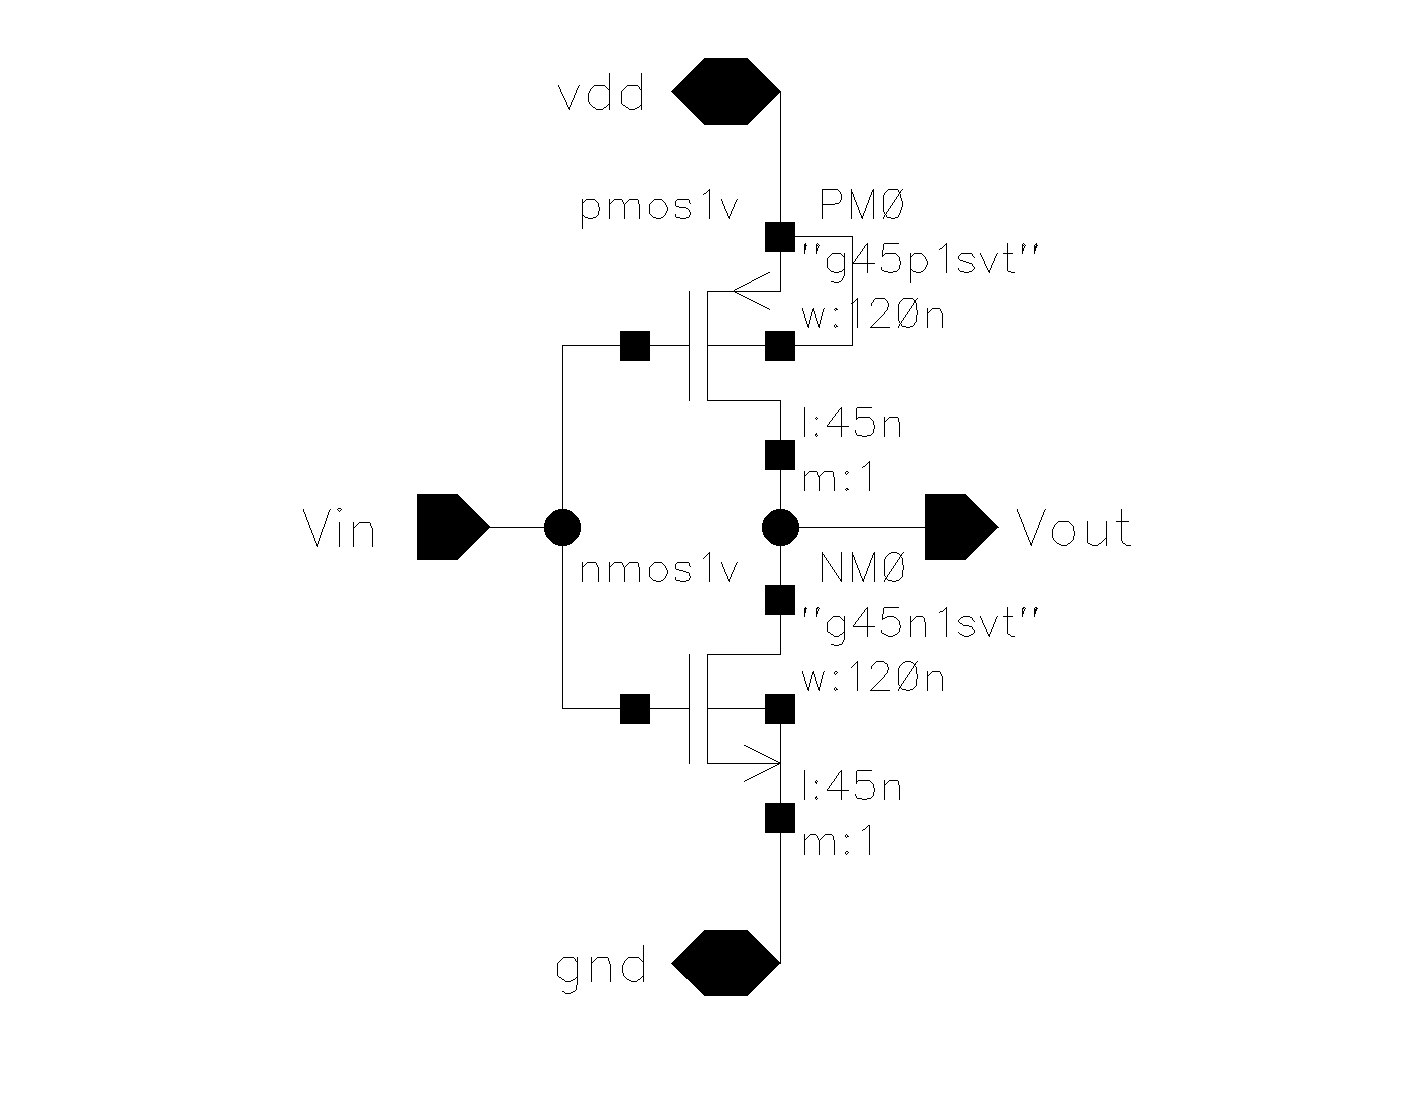
\includegraphics[width=0.5\linewidth]{writeup//figures/inv_sch.png}
    \caption{}
\end{figure}

\subsubsection*{Symbol}

\begin{figure}[H]
    \centering
    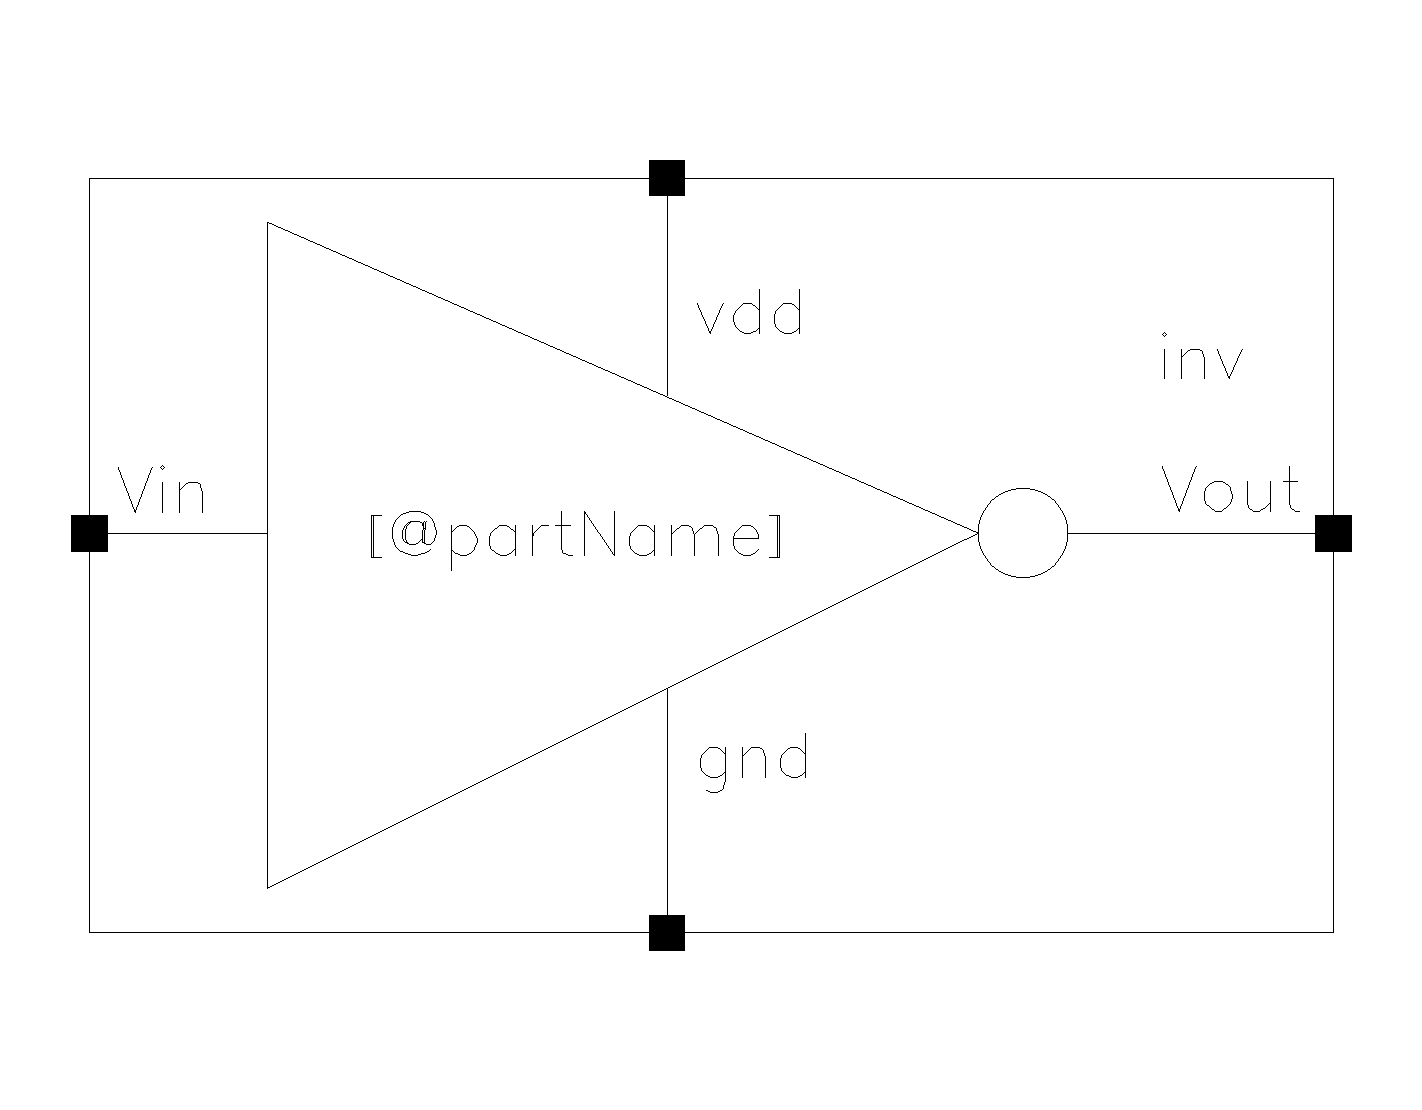
\includegraphics[width=0.5\linewidth]{writeup//figures/inv_sym.png}
    \caption{}
\end{figure}

\newpage

\subsection{2:1 MUX Design}

\subsubsection*{Schematic}

\begin{figure}[H]
    \centering
    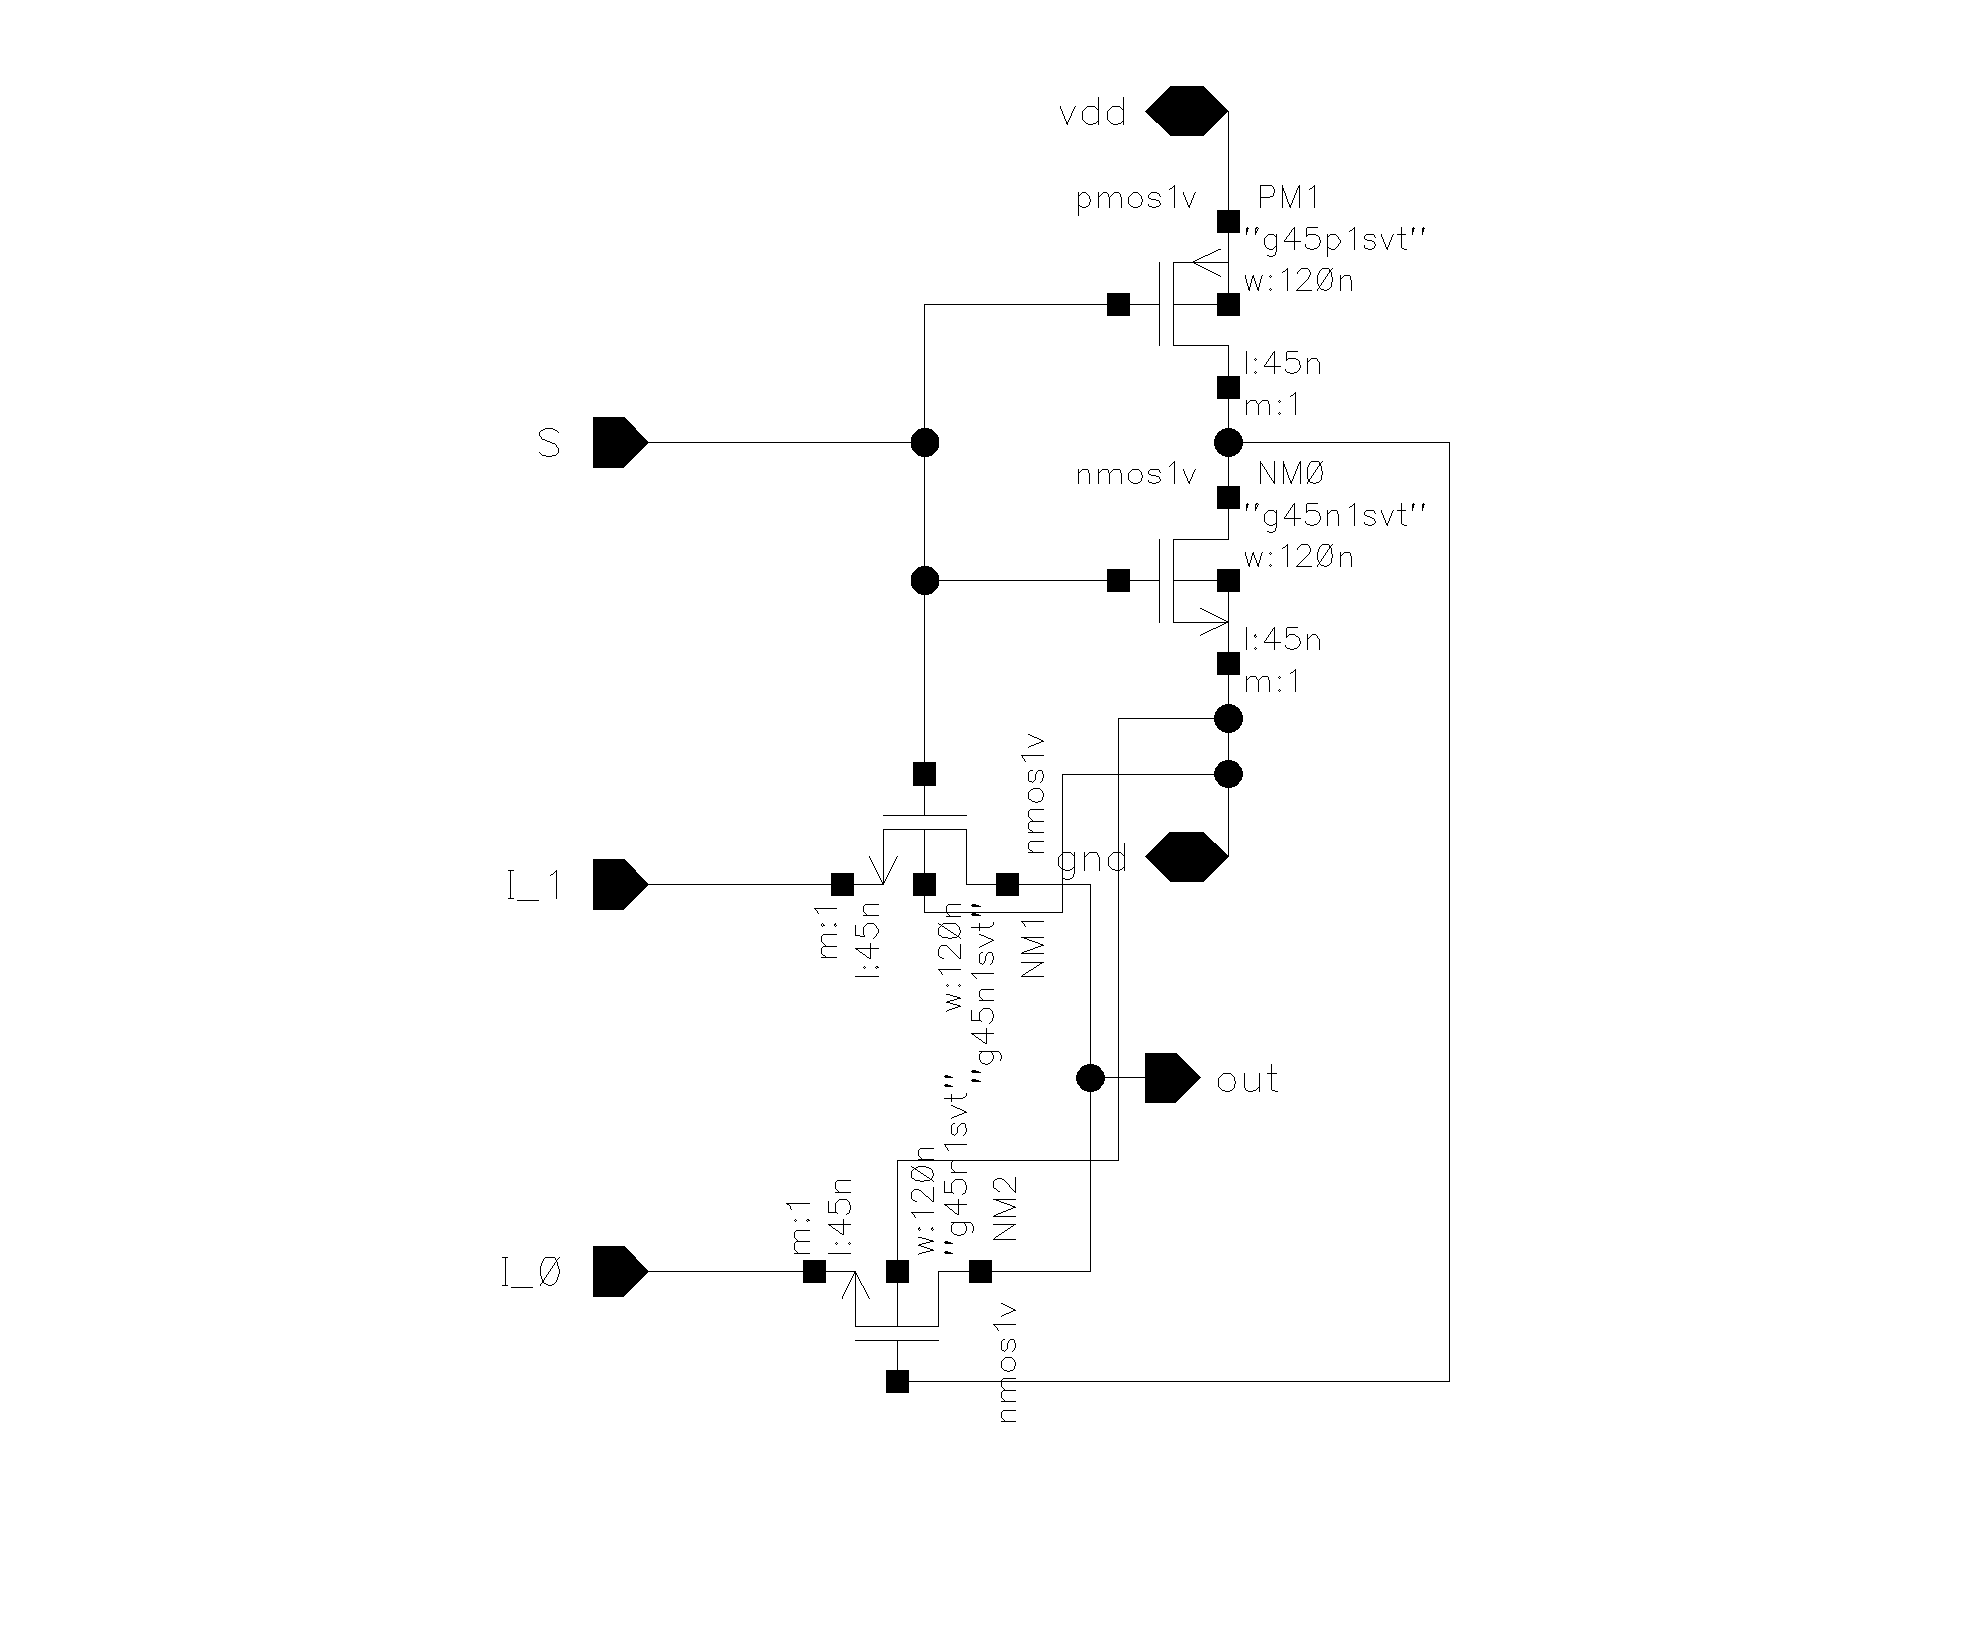
\includegraphics[width=0.8\linewidth]{writeup//figures/MUX_sch.png}
    \caption{}
\end{figure}

\subsubsection*{Symbol}

\begin{figure}[H]
    \centering
    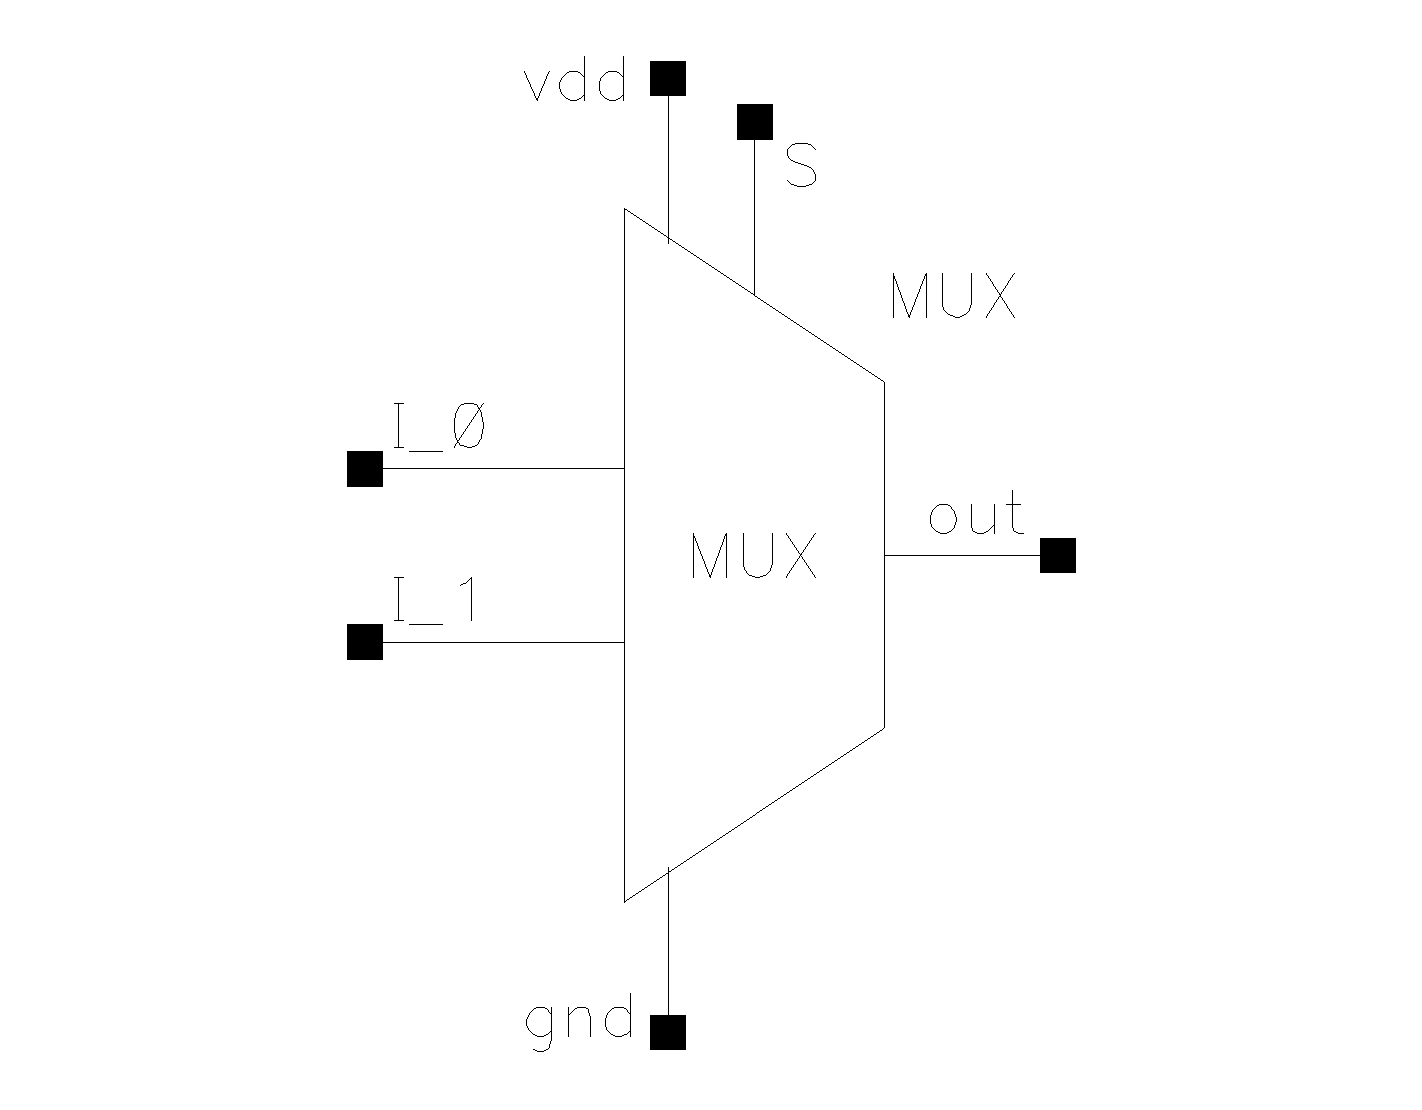
\includegraphics[width=0.5\linewidth]{writeup//figures/MUX_sym.png}
    \caption{}
\end{figure}

\newpage

\subsection{16:1 LUT Design}
\subsubsection*{Schematic}
\begin{figure}[H]
    \centering
    \includegraphics[width=0.5\linewidth]{writeup//figures/LUT_sch.png}
    \caption{}
\end{figure}

\subsubsection*{Symbol}
\begin{figure}[H]
    \centering
    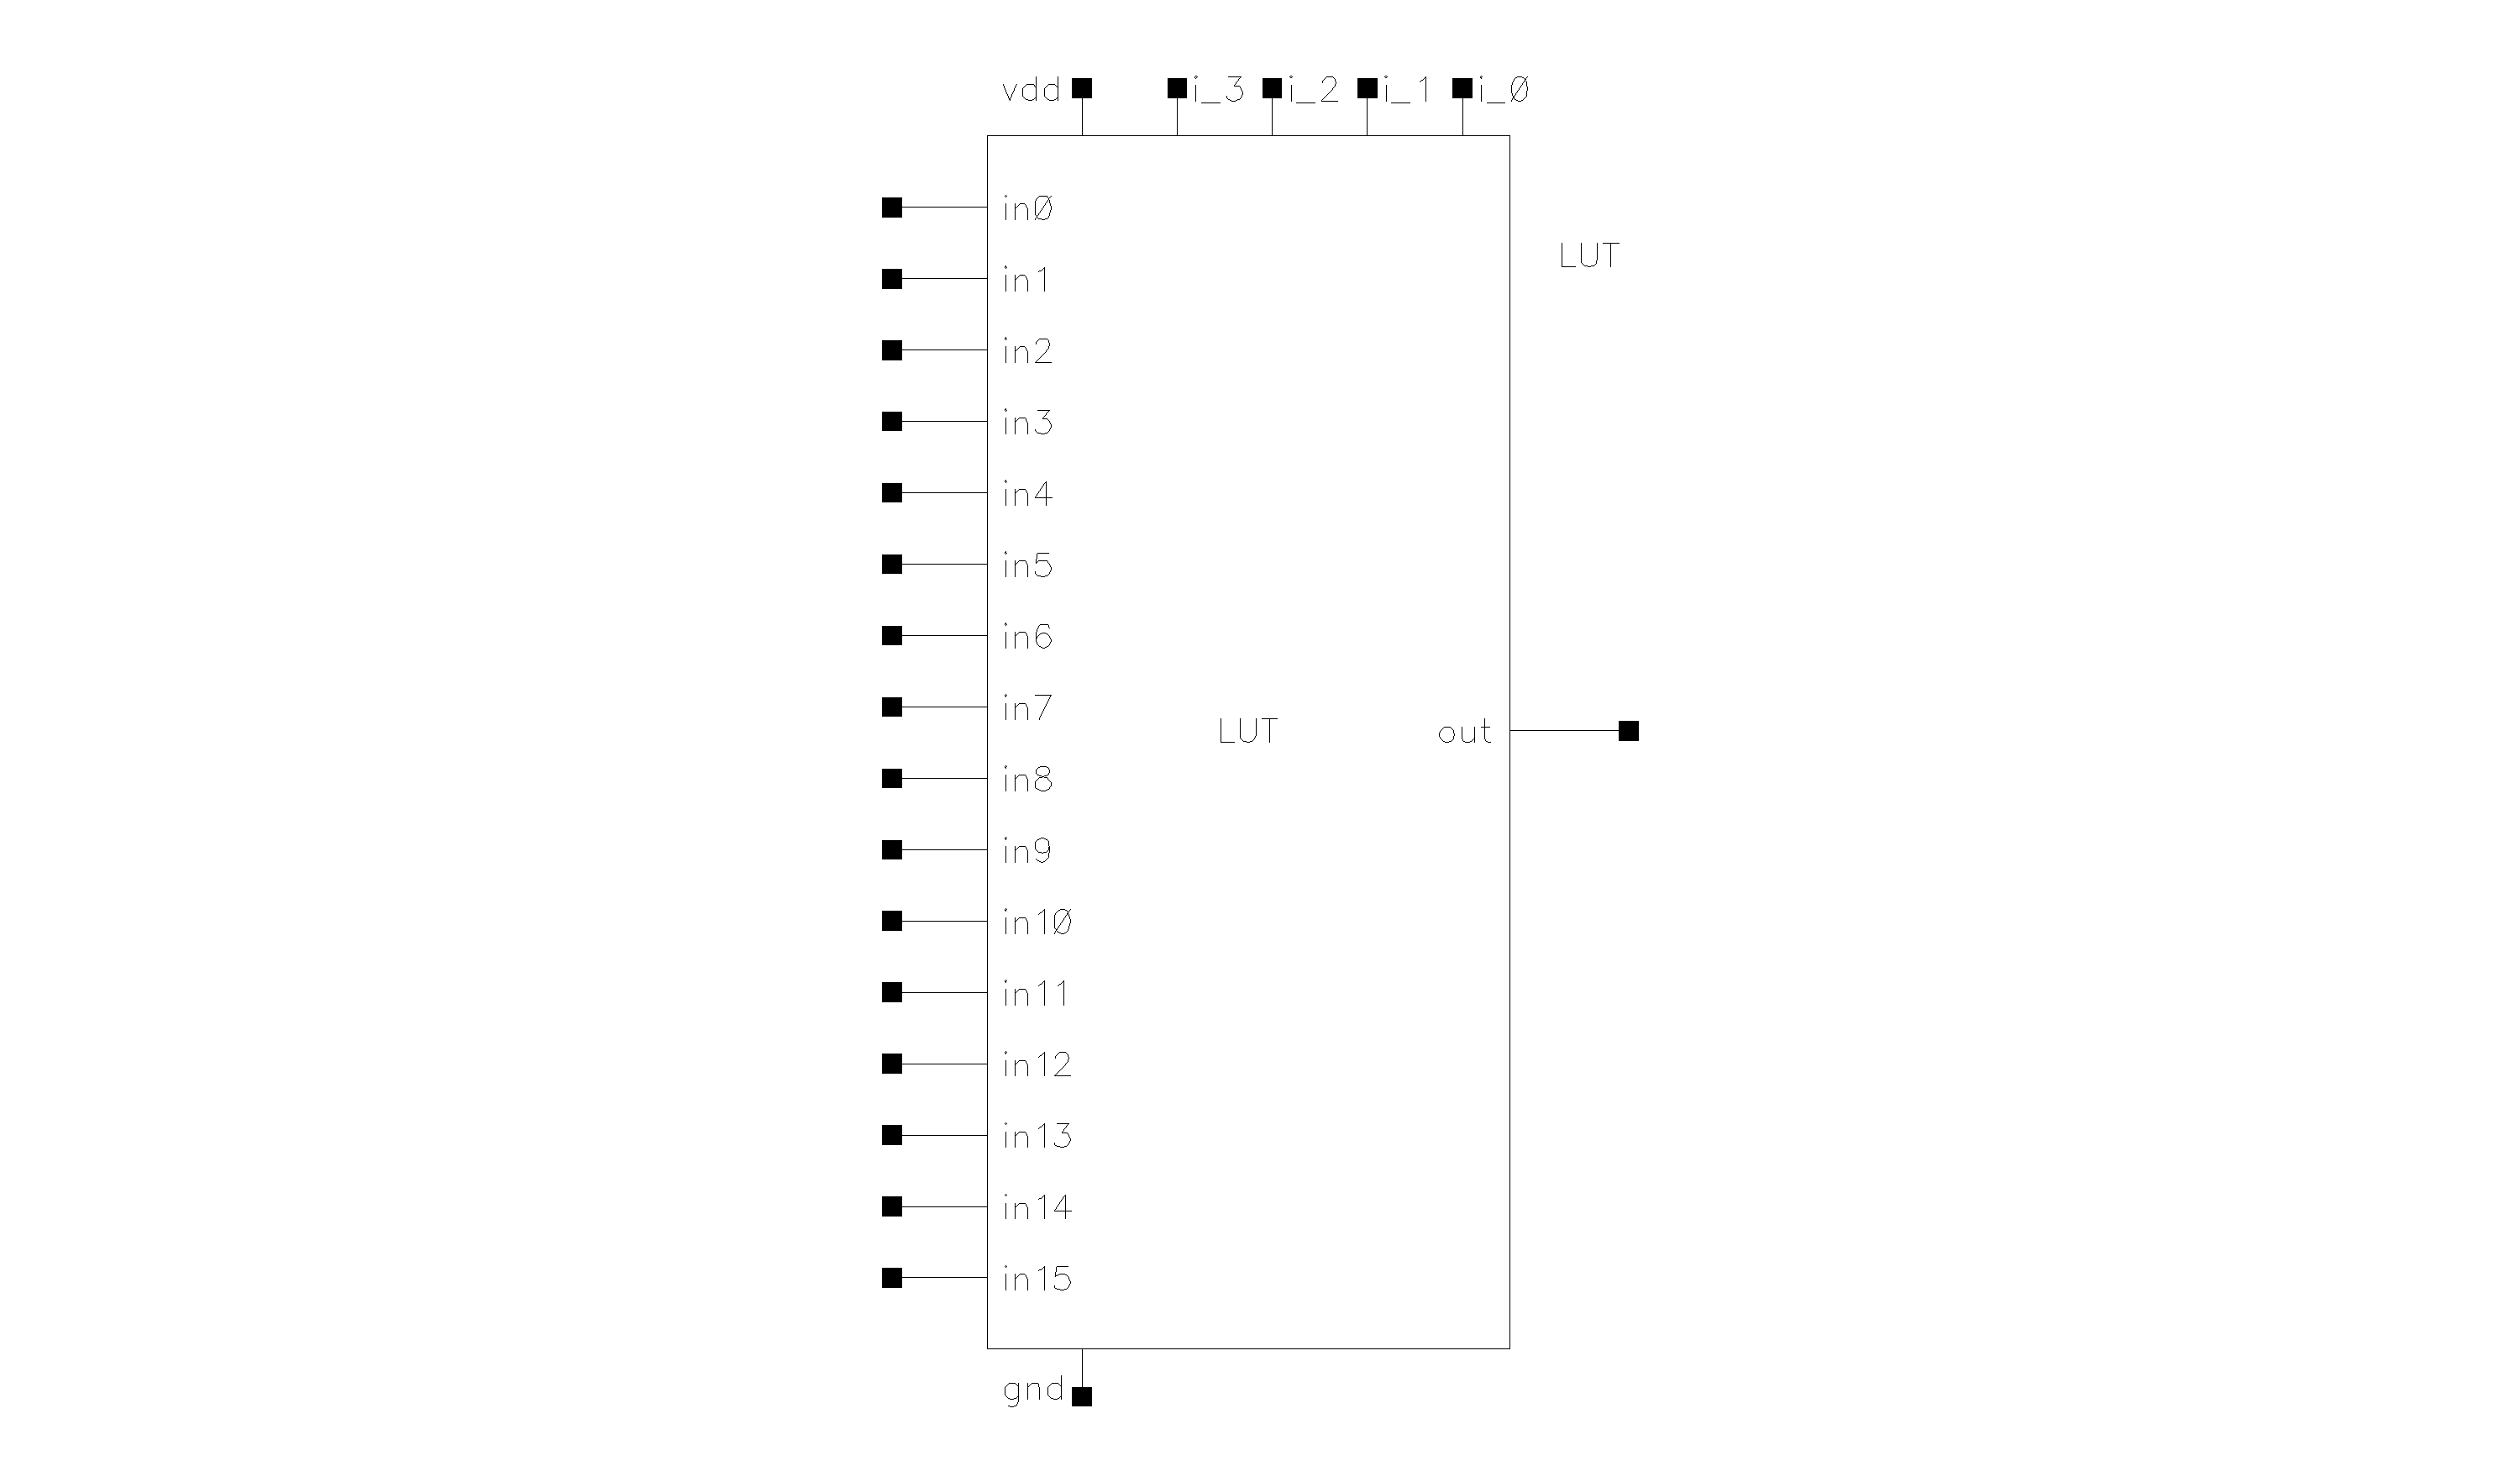
\includegraphics[width=0.8\linewidth]{writeup//figures/LUT_sym.png}
    \caption{}
\end{figure}

\newpage

% ------------------ SECTION 2 ------------------
\section{Baseline Design Validation and Logical Test}
\subsection{Test Schematic and Case}
\subsubsection*{Test Schematics}

\begin{figure}[H]
    \centering
    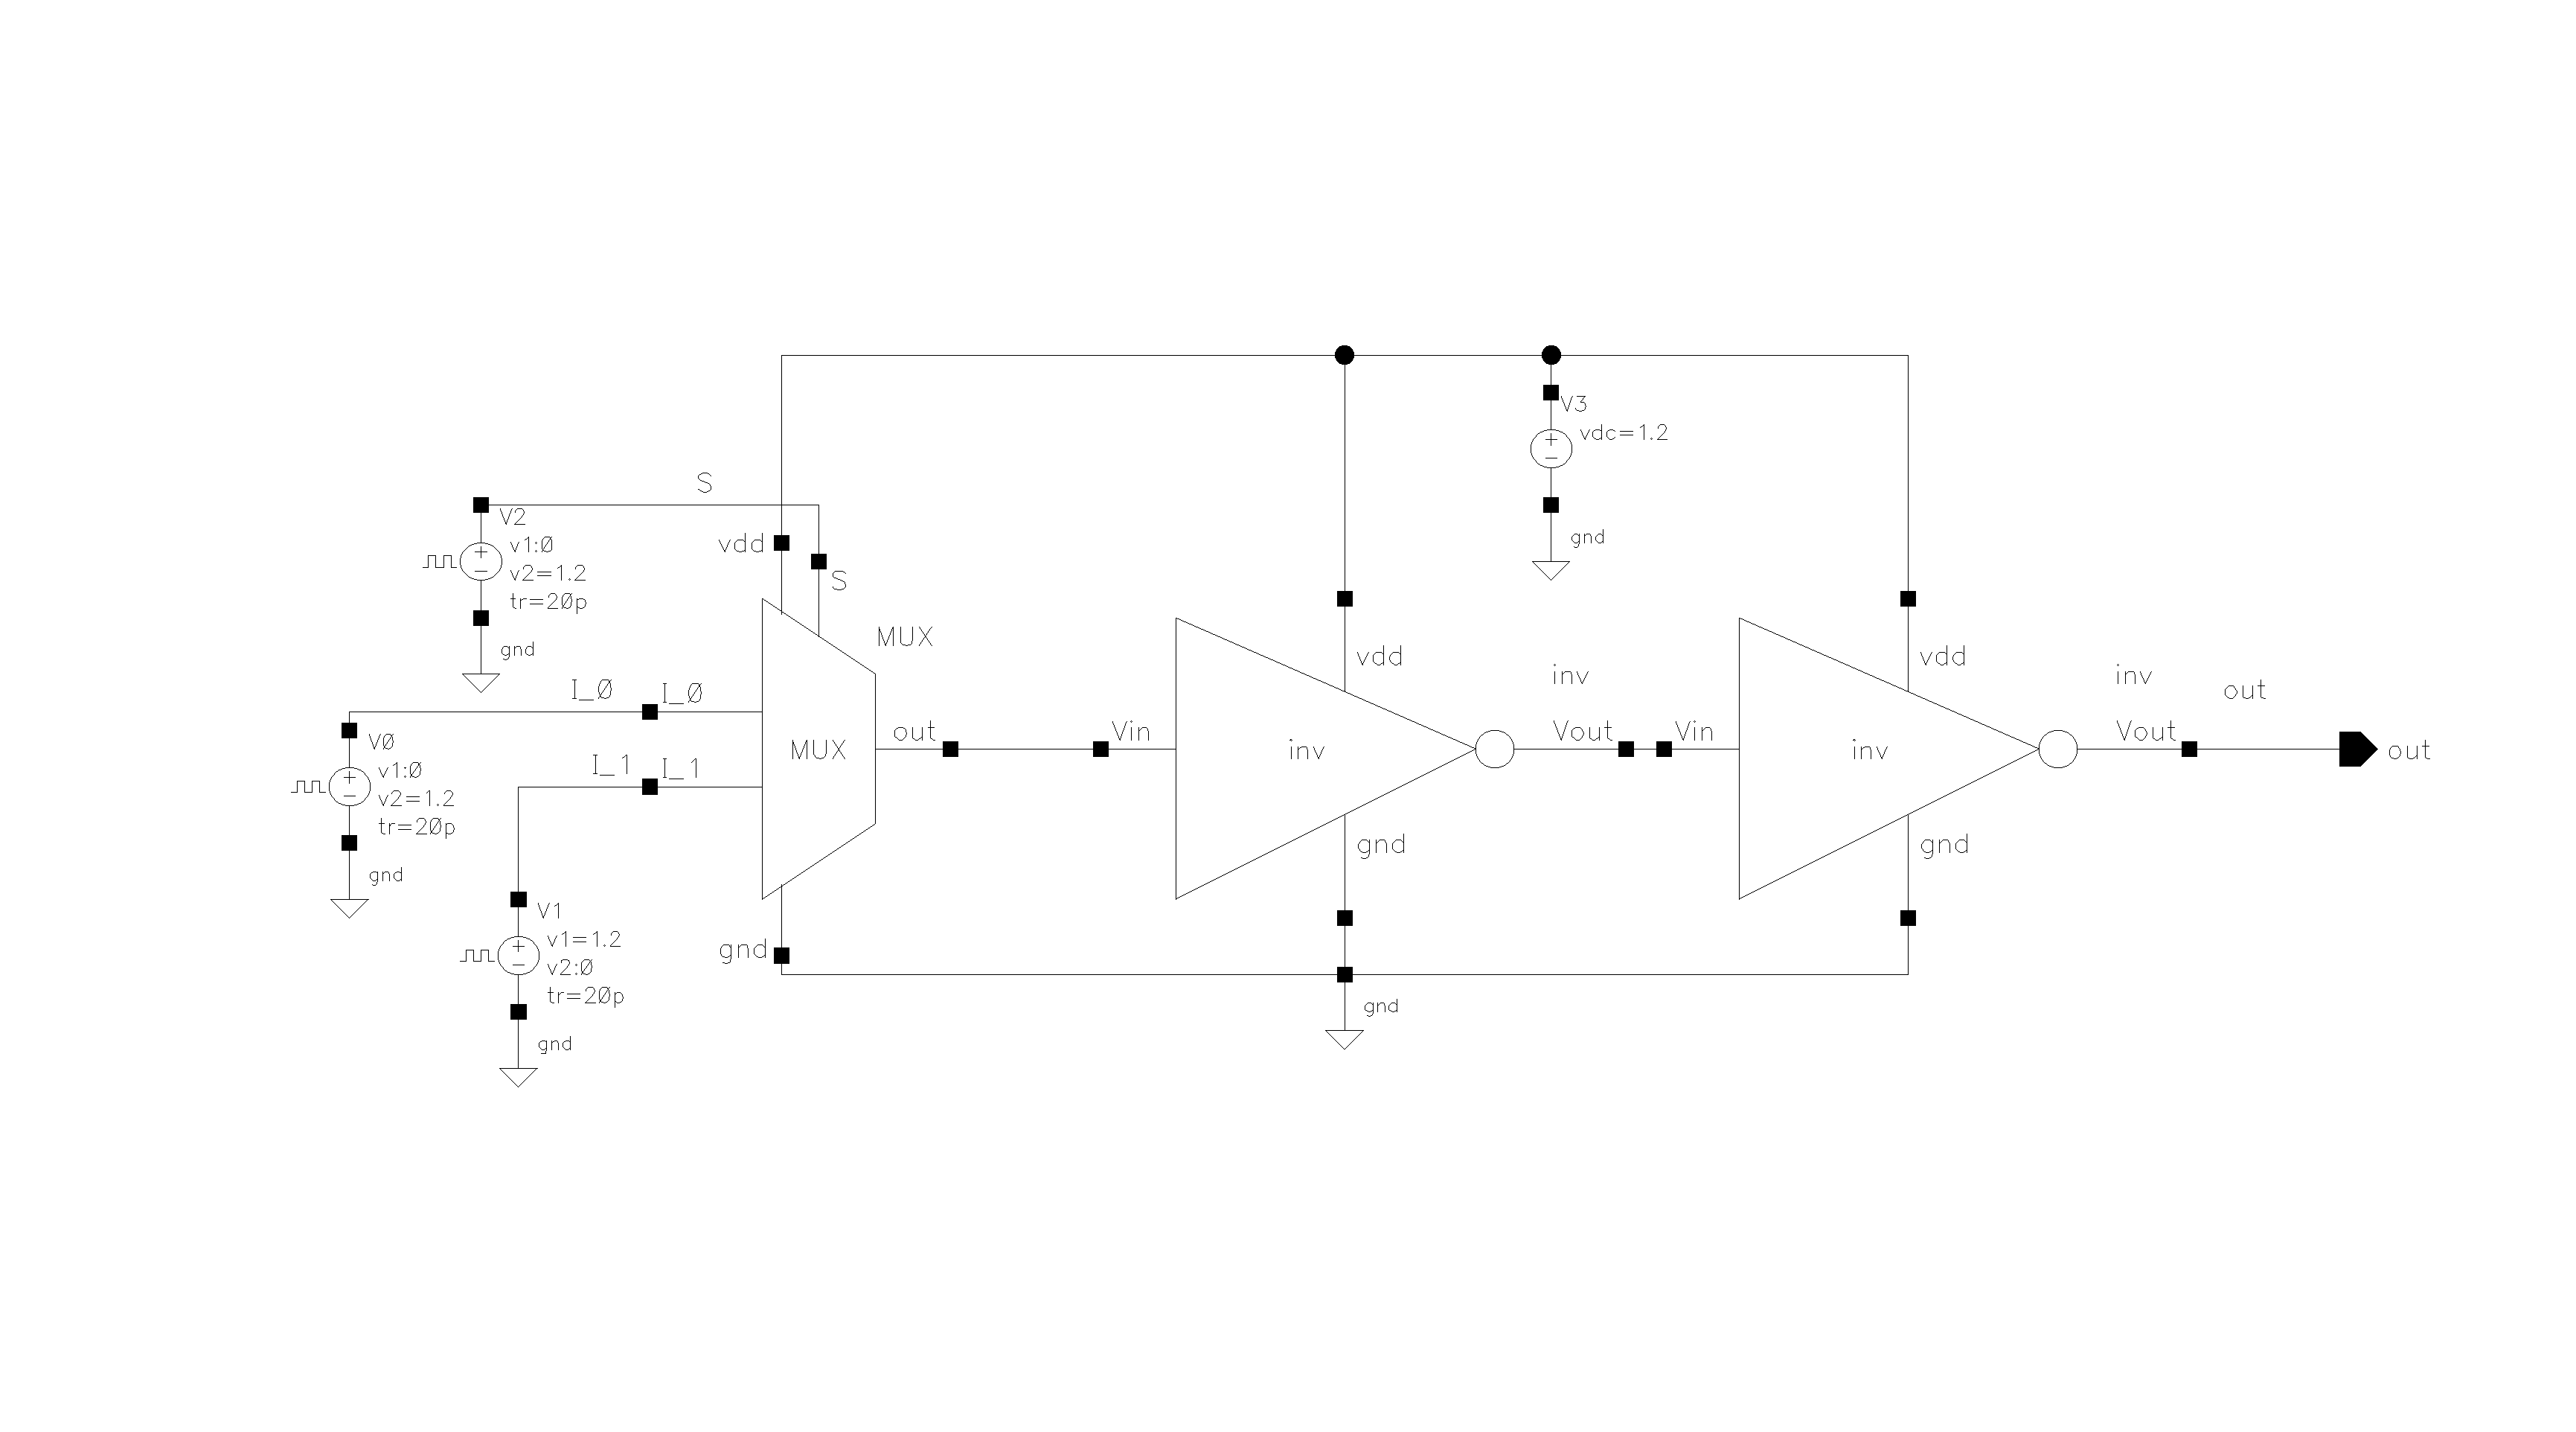
\includegraphics[width=\linewidth]{writeup//figures/muxsubtestschem.png}
    \caption{}
\end{figure}

\begin{figure}[H]
    \centering
    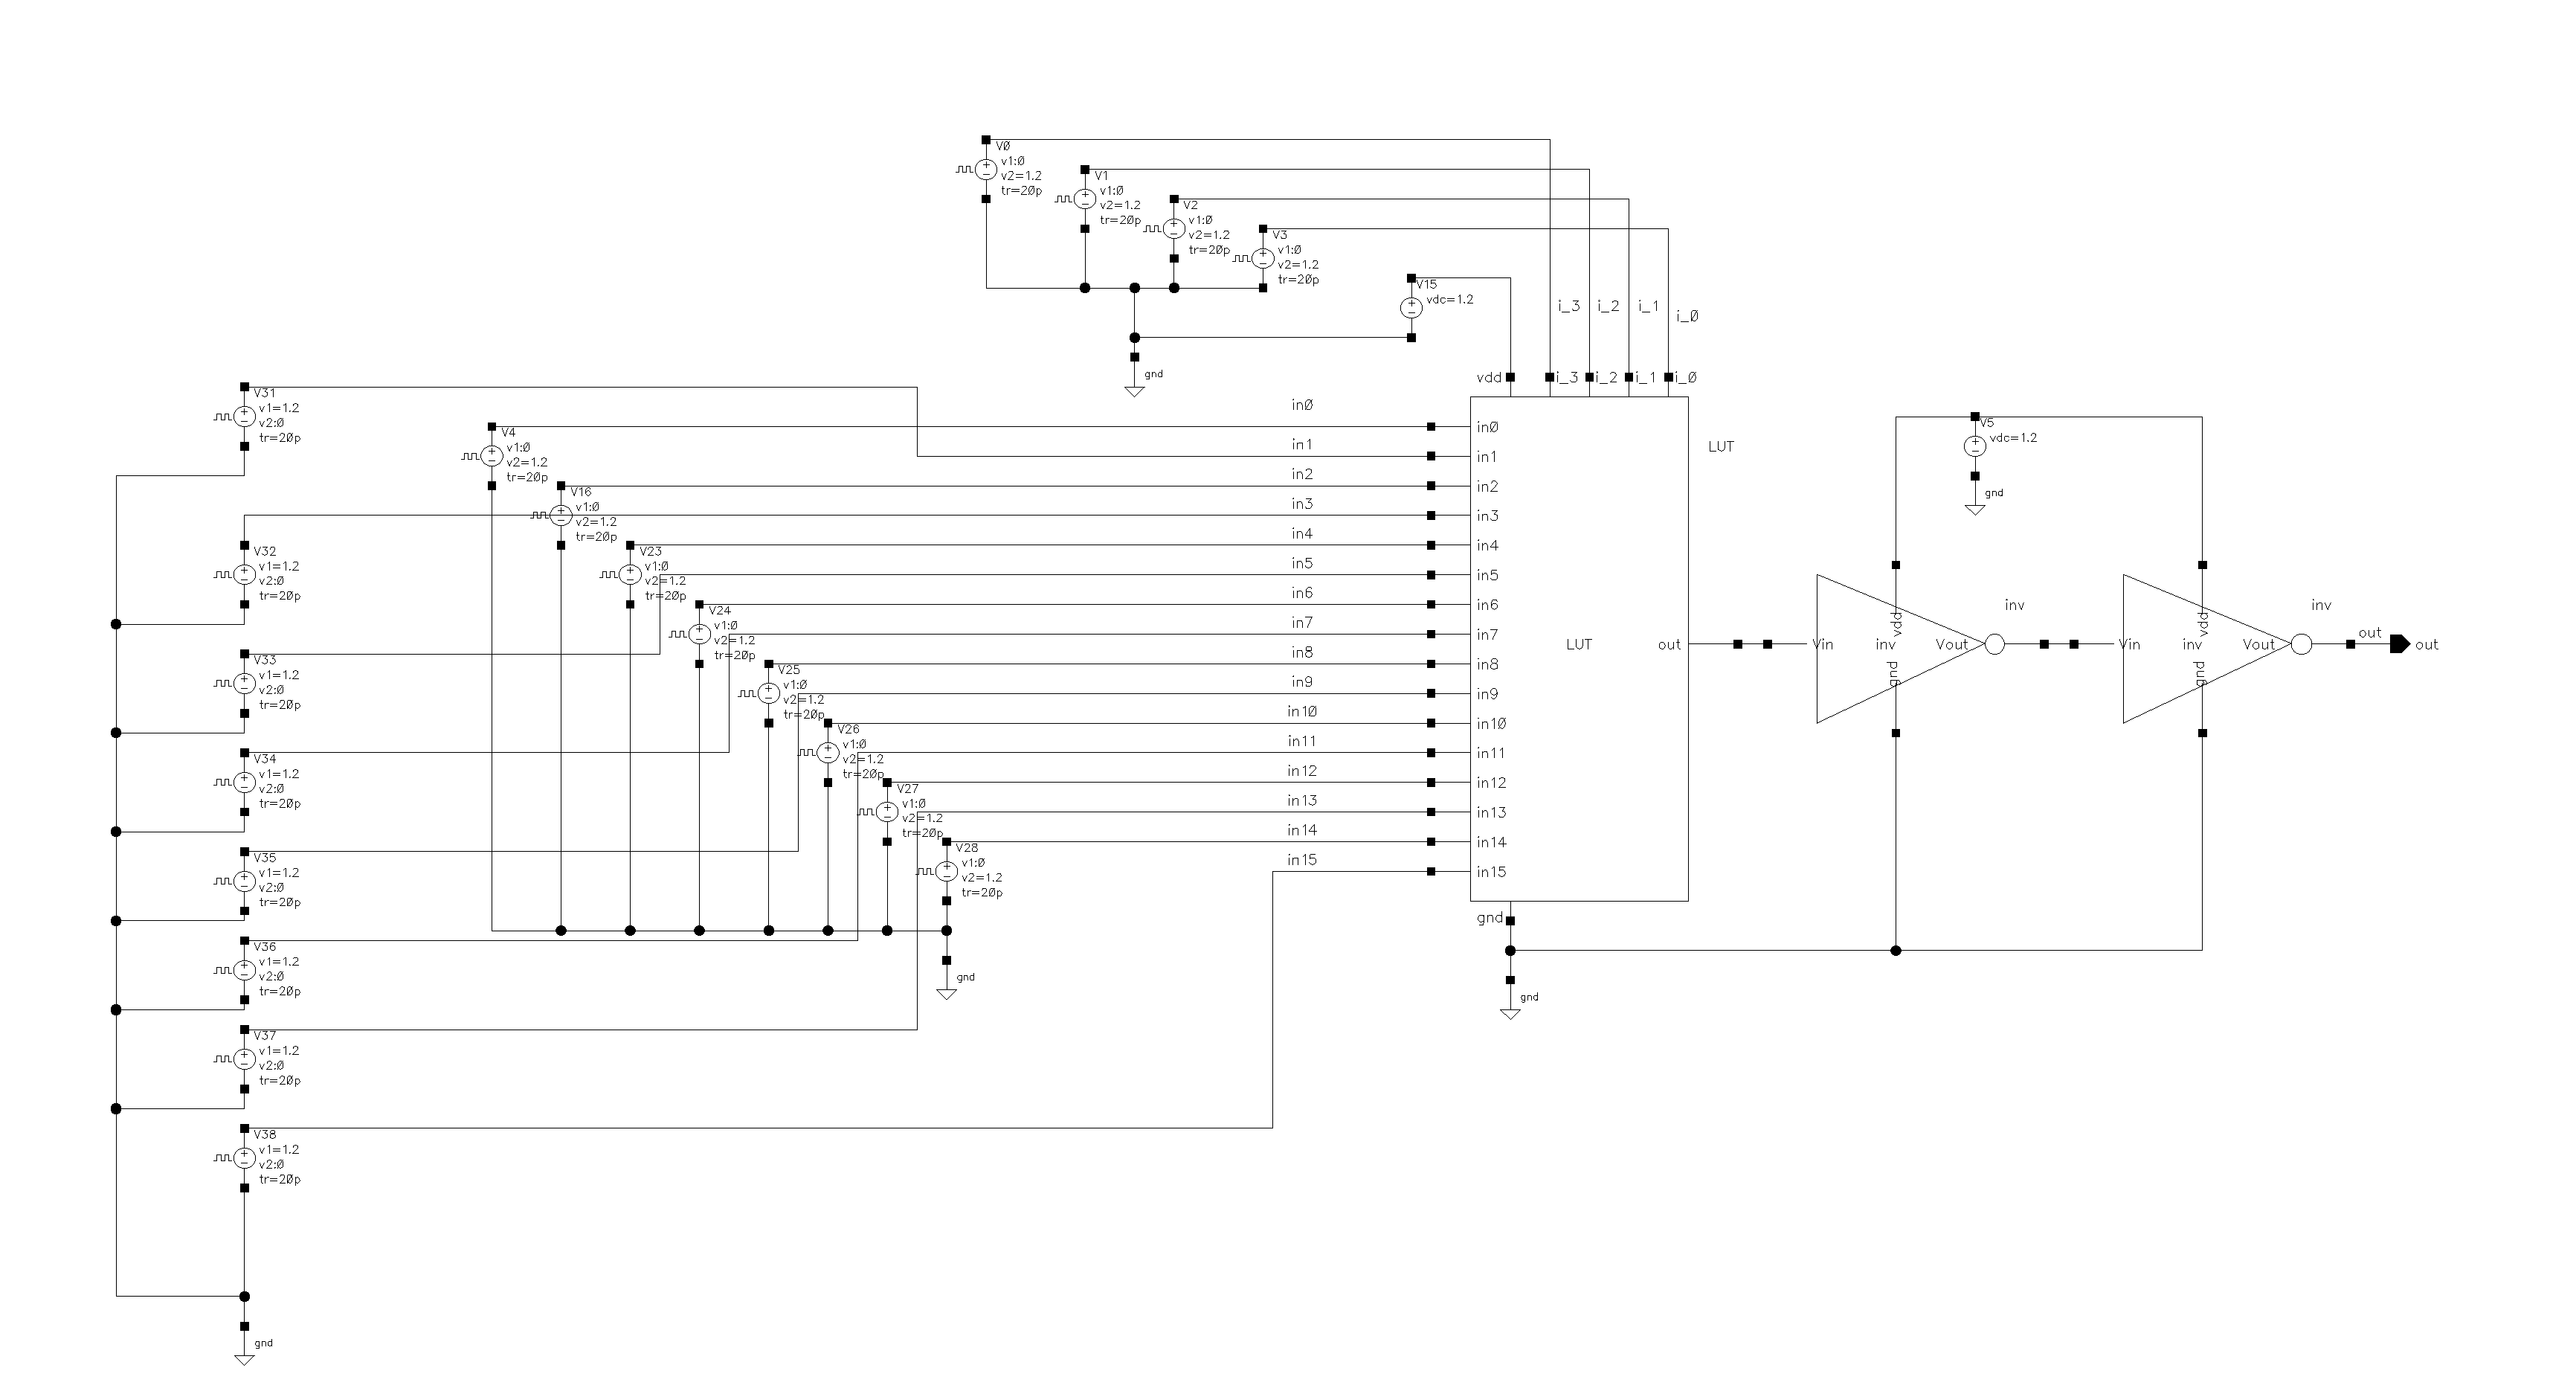
\includegraphics[width=0.8\linewidth]{writeup//figures/luttestschem.png}
    \caption{}
\end{figure}

\subsubsection*{Cases}
For the 2:1 MUX validation, the input signals were configured to ensure that both selection paths could be distinctly verified. The data input \( I_1 \) was driven with a square wave transitioning from low to high, while \( I_0 \) was driven with an inverse square wave (high to low). The select line \( S \) was given a signal with \textbf{double the period} of the data inputs to allow for multiple transitions of \( I_0 \) and \( I_1 \) within each select cycle. 
This setup ensures that during each half-period of \( S \), both data inputs experience a full logic transition, allowing the output to alternate between following \( I_0 \) and \( I_1 \) depending on the state of \( S \). 
By measuring the output \( V_{\text{out}} \) and observing that it follows \( I_1 \) when \( S=1 \) and \( I_0 \) when \( S=0 \), the expected multiplexer behavior was confirmed. The corresponding transient waveform verified this switching behavior with minimal propagation delay between the input and output transitions.

For the 16:1 LUT validation, a counter-type input pattern was applied to systematically generate all \( 2^4 = 16 \) address combinations. 
Each address line was assigned a different pulse period to form a binary counting sequence: \( I_3 \) with a 2\,ns period, \( I_2 \) with 4\,ns, \( I_1 \) with 8\,ns, and \( I_0 \) with 16\,ns. This timing scheme ensures that over one full 16-state cycle, every unique combination from \( 0000 \) to \( 1111 \) is applied to the address inputs. All sixteen data inputs (\( \text{IN}_0 \) through \( \text{IN}_{15} \)) were driven with identical 8\,ns square waves to maintain consistent signal activity. 
As the address counter advanced, the output \( V_{\text{out}} \) was observed to follow the corresponding data input for each address state, verifying correct selection logic and full LUT functionality.

\newpage

\subsection{Validation}
\subsubsection*{2:1 MUX Subcircuit Validation}
\begin{figure}[H]
    \centering
    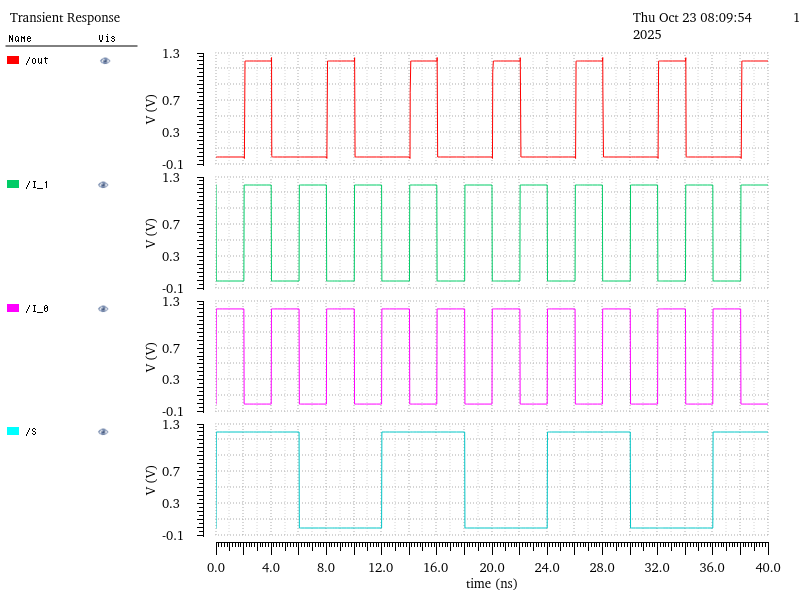
\includegraphics[width=\linewidth]{writeup//figures/muxsubval.png}
    \caption{}
\end{figure}

In the subcircuit test, the select input \( S \) is toggled while \( I_0 \) and \( I_1 \) run as independent square waves. 
Whenever \( S \) is high, the output waveform overlays \( I_1 \) with only a small propagation delay; whenever \( S \) is low, the output overlays \( I_0 \). 
Each handoff can be observed at the transitions of \( S \): during every \( S=1 \) interval the output \( V_{\text{out}} \) matches \( I_1 \), and during every \( S=0 \) interval it matches \( I_0 \). 
This behavior corresponds to the expected logic equation 
\[
V_{\text{out}} = S \cdot I_1 + \overline{S} \cdot I_0
\]
for a 2:1 pass-gate multiplexer. 
The simulation therefore verifies that the subcircuit operates correctly.

\newpage

\subsubsection*{16:1 LUT Validation}
\begin{figure}[H]
    \centering
    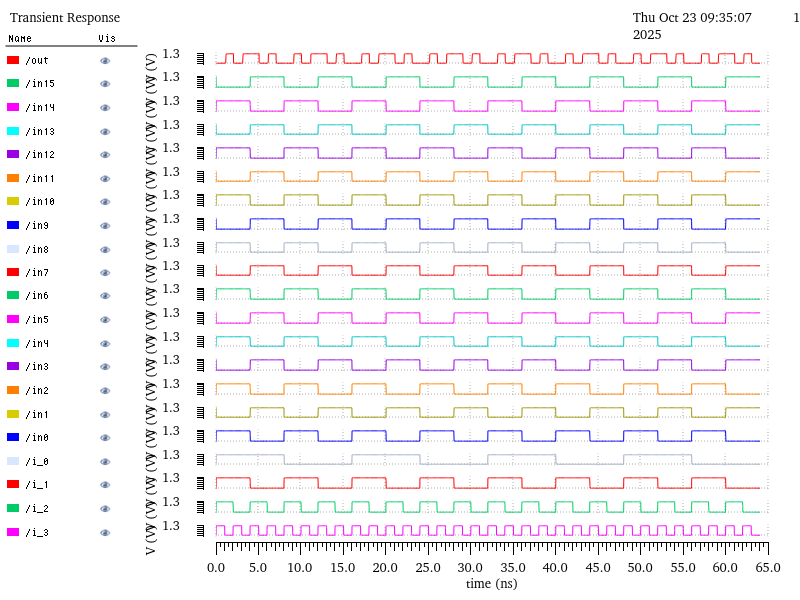
\includegraphics[width=\linewidth]{writeup//figures/lutval.png}
    \caption{}
\end{figure}

For the full 16:1 LUT, all sixteen input combinations (\(2^4\)) were simulated by varying the four address lines from \(0000\) through \(1111\). 
In each address state, the output \(V_{\text{out}}\) aligns with exactly one corresponding data input. 
Specifically, when the address equals \(0000\), \(\text{IN}_0\) propagates to the output; as the address increments, \(\text{IN}_1, \text{IN}_2, \ldots, \text{IN}_{15}\) sequentially drive the output. 
Rising and falling edges on \(V_{\text{out}}\) coincide precisely with the selected input, while nonselected inputs show no coupling. 
Because all address combinations were verified and the output correctly reflected the selected data input each time, the 16:1 LUT simulation confirms correct functionality.

\newpage

% ------------------ SECTION 3 ------------------
\section{Baseline Delay Measurement}
\subsection{Test Schematic}

\begin{figure}[H]
    \centering
    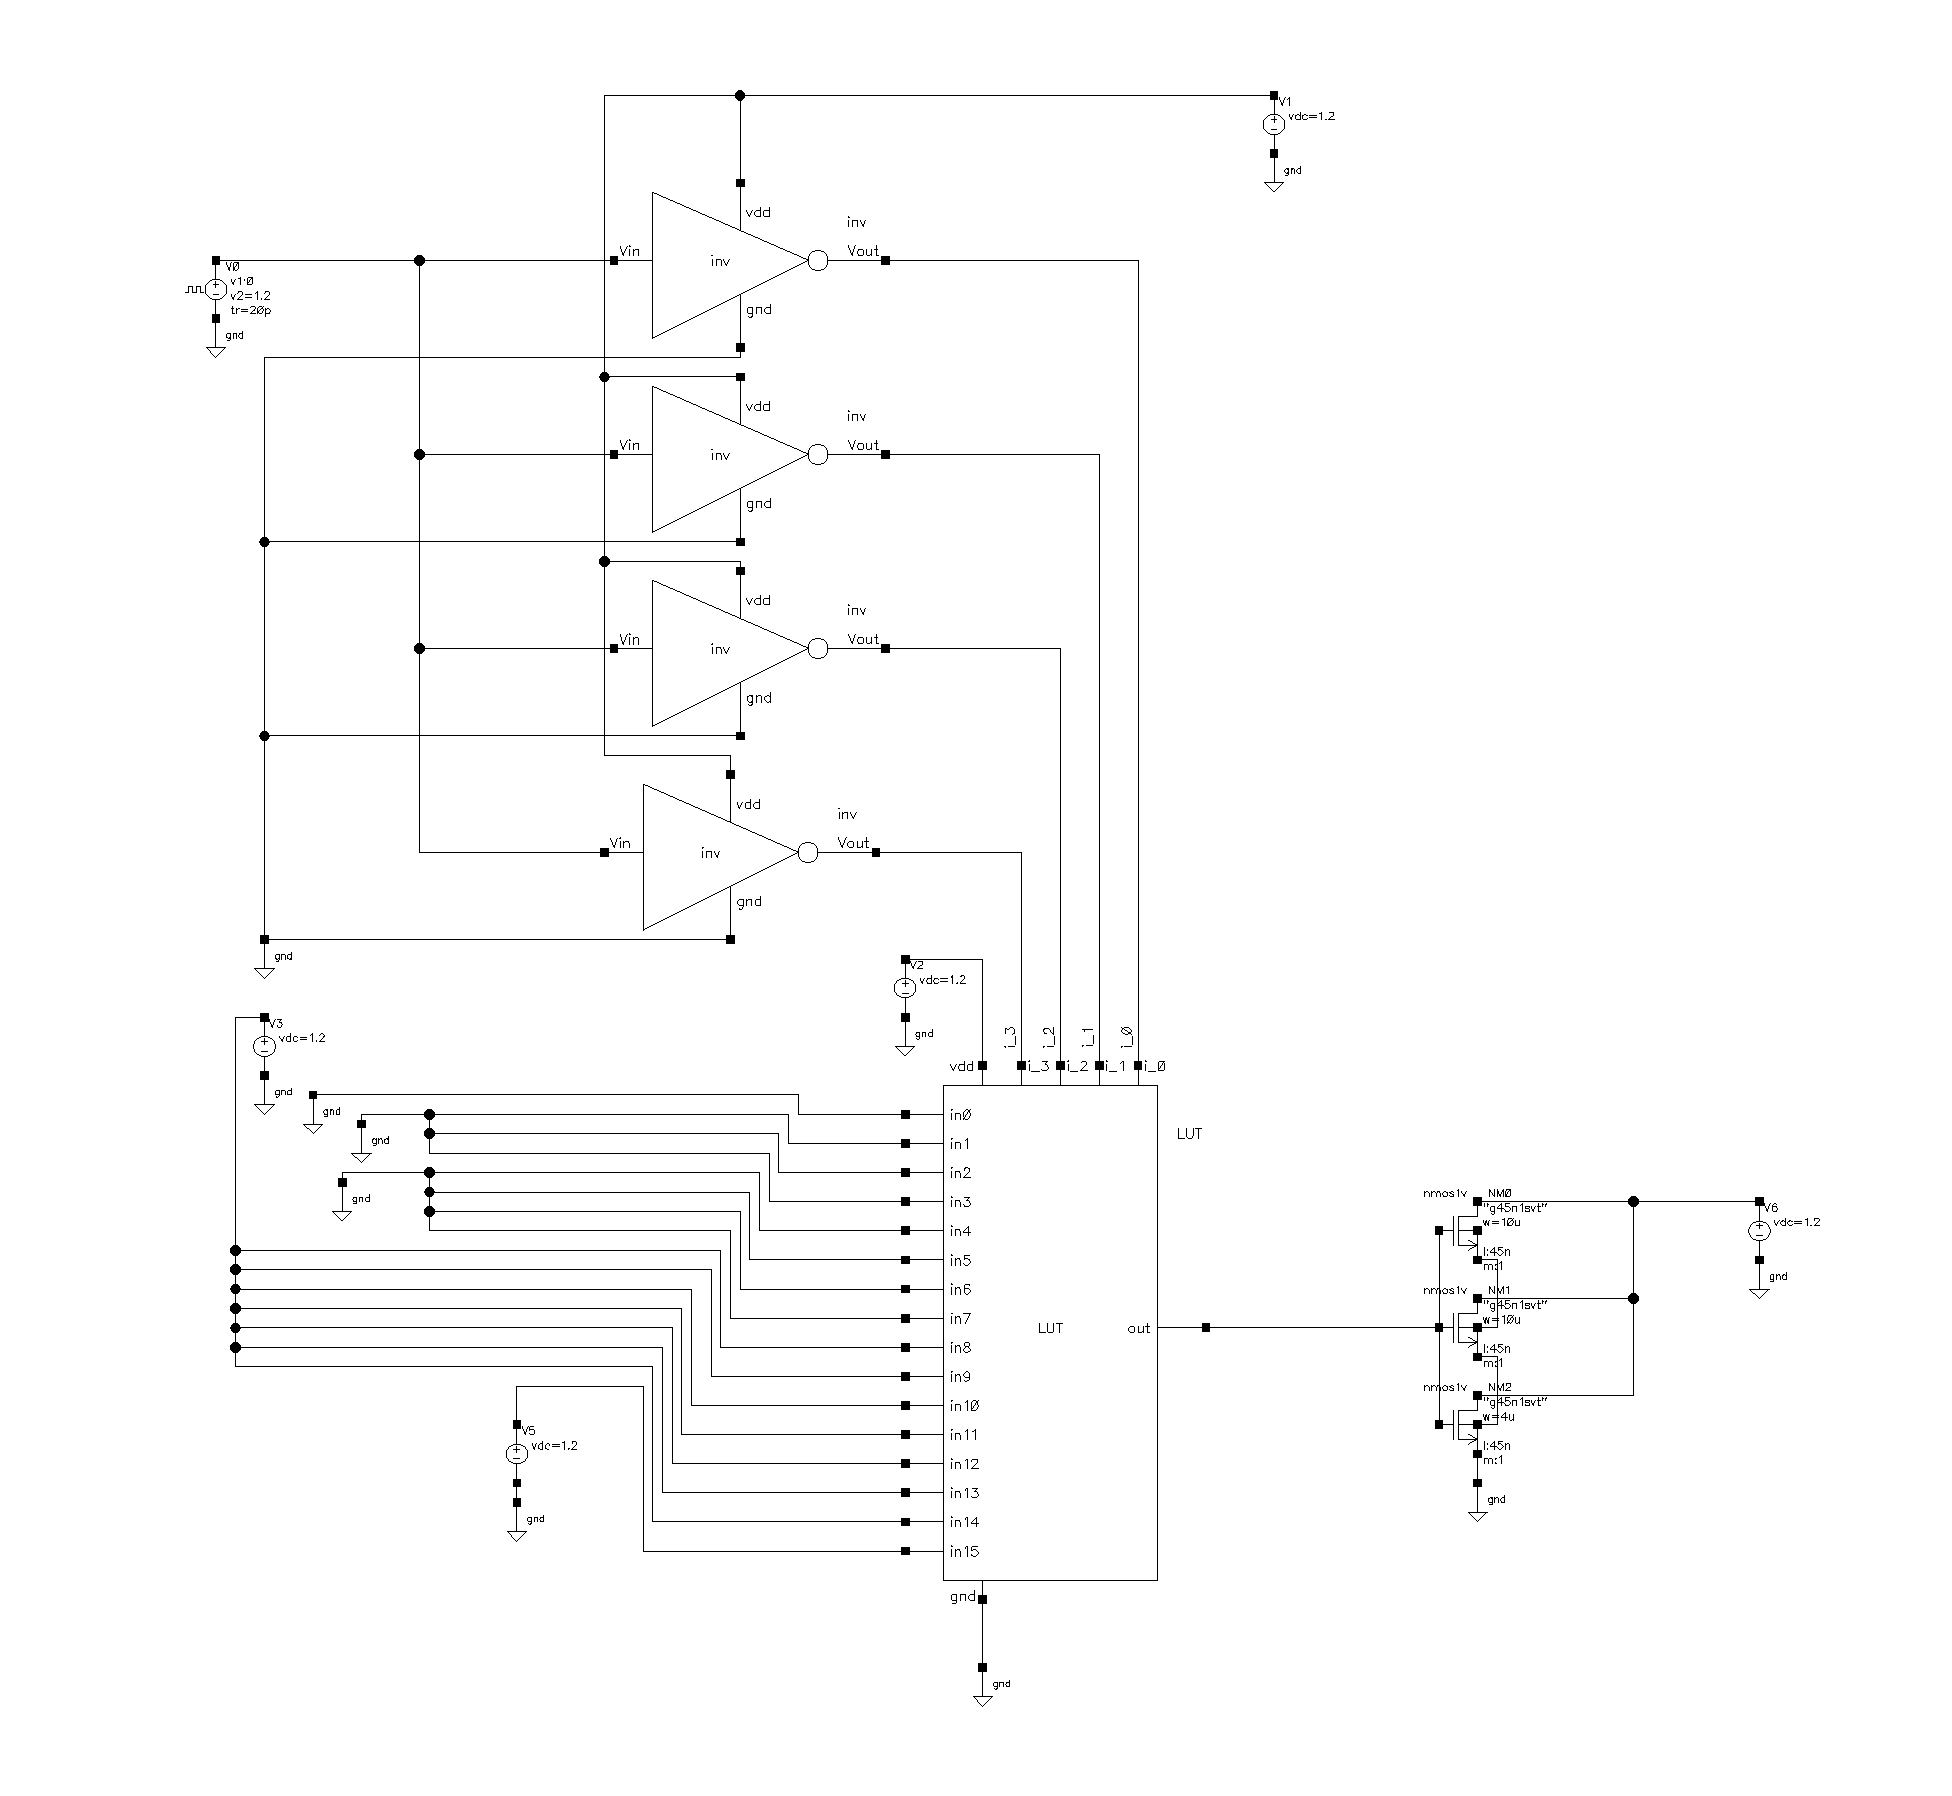
\includegraphics[width=\linewidth]{writeup//figures/lut_delay_testbench.png}
    \caption{}
\end{figure}

\newpage

\subsection{Test Case}
To evaluate the worst-case propagation delay of the 16:1 LUT, the input configuration was chosen to isolate the longest signal path through the multiplexer tree. 
Data inputs \(\text{IN}_0\) through \(\text{IN}_7\) were tied to ground (\(0\,\text{V}\)), while \(\text{IN}_8\) through \(\text{IN}_{15}\) were connected to \(V_{DD}\). 
Separate ground and \(V_{DD}\) connections were provided for \(\text{IN}_0\) and \(\text{IN}_{15}\), since these represent the boundary input cases that the output \(V_{\text{out}}\) would follow depending on the address configuration under test. 

The four address lines (\(I_0, I_1, I_2, I_3\)) were driven by \texttt{Vpulse} sources transitioning from low to high, generating the binary address sequence from \(0000\) to \(1111\). 
Switching all address inputs from 0 to 1 allowed the LUT to traverse every possible address combination, ensuring that the output response was tested across the full range of input states. 
This transition sequence also activates the critical switching path, as multiple internal MUX stages change simultaneously, causing maximum internal toggling and delay. 
Because \(I_3\) acted as the least significant bit (LSB), the signal path corresponding to \(I_3\) produced the longest propagation path through the multiplexer hierarchy and thus determined the worst-case delay.

At the output node, three NMOS transistors with widths of \(10\,\mu\text{m}\), \(10\,\mu\text{m}\), and \(4\,\mu\text{m}\) were connected in parallel to form an equivalent capacitive loading of approximately \(200C_g\). 
Given the minimum device width of \(120\,\text{nm}\), a total effective width of \(24\,\mu\text{m}\) was required to achieve this load. 
This output loading condition ensured realistic delay measurement under high fan-out, enabling accurate evaluation of the LUT’s timing performance in its worst-case switching scenario.

\newpage

\subsection{Simulation Results and Metric Value}
\begin{figure}[H]
    \centering
    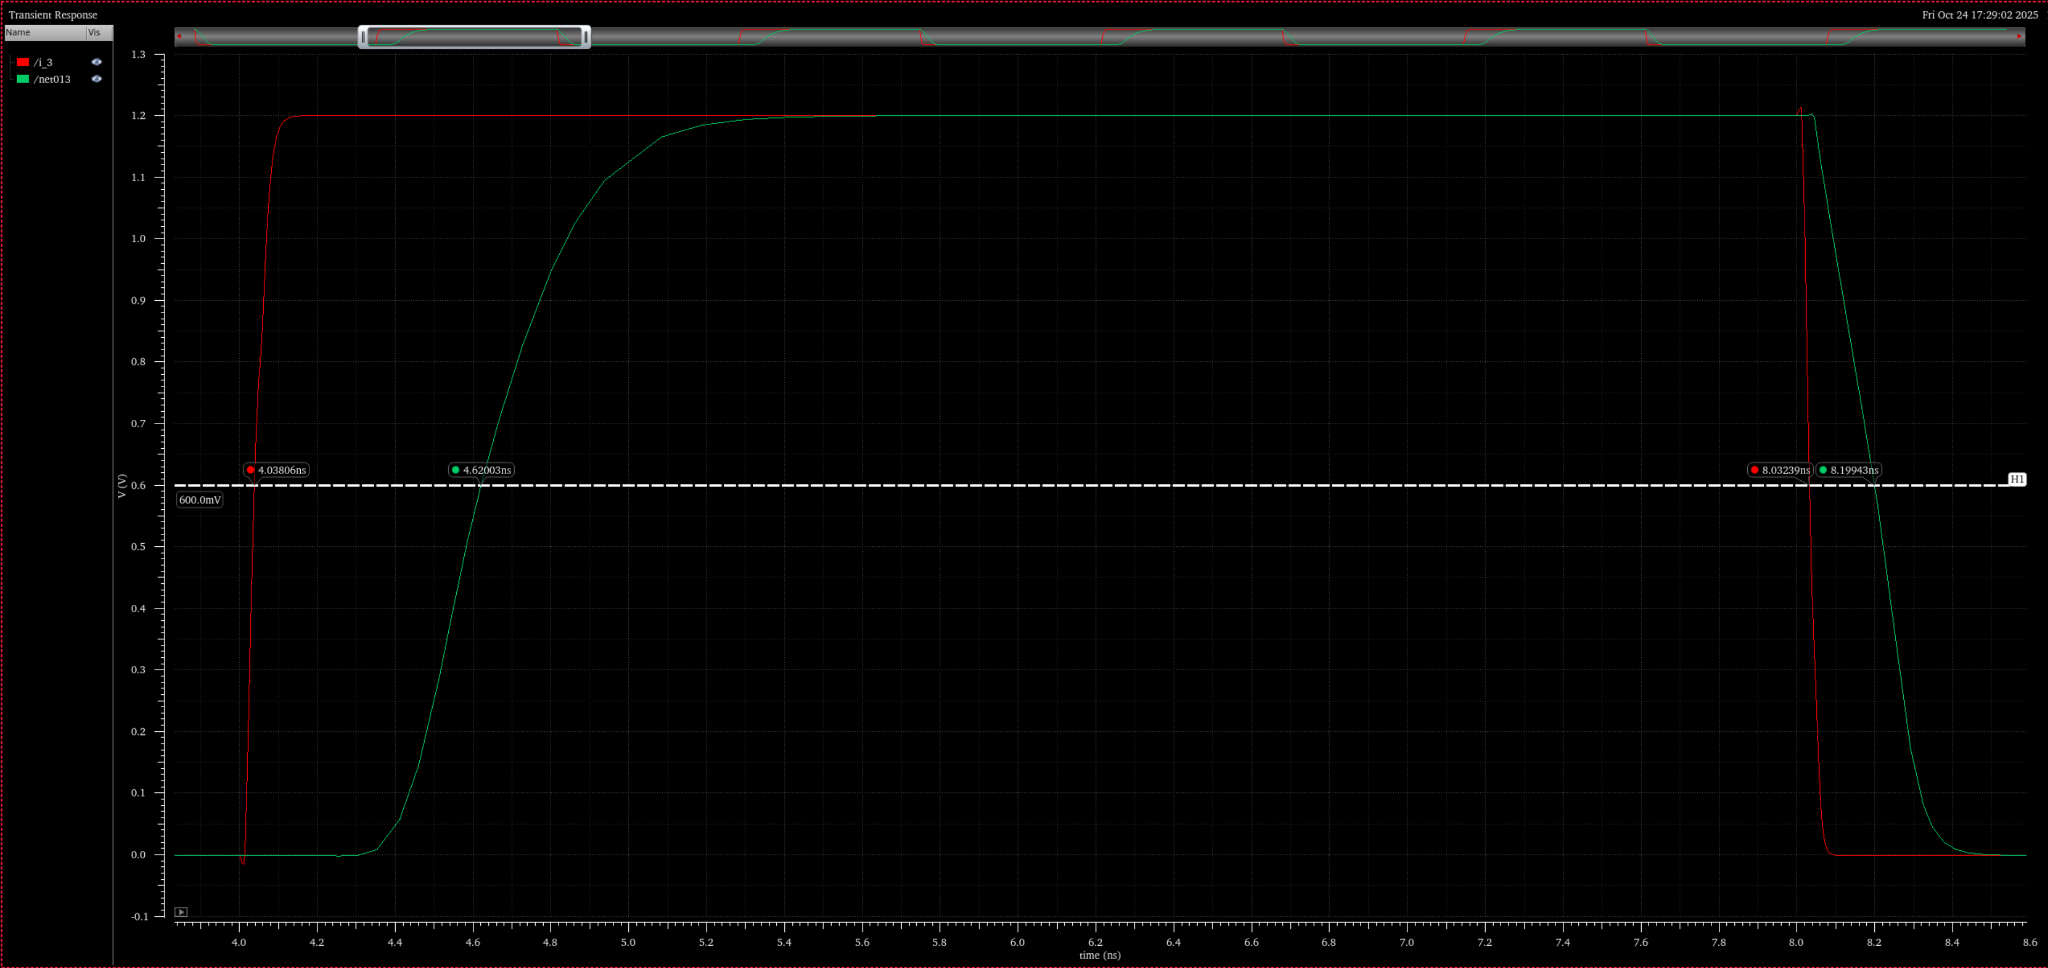
\includegraphics[width=\linewidth]{writeup//figures/baselinedelay.png}
    \caption{}
\end{figure}
Propagation delay measurements are made at the 50\% voltage level of both the input and output signals, which corresponds to \( V = 0.5V_{DD} = 0.6\,\text{V} \) for a 1.2\,V supply.

\subsubsection*{Low-to-High Transition (\(t_{PLH}\))}

For the rising output transition:
\[
t_{PLH} = t_{\text{out,50\%↑}} - t_{\text{in,50\%↓}}
\]
Substituting measured values from the transient response:
\[
t_{PLH} = 4.62003\,\text{ns} - 4.03806\,\text{ns} = 0.58197\,\text{ns}
\]

\subsubsection*{High-to-Low Transition (\(t_{PHL}\))}

For the falling output transition:
\[
t_{PHL} = t_{\text{out,50\%↓}} - t_{\text{in,50\%↑}}
\]
\[
t_{PHL} = 8.19943\,\text{ns} - 8.03239\,\text{ns} = 0.16704\,\text{ns}
\]

\subsubsection*{Average and Worst-Case Delay}

The average propagation delay is given by:
\[
t_p = \frac{t_{PLH} + t_{PHL}}{2}
\]
\[
t_p = \frac{0.58197 + 0.16704}{2} = 0.3745\,\text{ns}
\]

The worst-case delay is the longer of the two:
\[
t_{pd,worst} = \max(t_{PLH}, t_{PHL}) = 0.58197\,\text{ns}
\]

From the results, the rising transition (\(t_{PLH}\)) dominates, indicating that the PMOS network contributes more delay due to its higher effective resistance compared to the NMOS pull-down path. 
Therefore, the \textbf{worst-case propagation delay} of the circuit is approximately \(\mathbf{0.582\,ns}\).


\newpage

% ------------------ SECTION 4 ------------------
\section{Baseline Frequency Measurement}
\subsection{Test Schematic}

\begin{figure}[H]
    \centering
    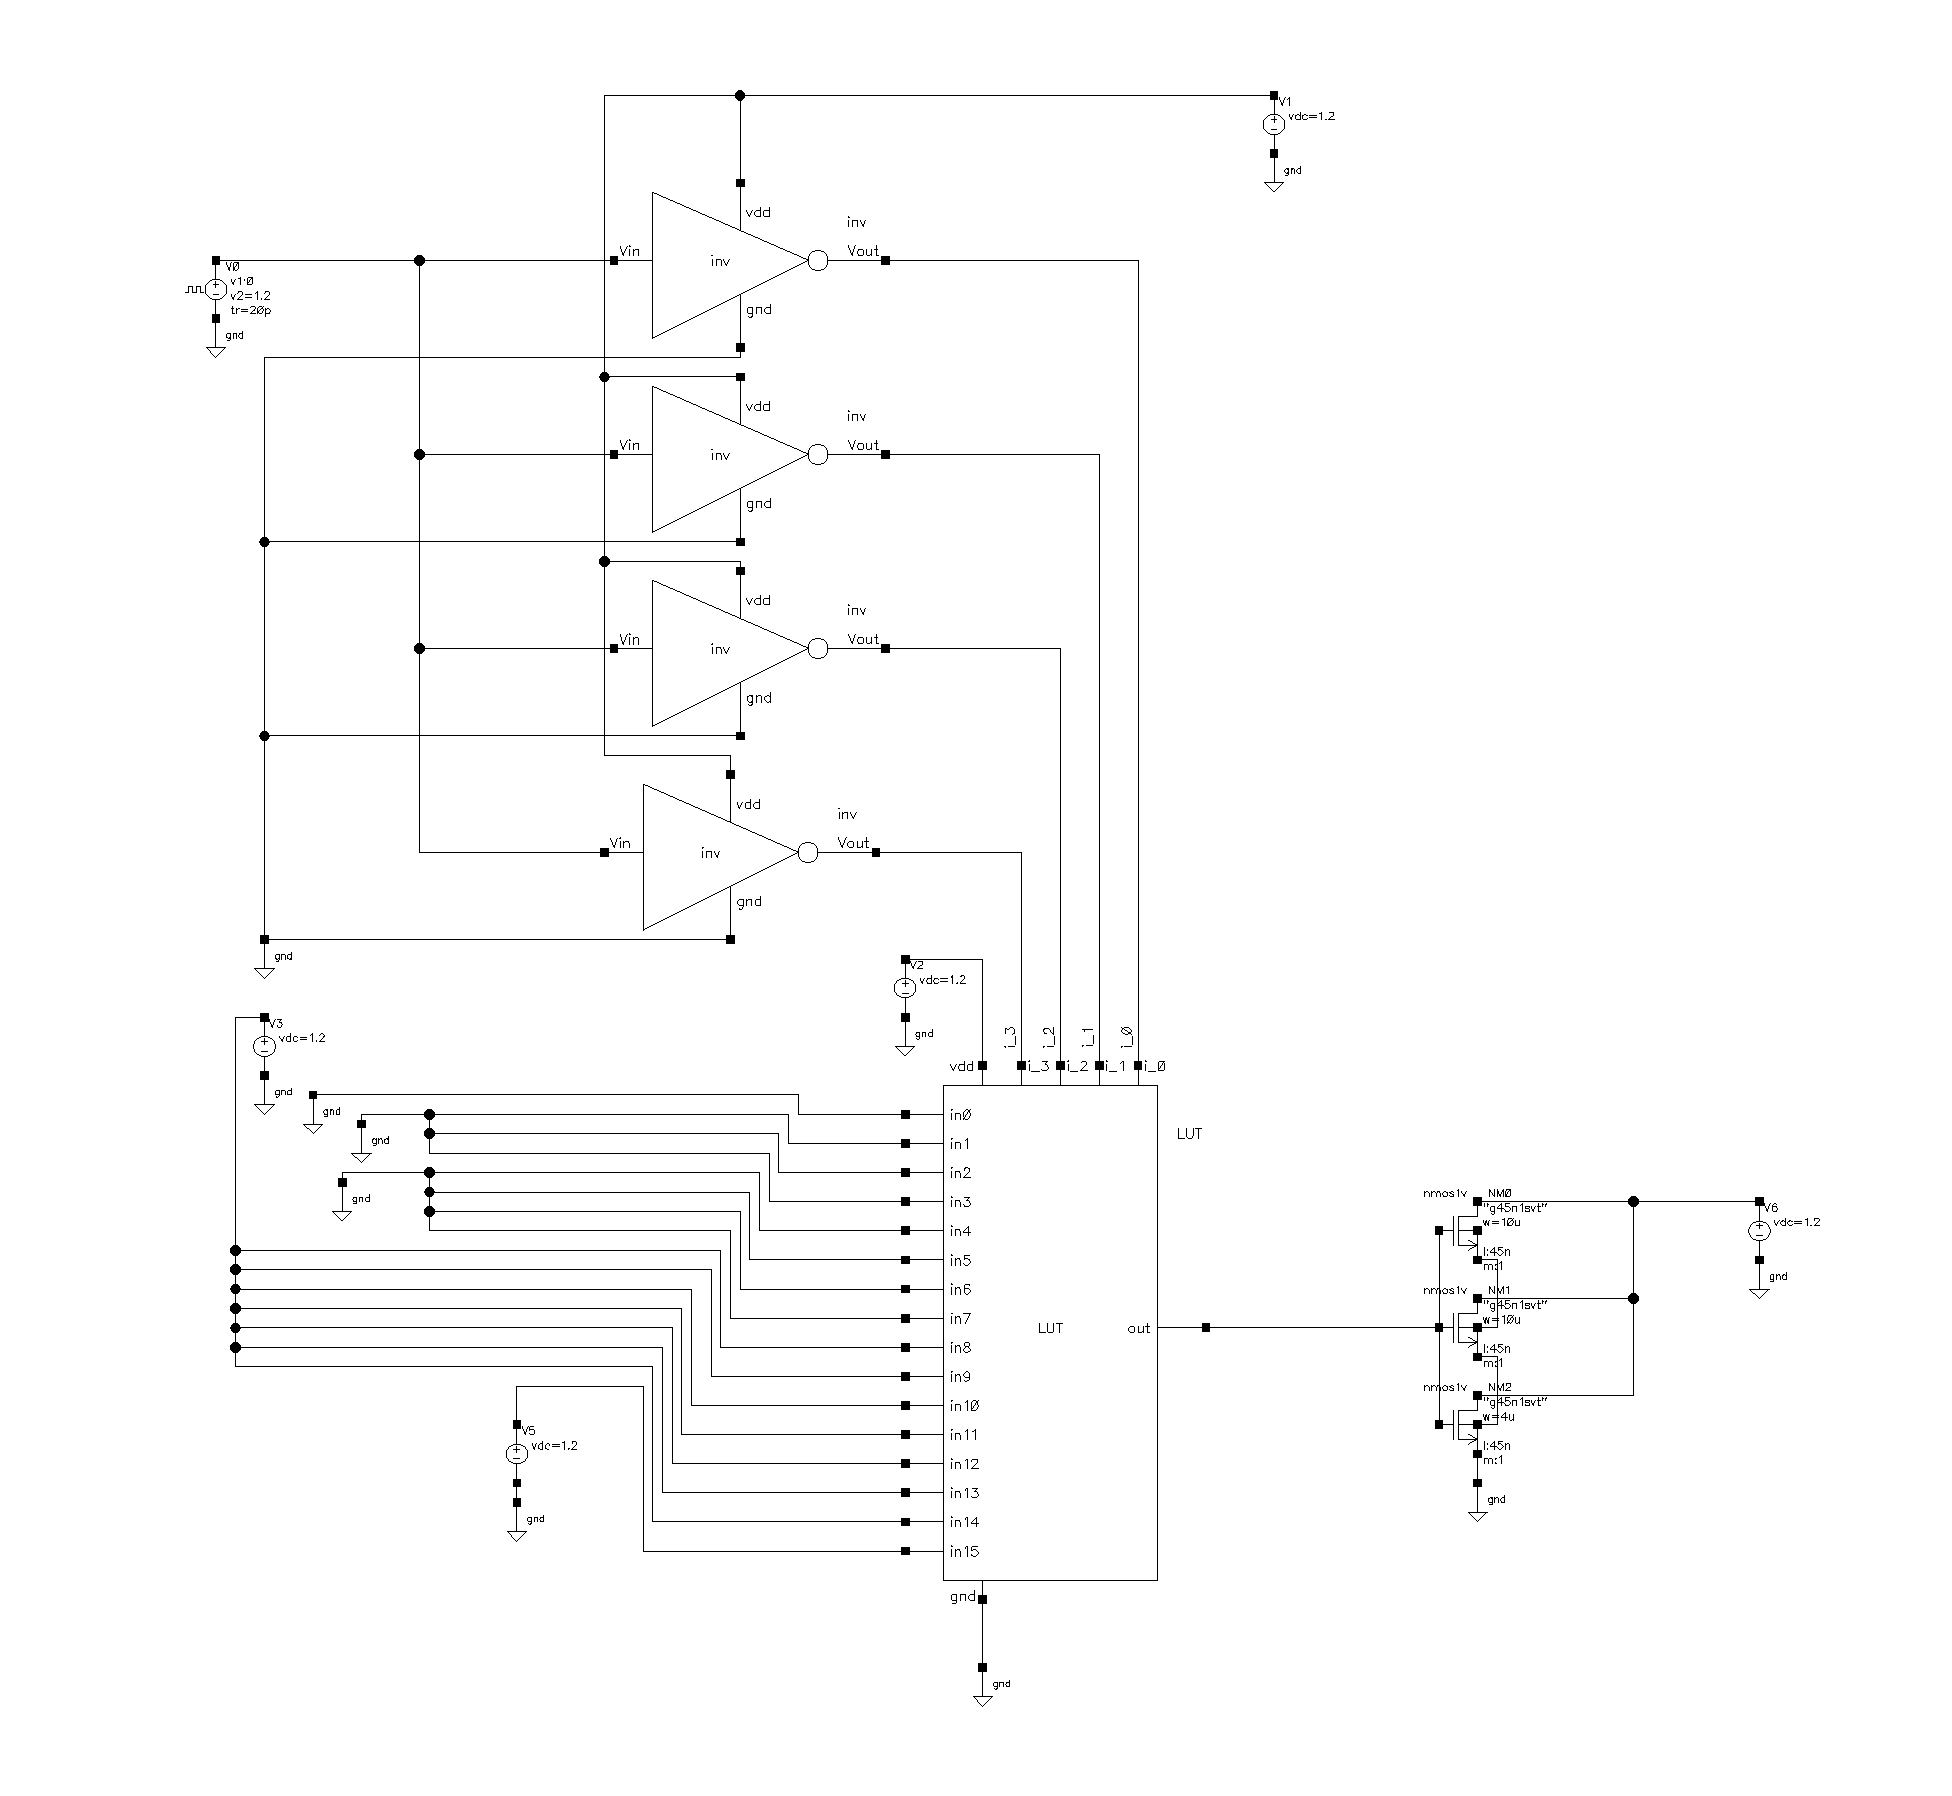
\includegraphics[width=0.8\linewidth]{writeup//figures/lut_delay_testbench.png}
    \caption{}
\end{figure}

In this test configuration, the first eight data inputs of the 16:1 LUT (\texttt{data<7:0>}) are tied to ground, while the remaining eight inputs (\texttt{data<15:8>}) are tied to $V_{DD}$. This data pattern mirrors the configuration used in the baseline delay measurement, as the same testbench was specified for the frequency analysis to ensure consistency across design metrics. The address inputs (\texttt{addr<3:0>}) are driven by pulse sources, each passing through a minimum-sized inverter chain to model realistic input loading and transition characteristics. To evaluate the frequency response of the LUT, the input pulse frequency was parameterized using a design variable $f$, enabling a parametric sweep across a range of operating frequencies. This setup allowed systematic identification of the maximum input frequency at which the LUT output remains functionally correct before timing violations or logic errors occur due to insufficient propagation time through the MUX network.


\newpage

\subsection{Simulation Results and Metric Value}

\begin{figure}[H]
    \centering
    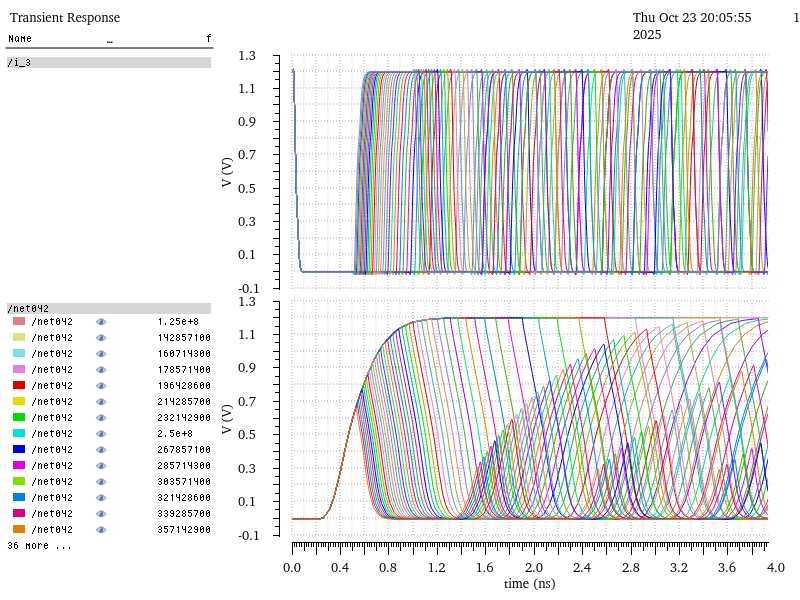
\includegraphics[width=\linewidth]{writeup//figures/frequency_response_param.png}
    \caption{Frequency response at output of the buffer stage}
\end{figure}

The parametric sweep of the input frequency from 125~MHz to 2~GHz produced the transient response shown in Fig. 14. As observed, the output waveforms initially exhibit transient behavior before reaching steady-state operation. This response corresponds to the early portion of the simulation, where switching activity and internal node voltages are still stabilizing across the multiple MUX stages. After several cycles, the transient effects subside and the circuit transitions to a periodic steady-state. Since accurate frequency characterization requires analysis under stable operating conditions, only the steady-state portion of the response was considered for extracting the maximum operating frequency, as presented in the following figure.

\begin{figure}[H]
    \centering
    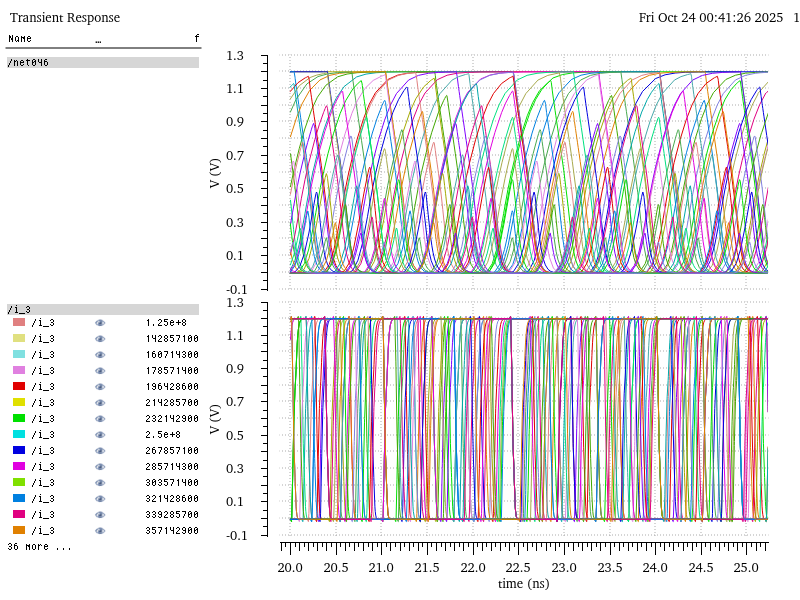
\includegraphics[width=\linewidth]{writeup//figures/frequency_response_param_20_40.png}
    \caption{Frequency response at output of the buffer stage}
\end{figure}

The steady-state response of the LUT output for the same frequency sweep range (125~MHz to 2~GHz) is shown in Fig. 15. After the initial transient period, the input and output signals exhibit periodic behavior, allowing for accurate assessment of the circuit’s frequency limits. Each colored trace corresponds to a different input frequency used in the parametric sweep, illustrating how the output waveform integrity degrades progressively as the frequency approaches the upper limit of reliable operation. These results form the basis for determining the maximum operating frequency at which the LUT maintains correct logical functionality across all address transitions.

\begin{figure}[H]
    \centering
    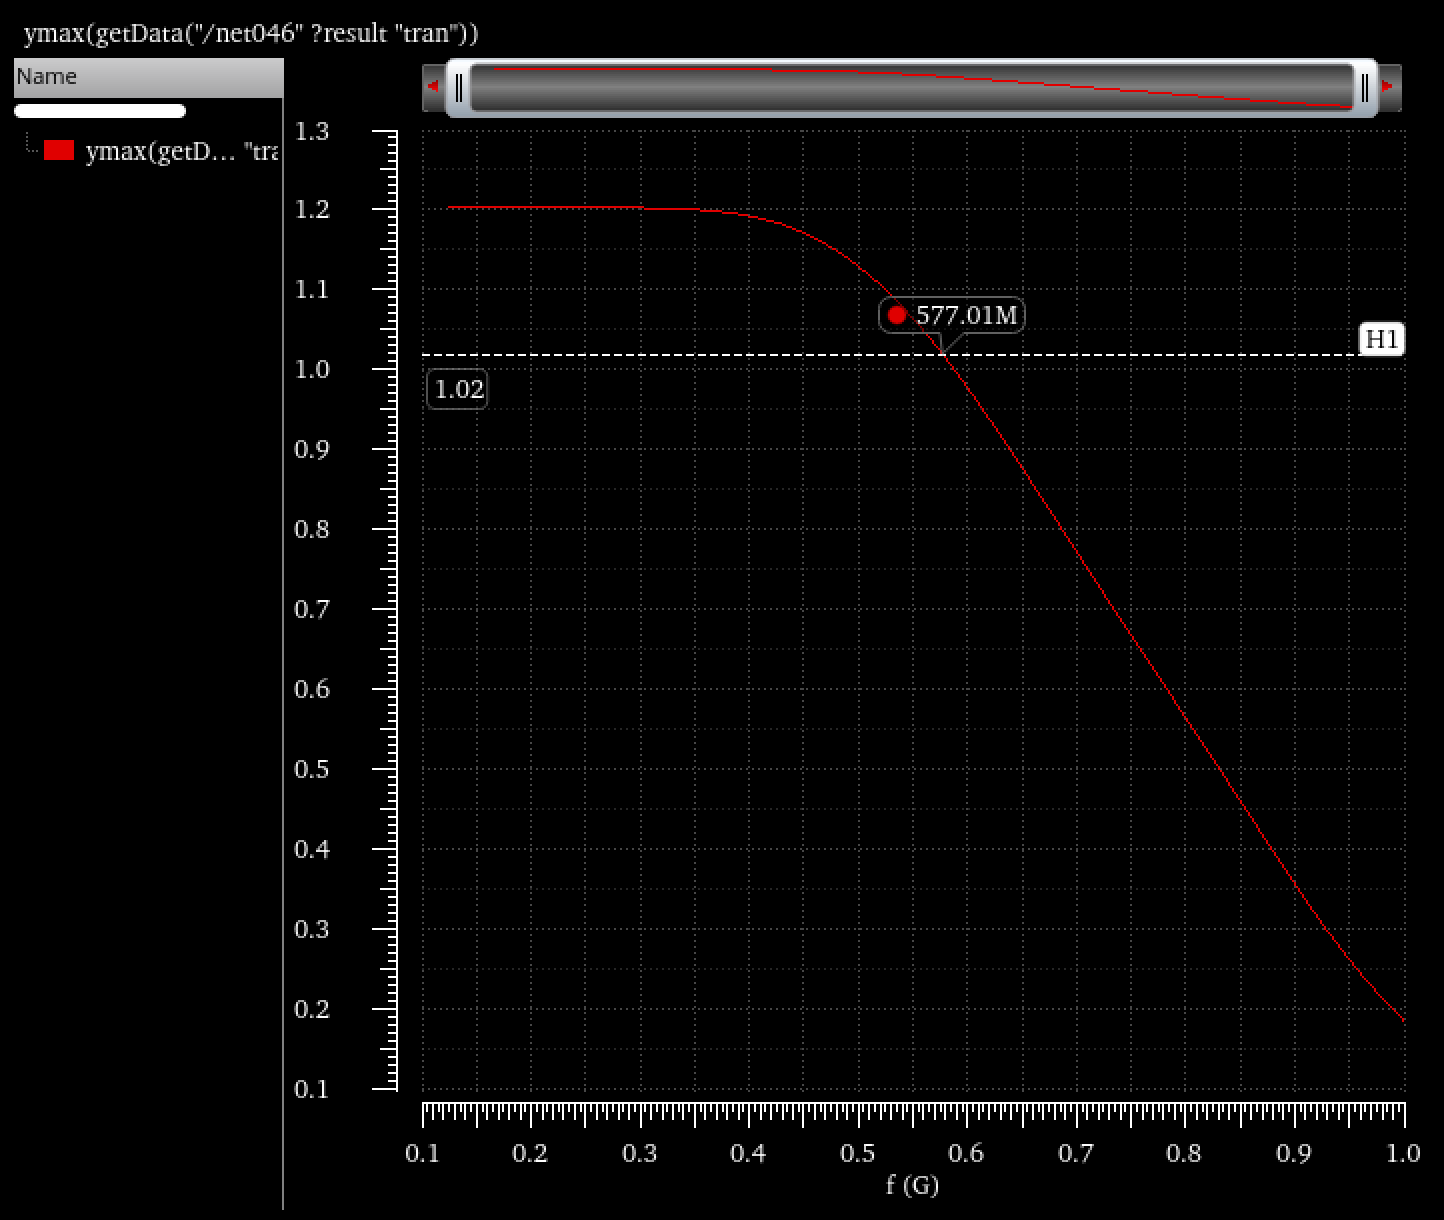
\includegraphics[width=\linewidth]{writeup//figures/max_frequencies.png}
    \caption{Extracting frequency value that allows for 85\% of VDD after buffer stage}
\end{figure}

From the steady-state frequency response, the peak output voltage at the buffer stage was recorded for each simulated frequency value. These maximum values were then plotted as shown in Fig. 16 to determine the point at which the output amplitude drops below an acceptable threshold. The cutoff criterion was defined as 85\% of $V_{DD}$ (i.e., 1.02~V for $V_{DD}=1.2$~V), corresponding to the minimum logic-high level that still ensures reliable digital operation. Based on this criterion, the maximum operating frequency of the baseline LUT was extracted to be approximately \textbf{577~MHz}. Beyond this frequency, the output fails to reach valid logic levels due to insufficient charging and discharging time within the MUX hierarchy and the output buffer.

\newpage

% ------------------ SECTION 5 ------------------
\section{Baseline Energy Measurement}
\subsection{Test Schematic}

\begin{figure}[H]
    \centering
    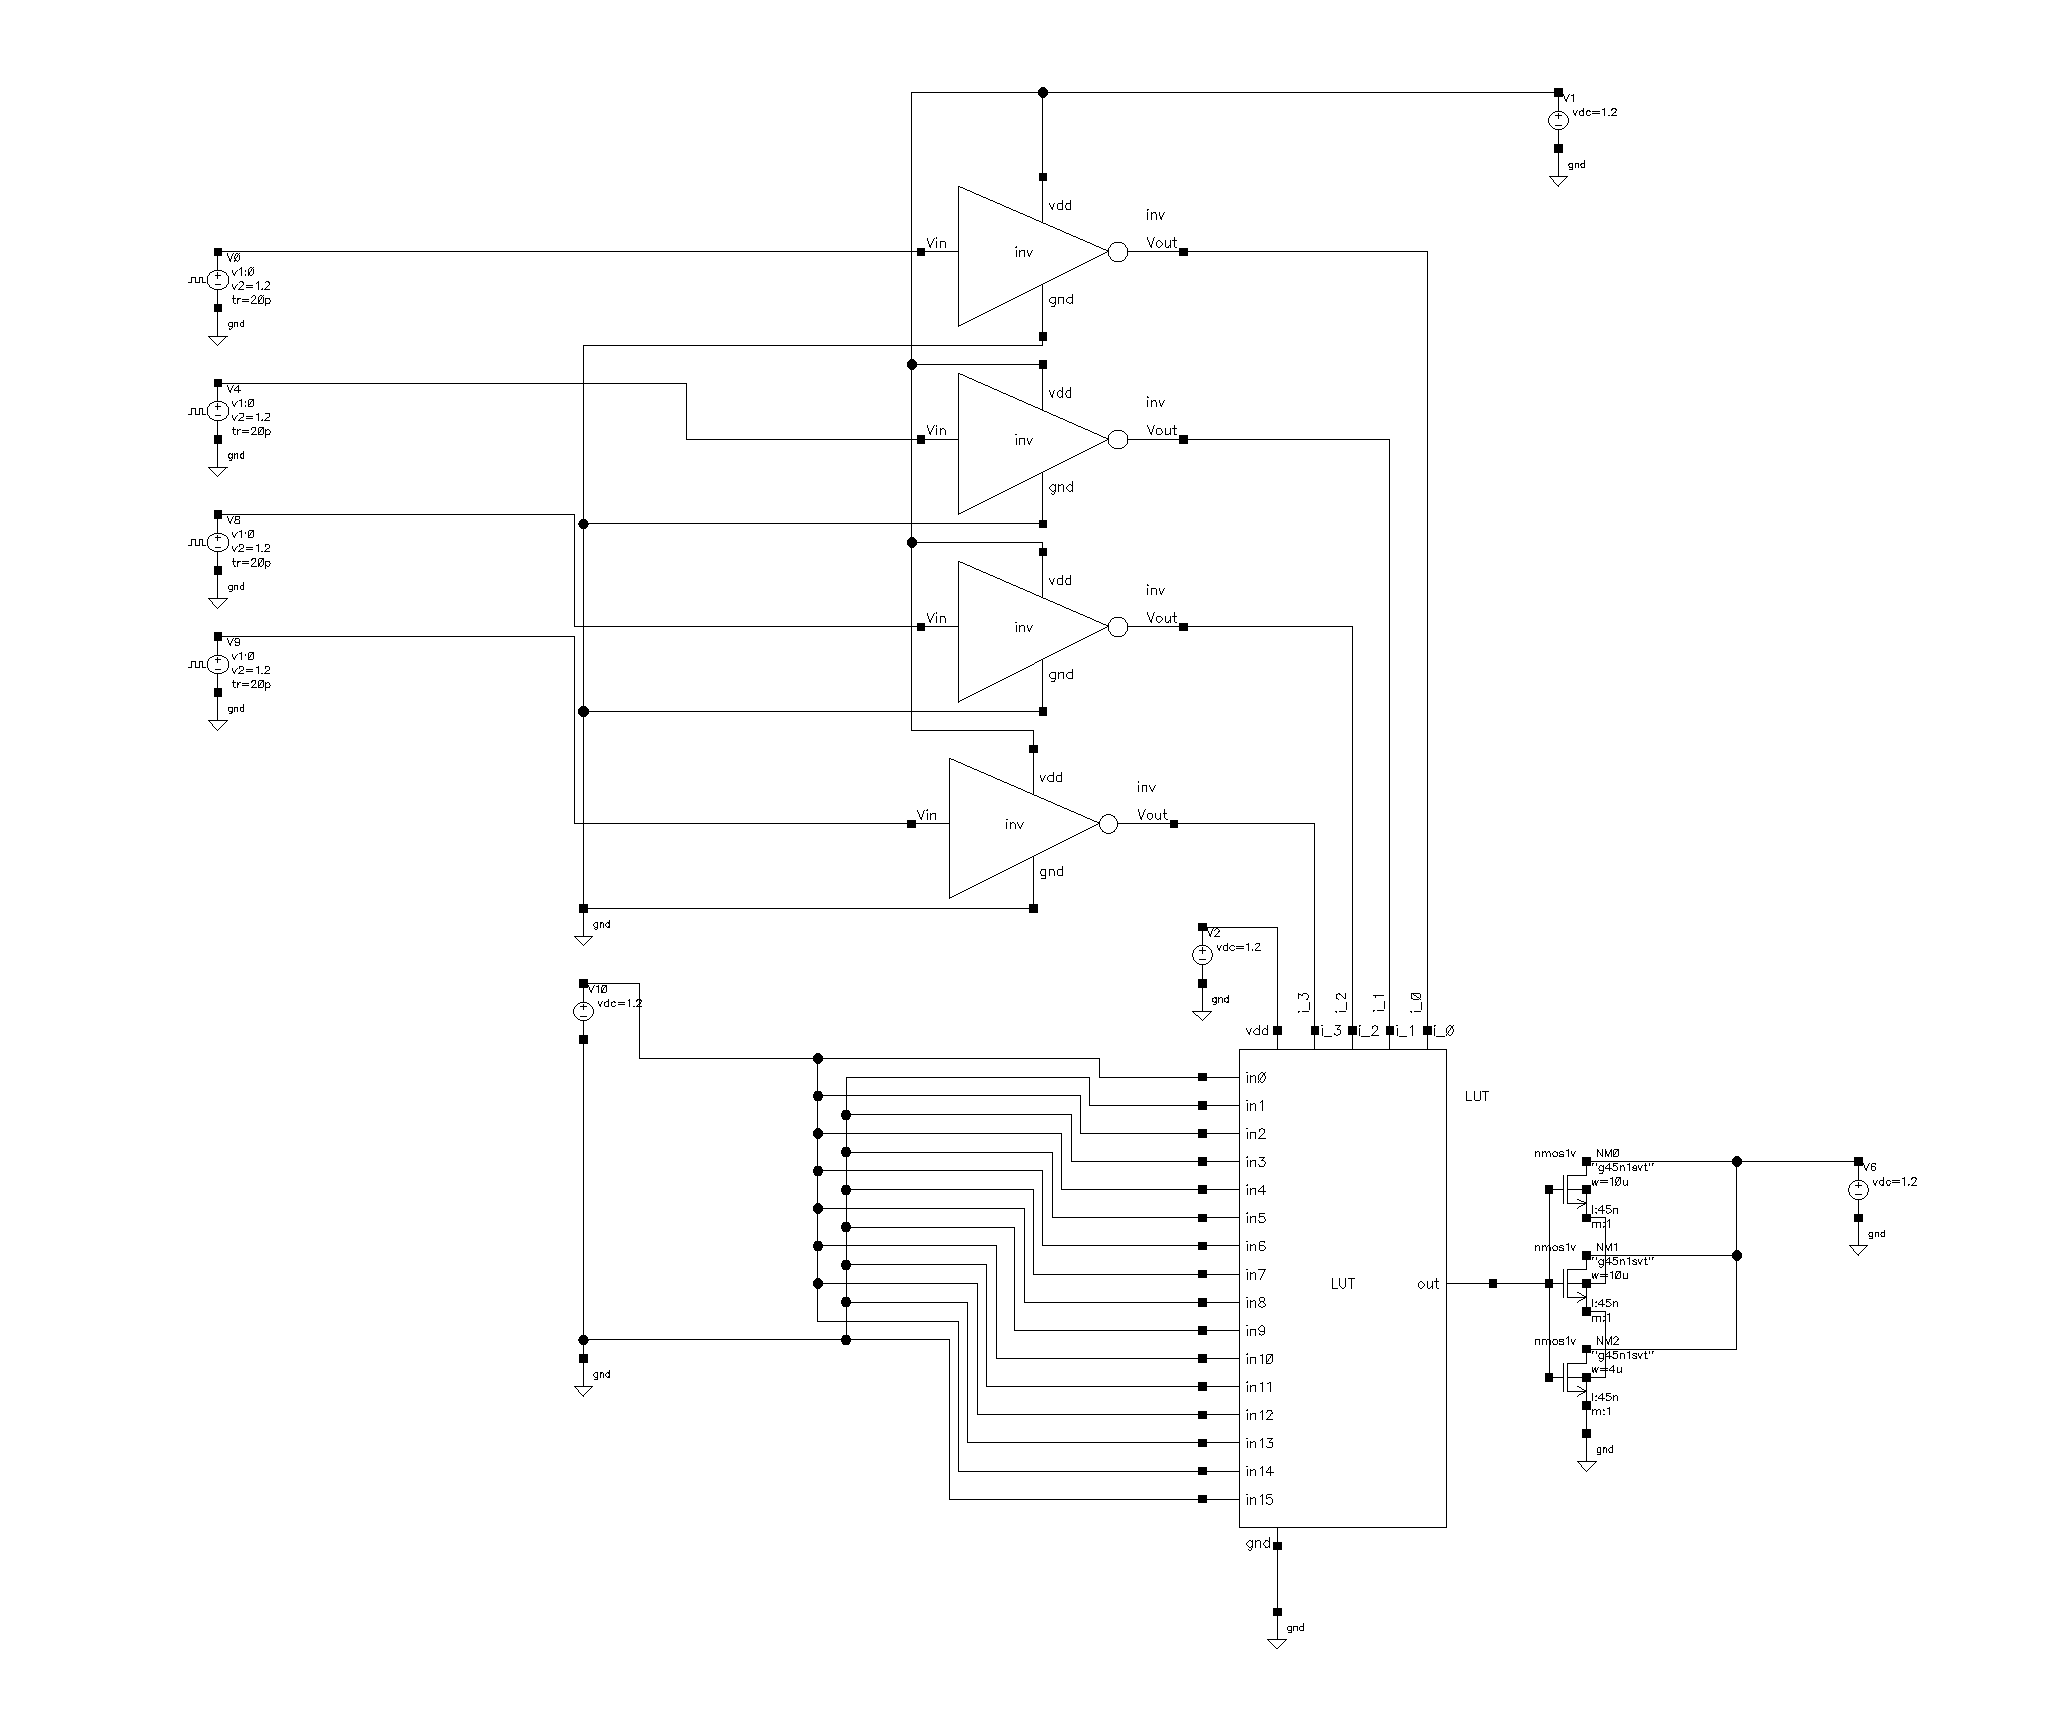
\includegraphics[width=\linewidth]{writeup//figures/lut_energy_testbench.png}
    \caption{}
\end{figure}

Individual \texttt{Vpulse} sources were used to supply the driving inverters for the address lines in order to support our measurmeent test case. To accurately measure the total active energy, a separate supply source was used for the device under test (the LUT) and for its output buffer. The instantaneous current through the LUT’s dedicated $V_{DD}$ source was monitored to capture the dynamic current drawn by the internal MUX hierarchy, while the current at the LUT output node was simultaneously measured to account for current flow through the pass transistors in the 2:1 MUX network. The total energy consumption was then obtained by integrating these current measurements over one complete address cycle.

\newpage

\subsection{Test Case}

\begin{figure}[H]
    \centering
    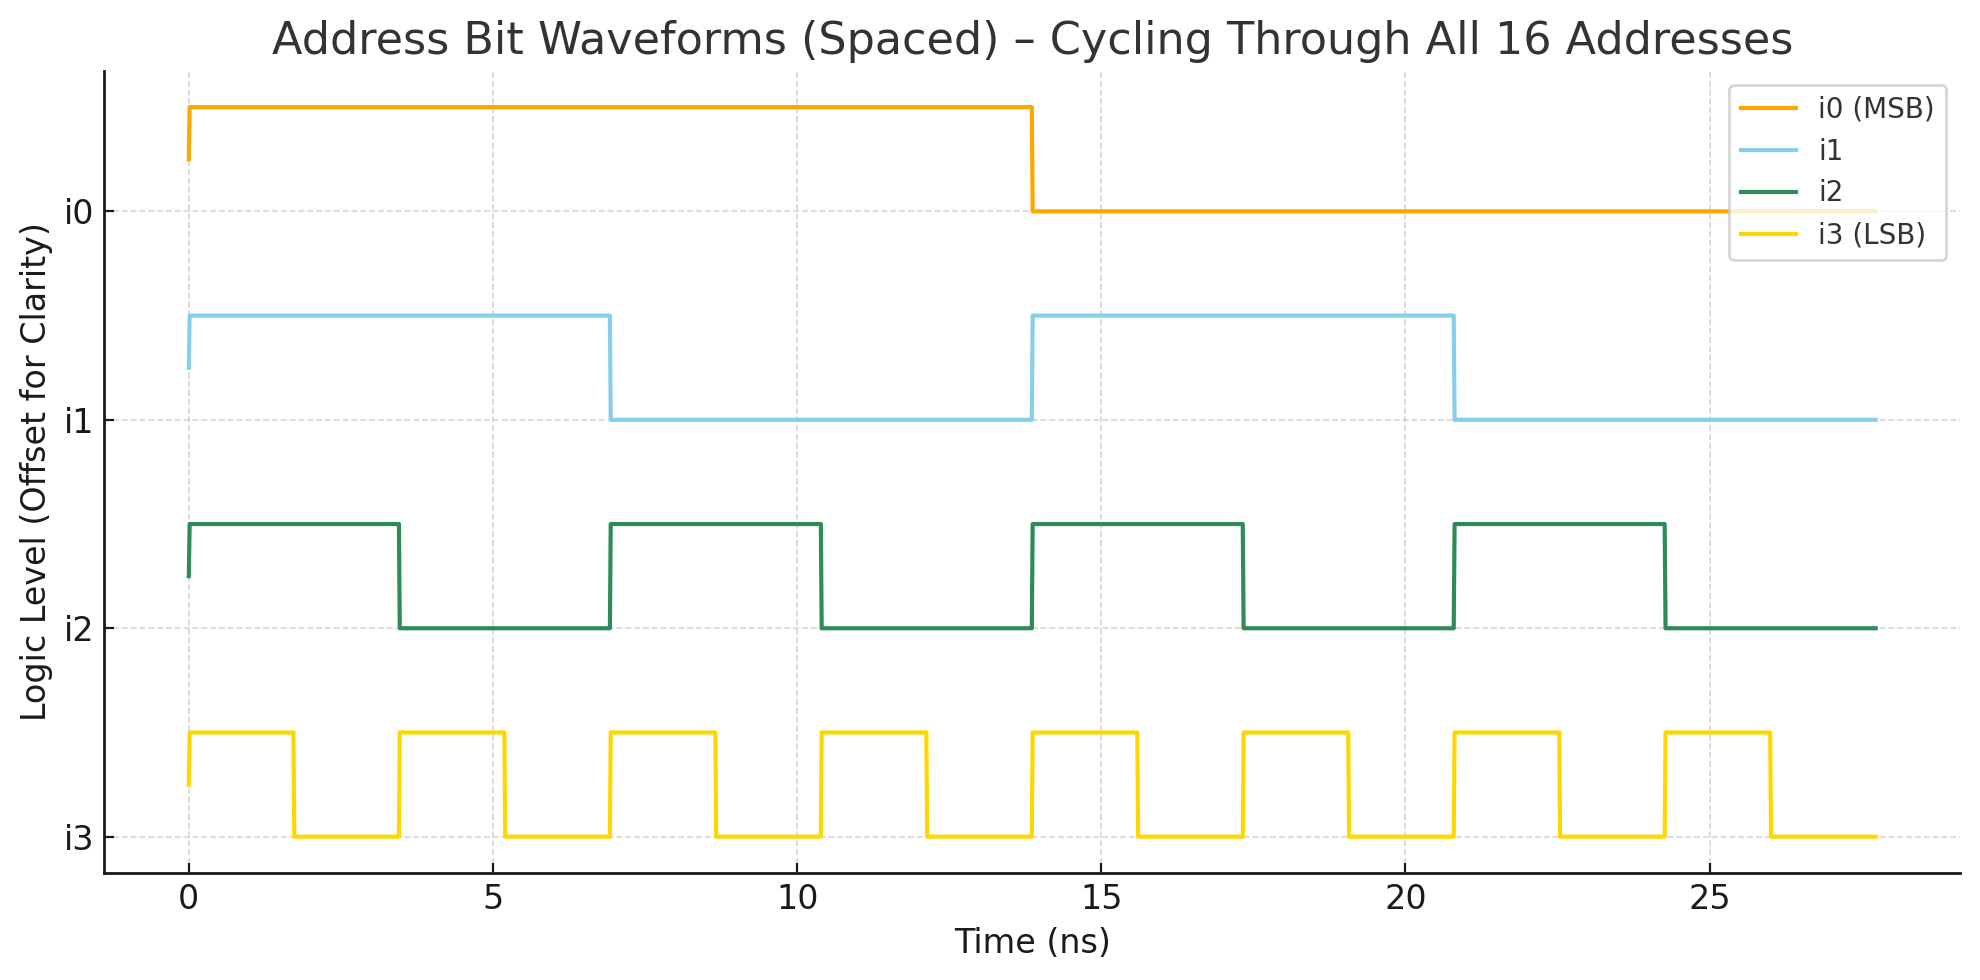
\includegraphics[width=\linewidth]{writeup//figures/input_case_energy.png}
    \caption{}
\end{figure}

The baseline energy measurement testbench is configured to exercise all address combinations of the 16:1 LUT once per simulation cycle. The address inputs are defined such that \texttt{i\_3} serves as the least significant bit (LSB) and \texttt{i\_0} as the most significant bit (MSB). The MSB is driven with a period of $16T$, while the LSB is driven with a period of $2T$, where $T = \frac{1}{577{,}010{,}000}$~s corresponds to the maximum operating frequency determined from the frequency analysis. This timing relationship ensures that the four address inputs sequentially toggle through all $2^4 = 16$ possible address states exactly once per full simulation period.

\newpage

\subsection{Simulation Results and Metric Value}
\begin{figure}[H]
    \centering
    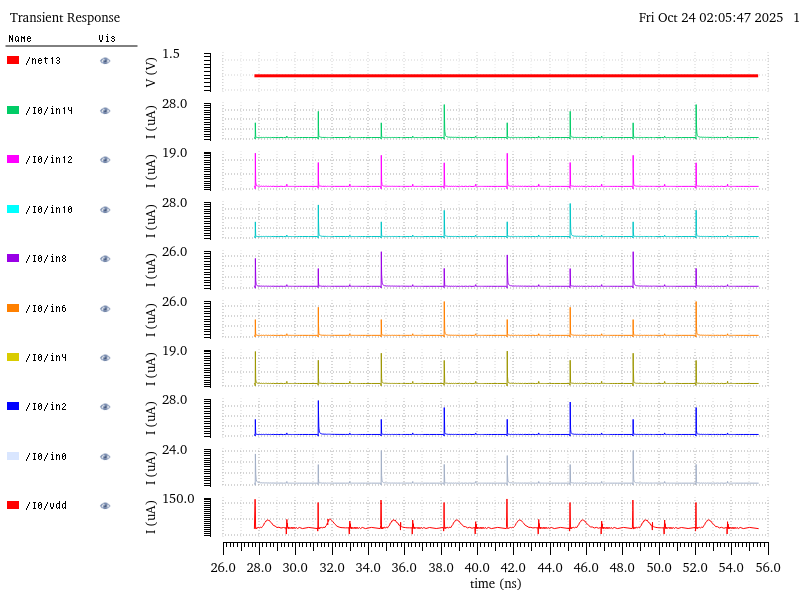
\includegraphics[width=0.7\linewidth]{writeup//figures/baseline_energy_currents.png}
    \caption{}
\end{figure}

\begin{figure}[H]
    \centering
    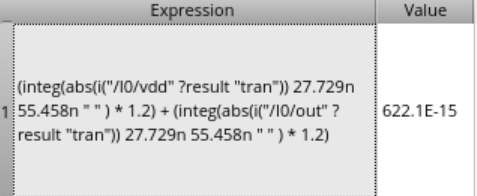
\includegraphics[width=0.4\linewidth]{writeup//figures/baseline_energy_val.png}
    \caption{}
\end{figure}

The transient current waveforms in Fig. 19 show the instantaneous current drawn from the LUT’s dedicated $V_{DD}$ source (top) and the output node (bottom) as the address inputs cycle through all 16 possible states at the maximum operating frequency. The $V_{DD}$ current spikes correspond to charging events within the internal pass-transistor network and the output buffer, while the output current captures transient discharge and charge paths through the 2:1 MUX structure.  

To calculate the total active energy, both current waveforms were integrated over one full address cycle and multiplied by $V_{DD} = 1.2~\text{V}$. The resulting energy consumption of the baseline LUT was found to be $\boxed{E_{\text{baseline}} = 622.1~\text{fJ}}$.

This value represents the total dynamic energy required for one complete traversal of all address combinations, accounting for switching losses in both the MUX array and the output buffer. The magnitude of this value reflects the cumulative capacitive charging and discharging activity across the hierarchical MUX network under maximum-frequency operation.

\newpage

% ------------------ SECTION 6 ------------------
\section{Optimized Design}
\subsection{Optimized Design Schematics}

\subsubsection*{Inverters (Buffer Inverter kept at Minsize)}

\begin{figure}[H]
    \centering
    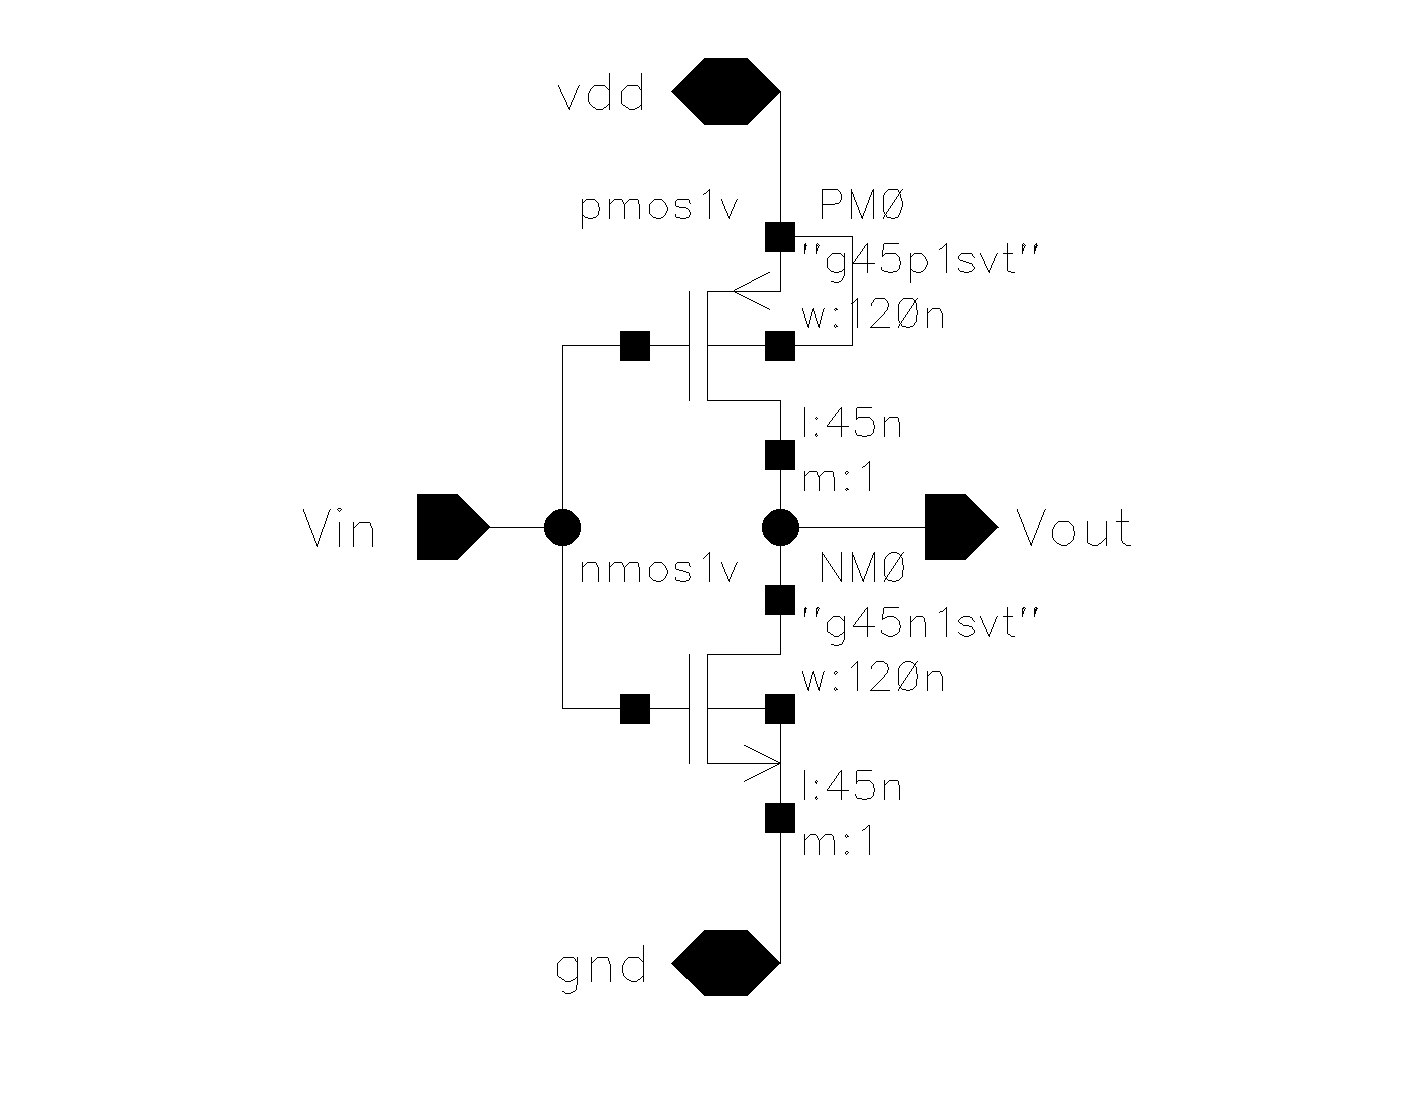
\includegraphics[width=0.6\linewidth]{writeup//figures/inv_sch.png}
    \caption{}
\end{figure}

\subsubsection*{Symbol}

\begin{figure}[H]
    \centering
    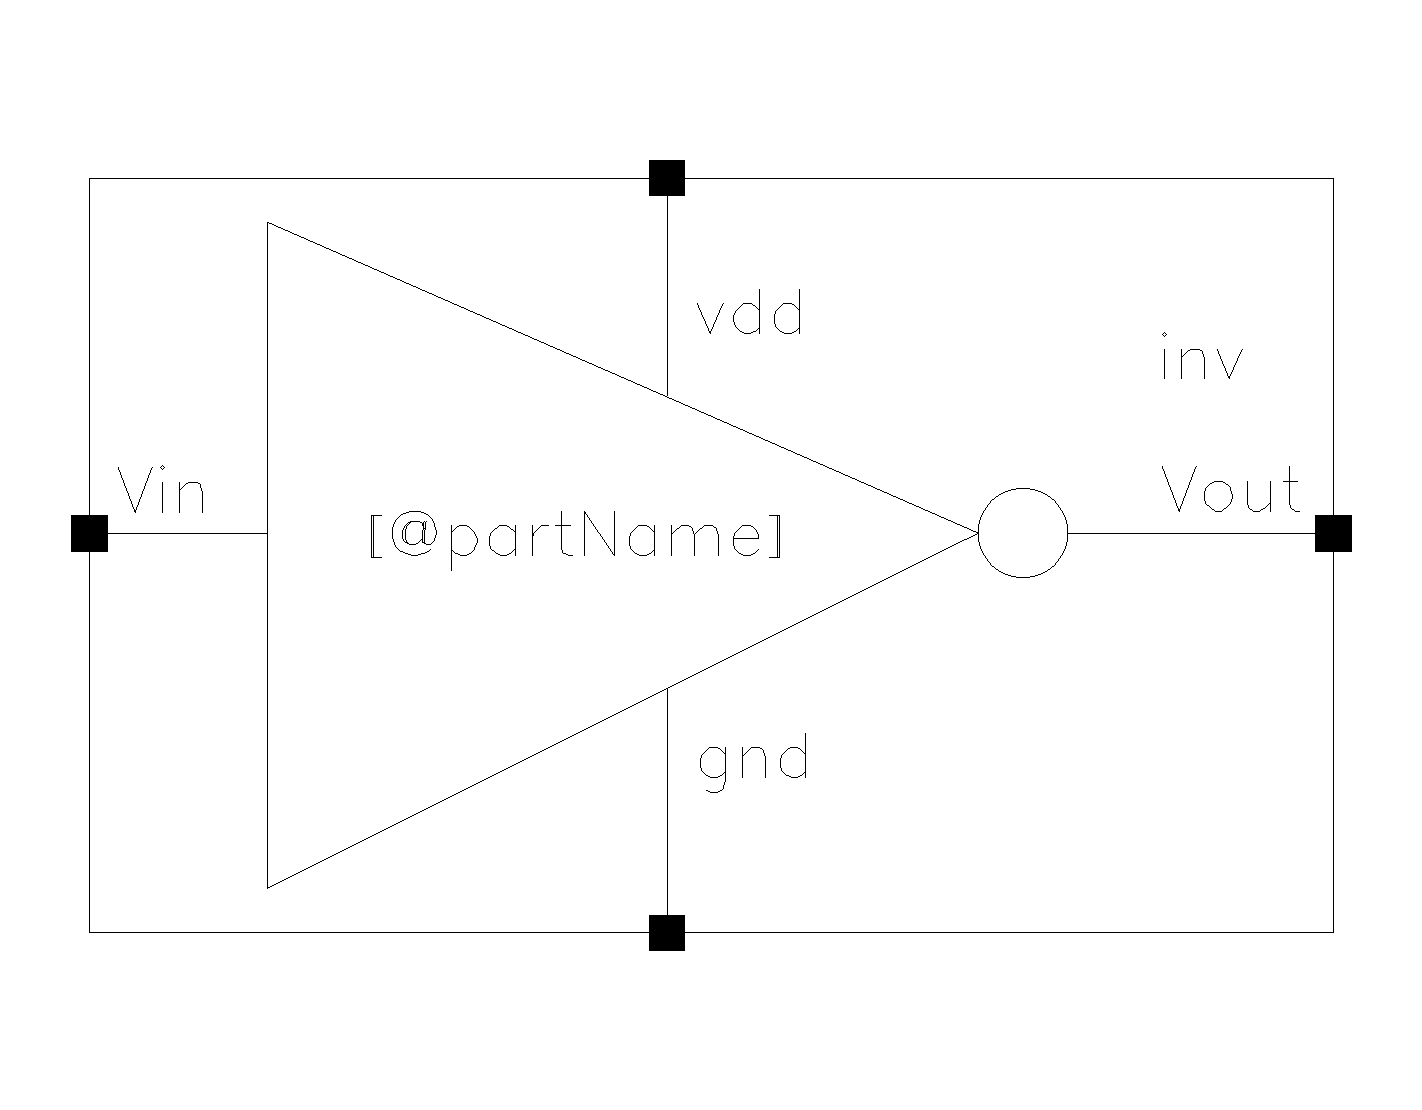
\includegraphics[width=0.6\linewidth]{writeup//figures/inv_sym.png}
    \caption{}
\end{figure}

\subsubsection*{2:1 MUX Optimized Schematics}

\begin{figure}[H]
    \centering
    % Subfigure A
    \begin{subfigure}[b]{0.48\textwidth}
        \centering
        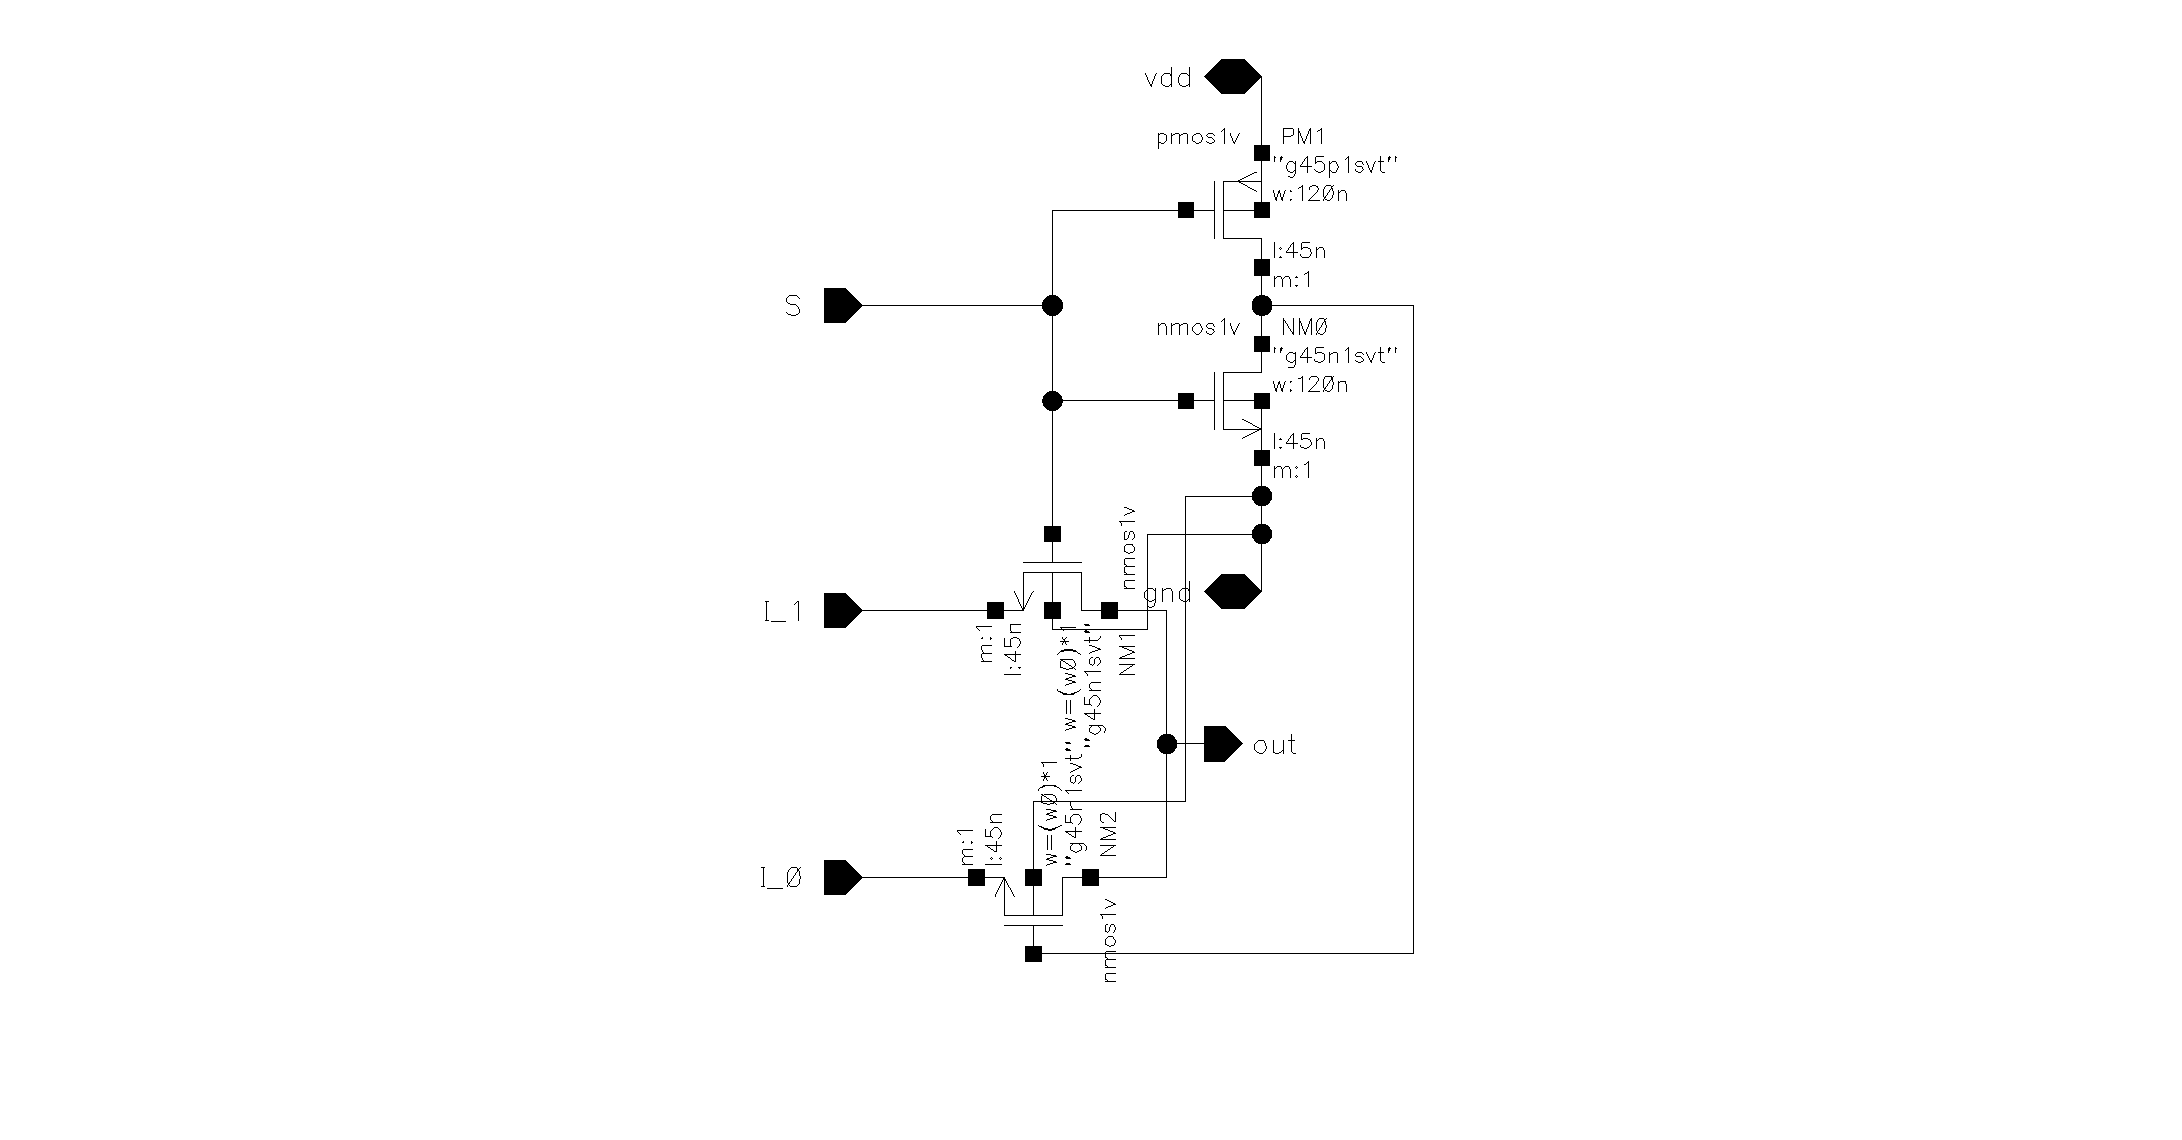
\includegraphics[width=\textwidth]{writeup/figures/mux_w0_opt.png}
        \caption{}
        \label{fig:mux_w0_opt}
    \end{subfigure}
    \hfill
    % Subfigure B
    \begin{subfigure}[b]{0.48\textwidth}
        \centering
        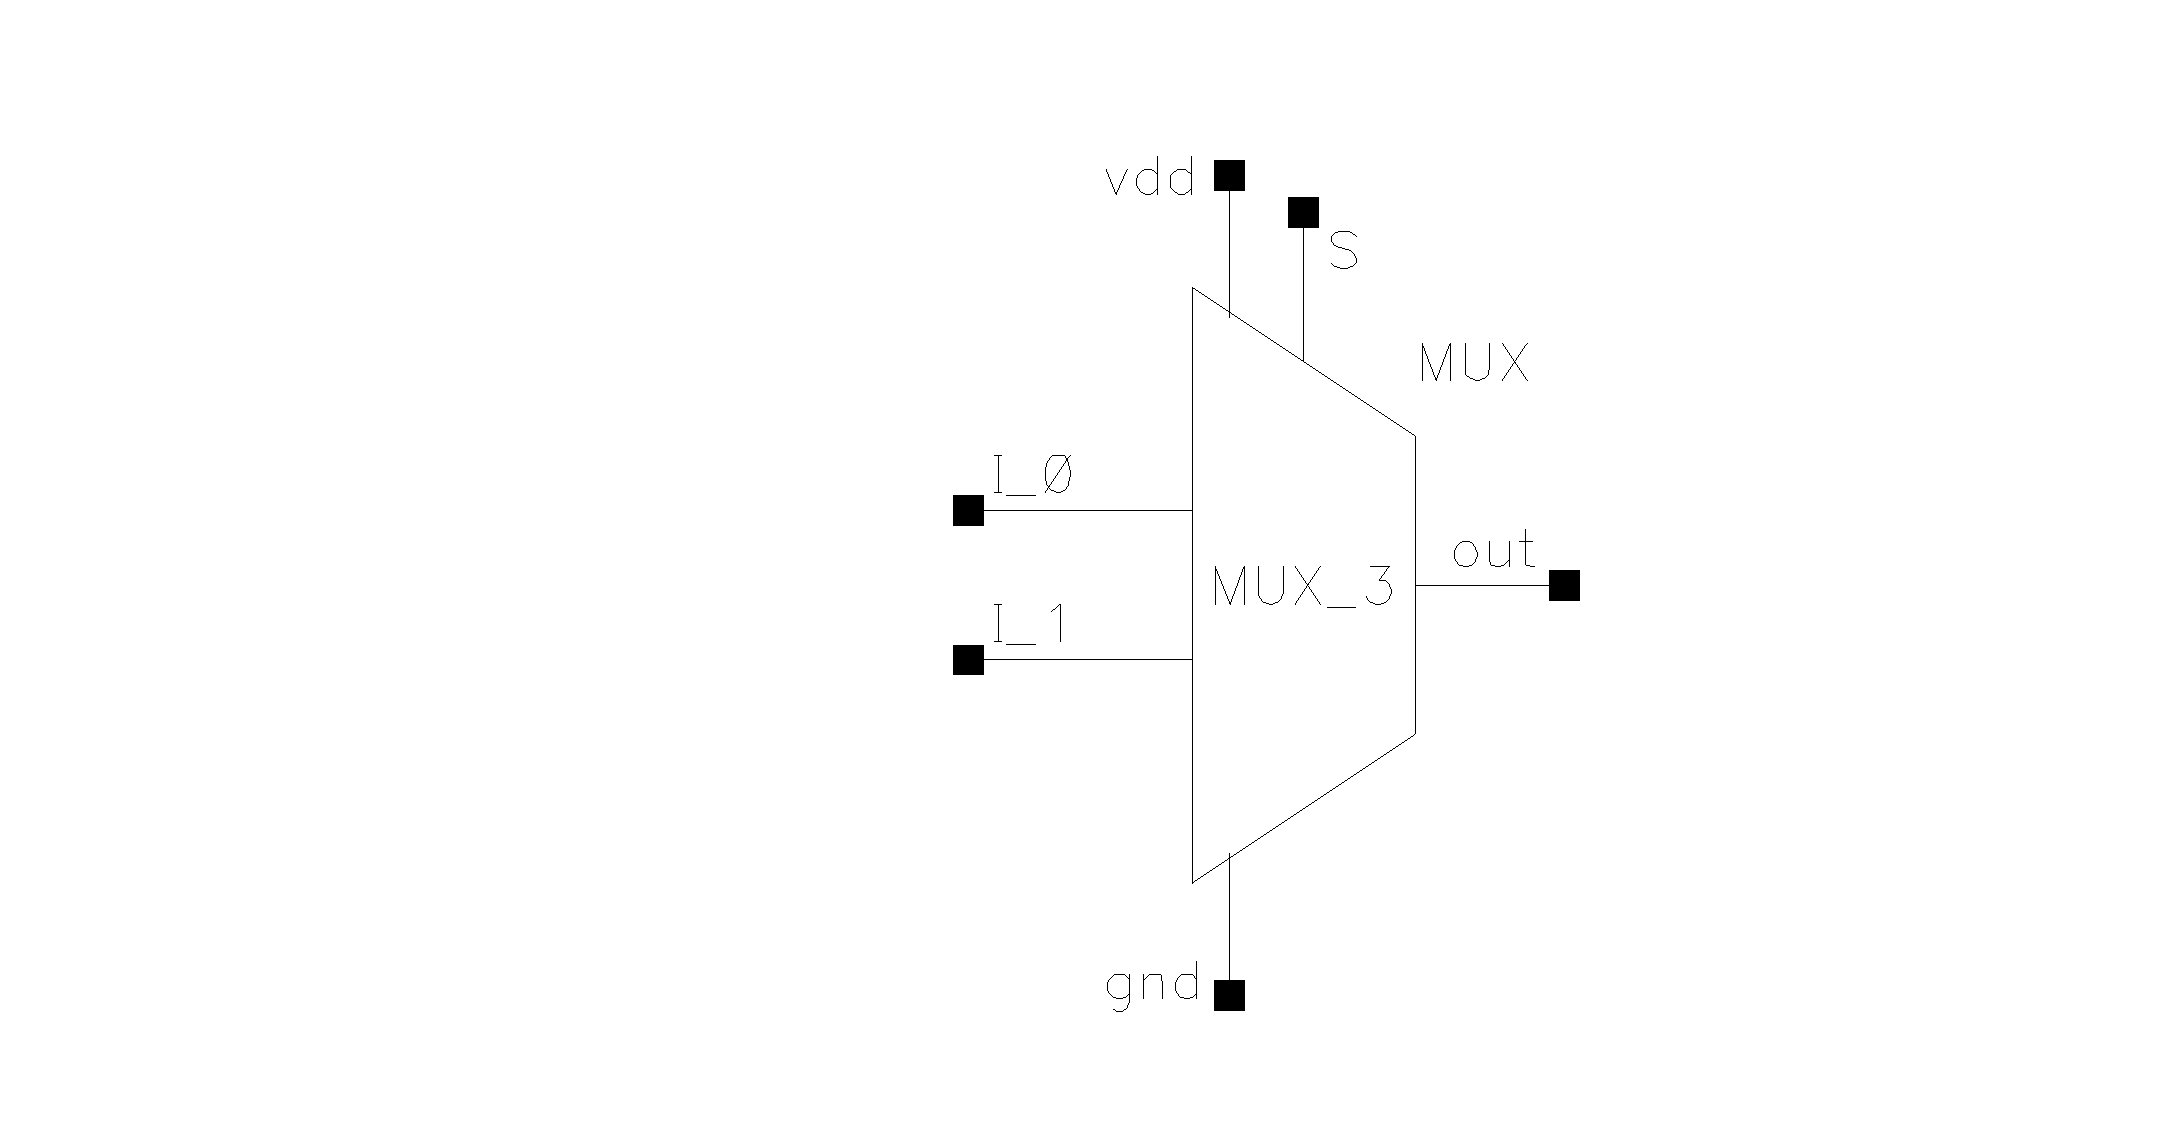
\includegraphics[width=\textwidth]{writeup/figures/mux_w0_opt_sym.png}
        \caption{}
        \label{fig:mux_w0_opt_sym}
    \end{subfigure}
    \caption{Optimized MUX for first stage: schematic and its corresponding symbol}
    \label{fig:mux0_opt_comparison}
\end{figure}

\begin{figure}[H]
    \centering
    % Subfigure A
    \begin{subfigure}[b]{0.48\textwidth}
        \centering
        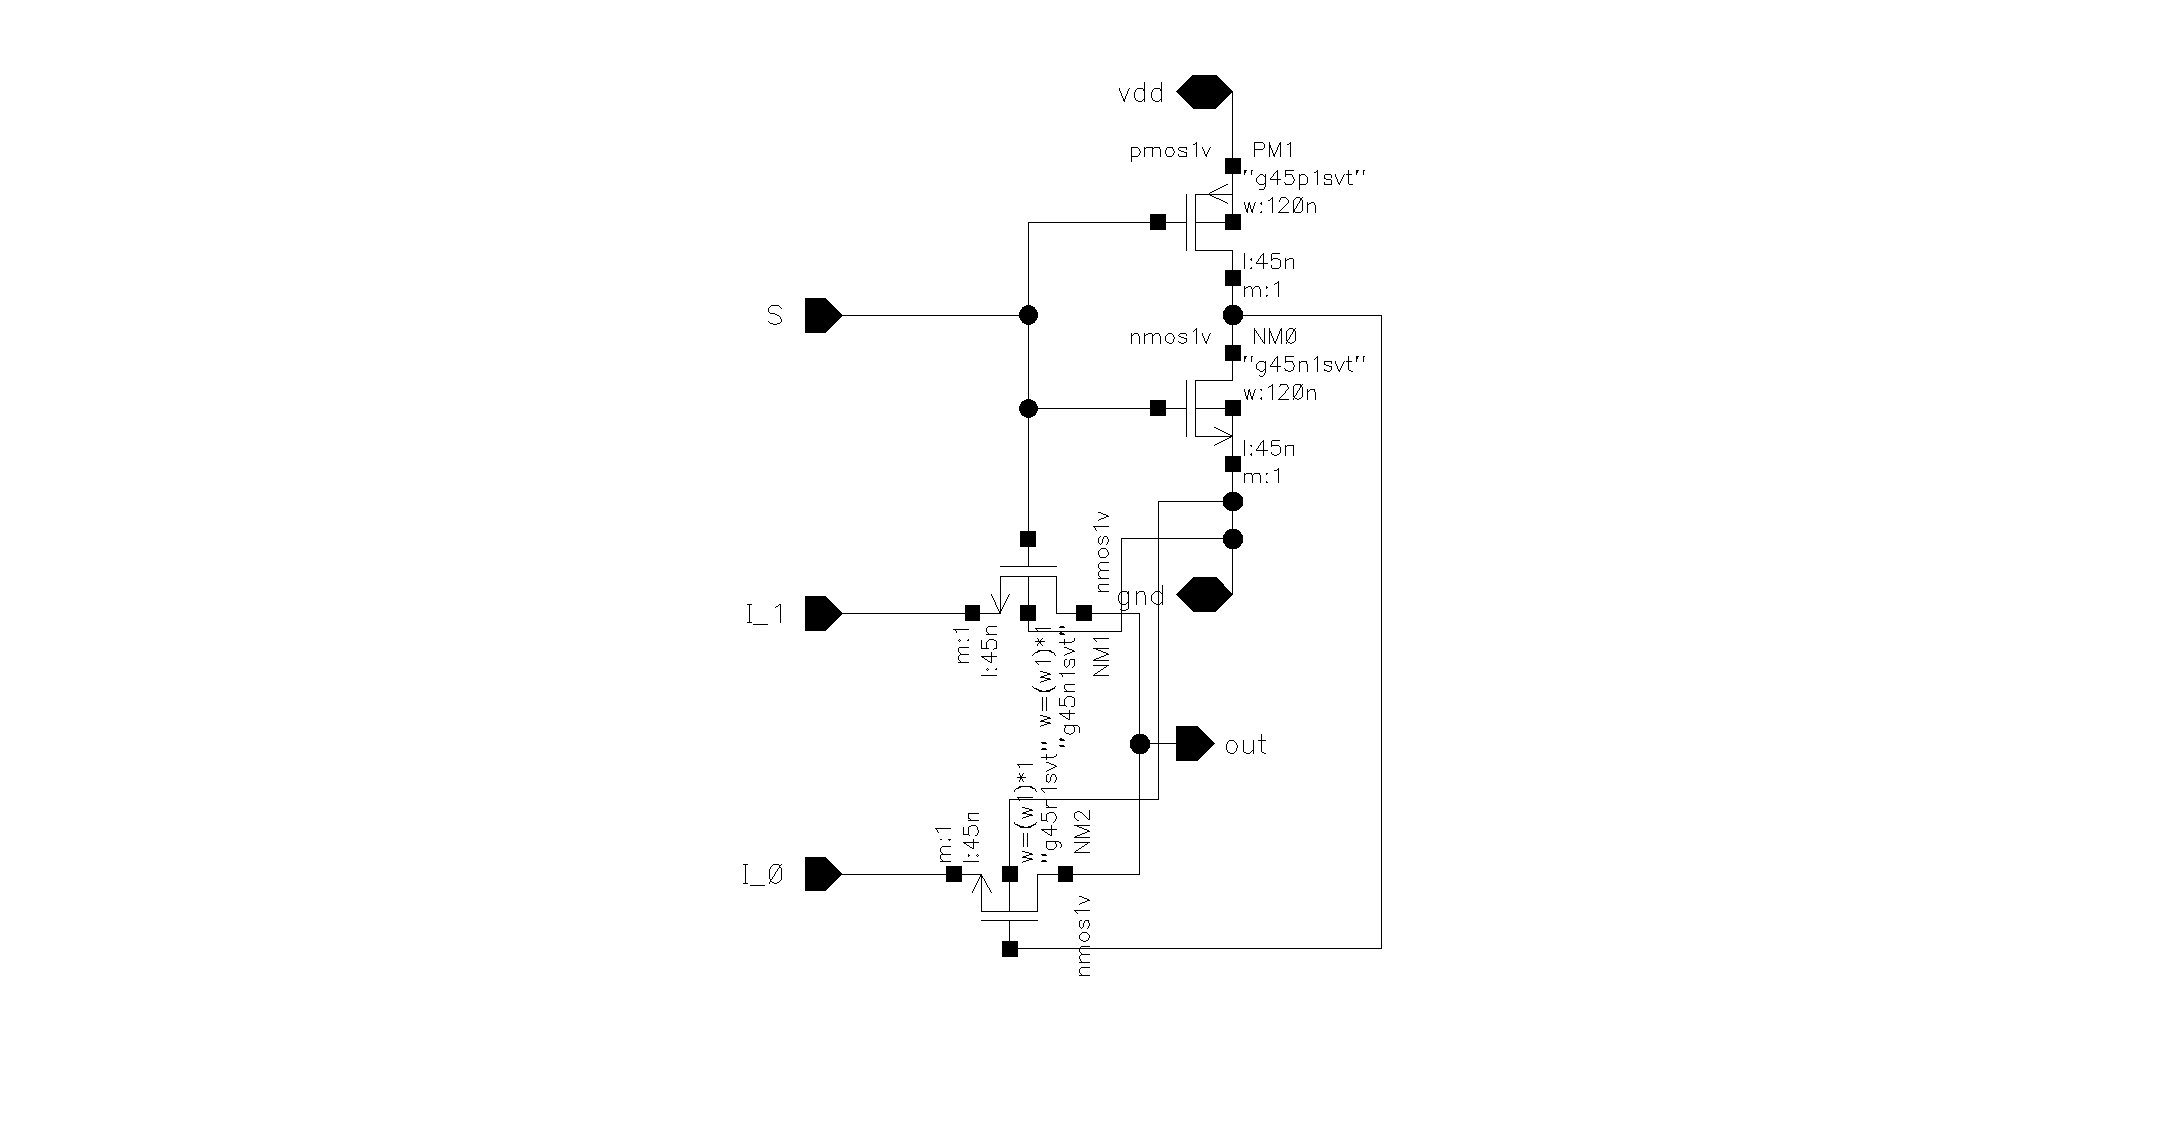
\includegraphics[width=\textwidth]{writeup/figures/mux_w1_opt.png}
        \caption{}
        \label{fig:mux_w1_opt}
    \end{subfigure}
    \hfill
    % Subfigure B
    \begin{subfigure}[b]{0.48\textwidth}
        \centering
        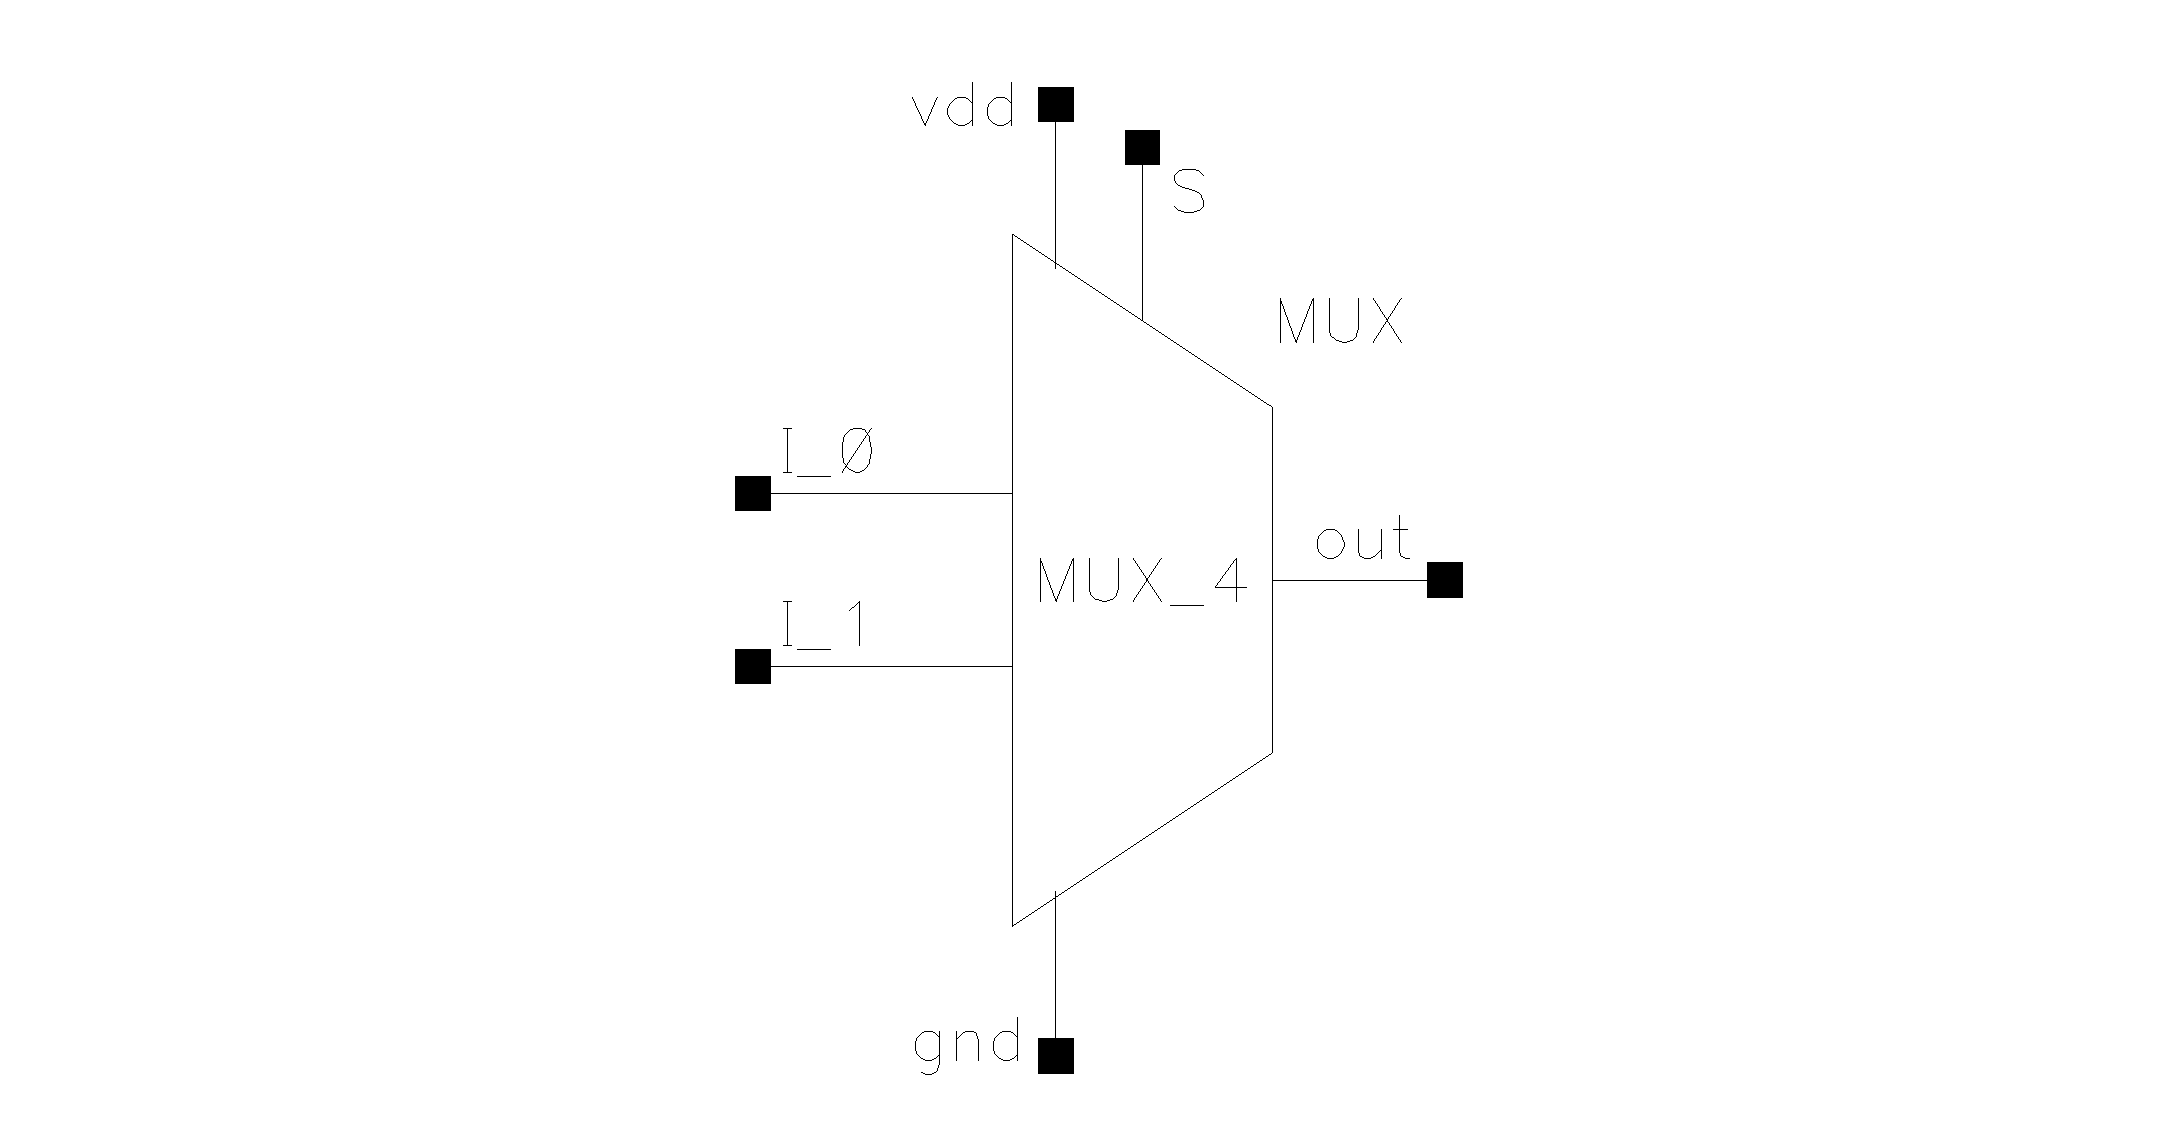
\includegraphics[width=\textwidth]{writeup/figures/mux_w1_opt_sym.png}
        \caption{}
        \label{fig:mux_w1_opt_sym}
    \end{subfigure}
    \caption{Optimized MUX for second stage: schematic and its corresponding symbol}
    \label{fig:mux1_opt_comparison}
\end{figure}

\begin{figure}[H]
    \centering
    % Subfigure A
    \begin{subfigure}[b]{0.48\textwidth}
        \centering
        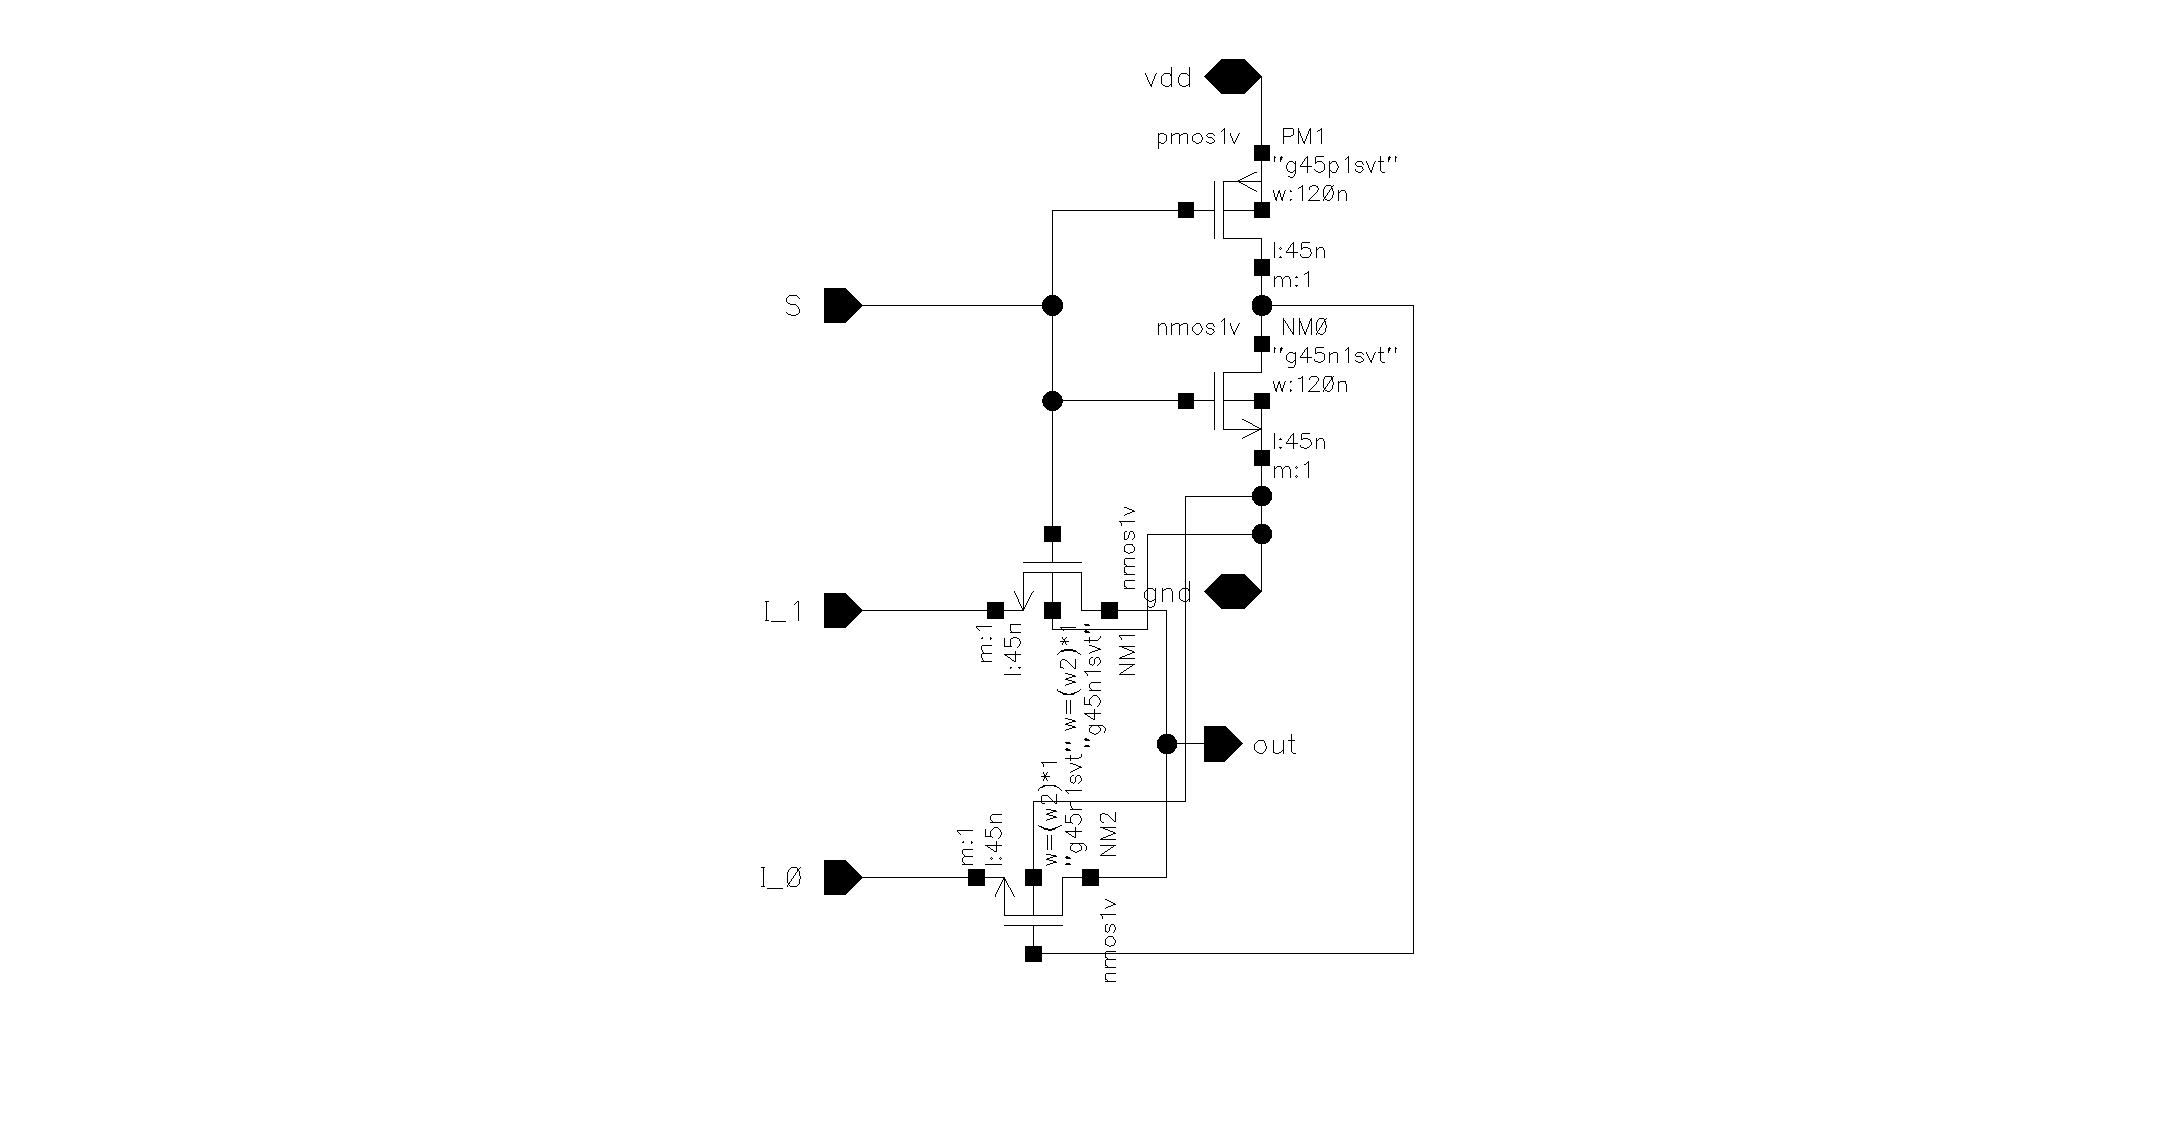
\includegraphics[width=\textwidth]{writeup/figures/mux_w2_opt.png}
        \caption{}
        \label{fig:mux_w2_opt}
    \end{subfigure}
    \hfill
    % Subfigure B
    \begin{subfigure}[b]{0.48\textwidth}
        \centering
        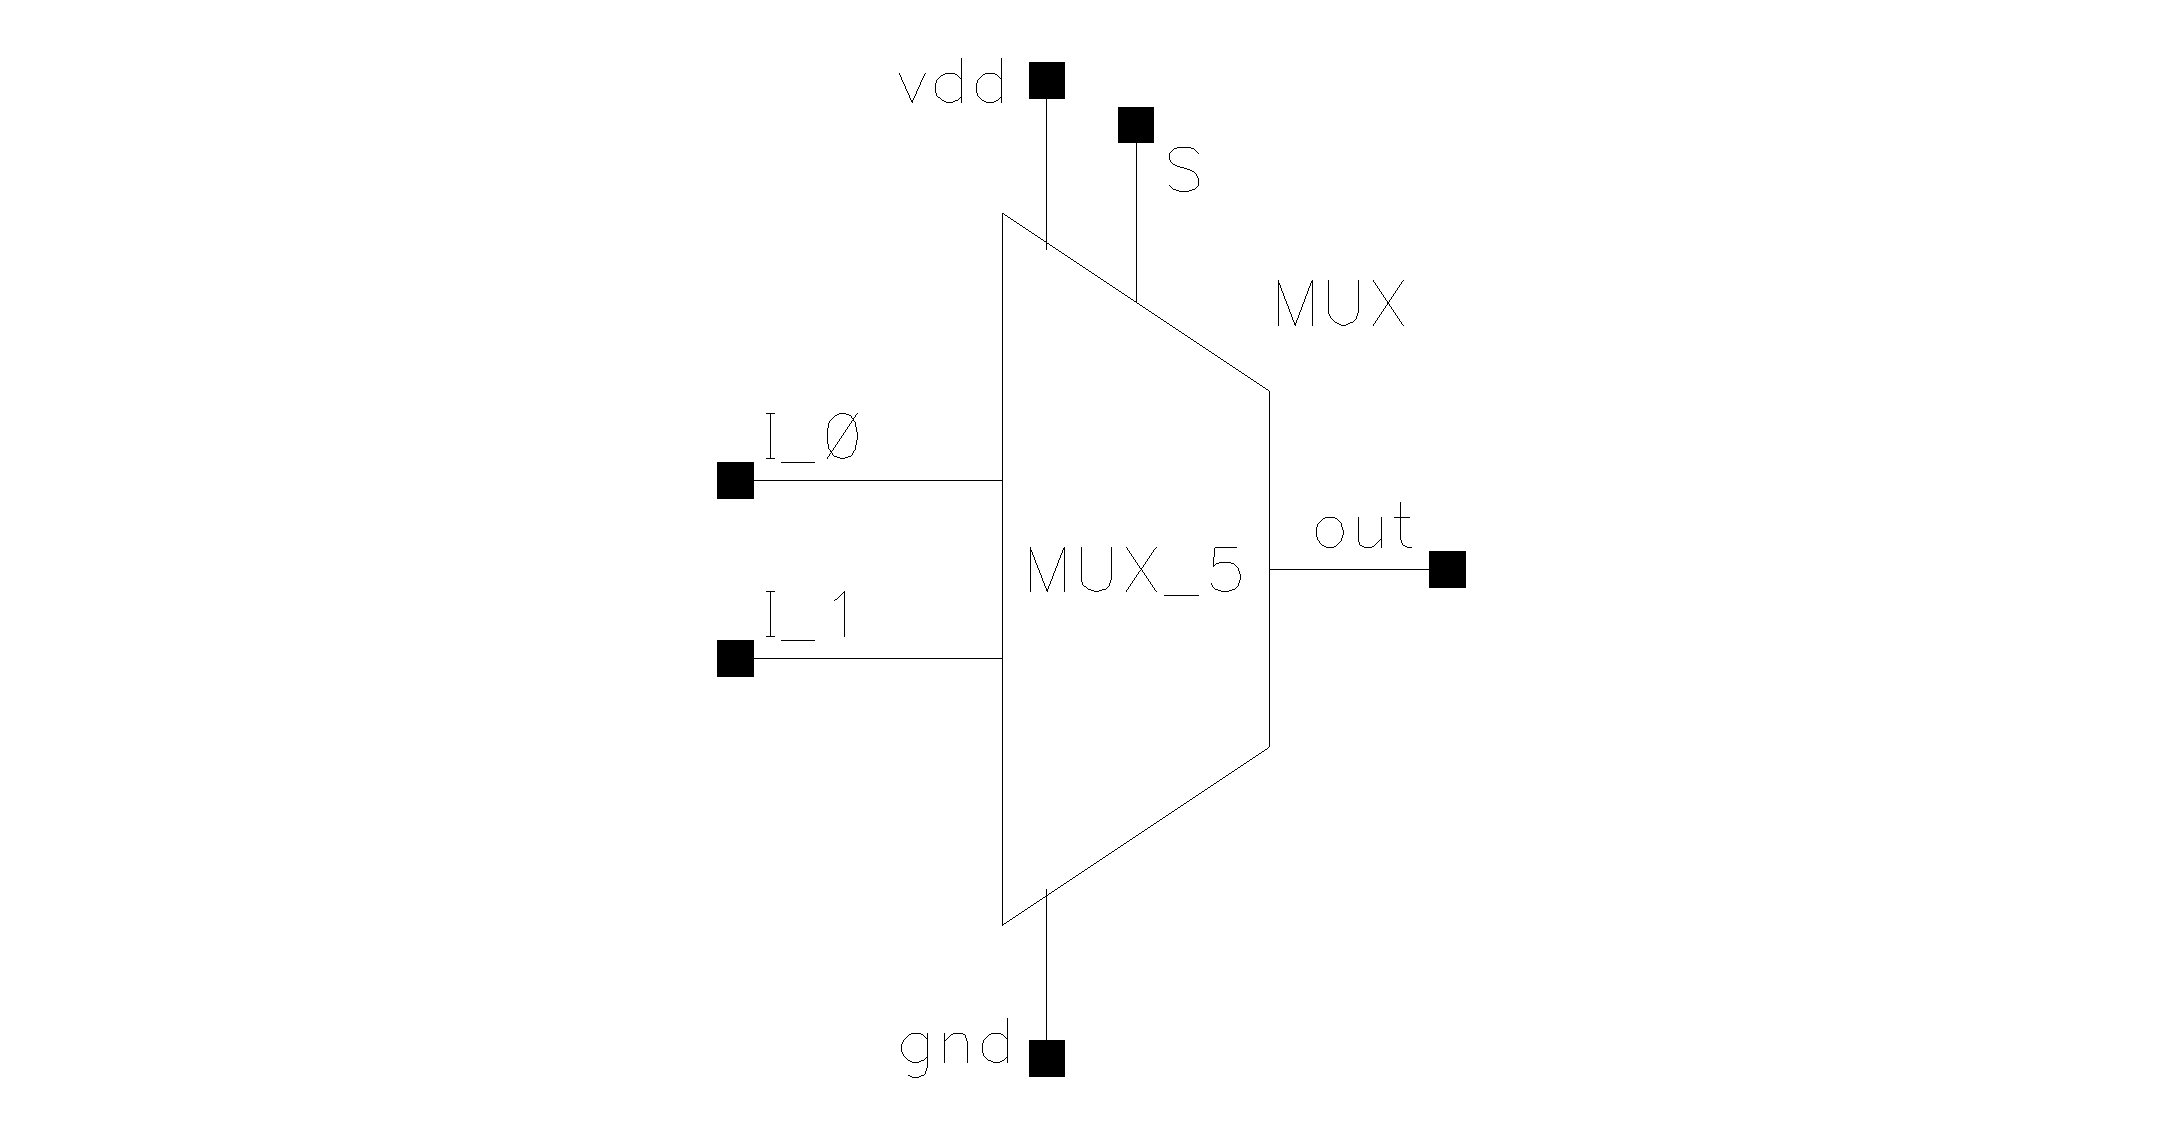
\includegraphics[width=\textwidth]{writeup/figures/mux_w2_opt_sym.png}
        \caption{}
        \label{fig:mux_w2_opt_sym}
    \end{subfigure}
    \caption{Optimized MUX for third stage: schematic and its corresponding symbol}
    \label{fig:mux2_opt_comparison}
\end{figure}

\begin{figure}[H]
    \centering
    % Subfigure A
    \begin{subfigure}[b]{0.48\textwidth}
        \centering
        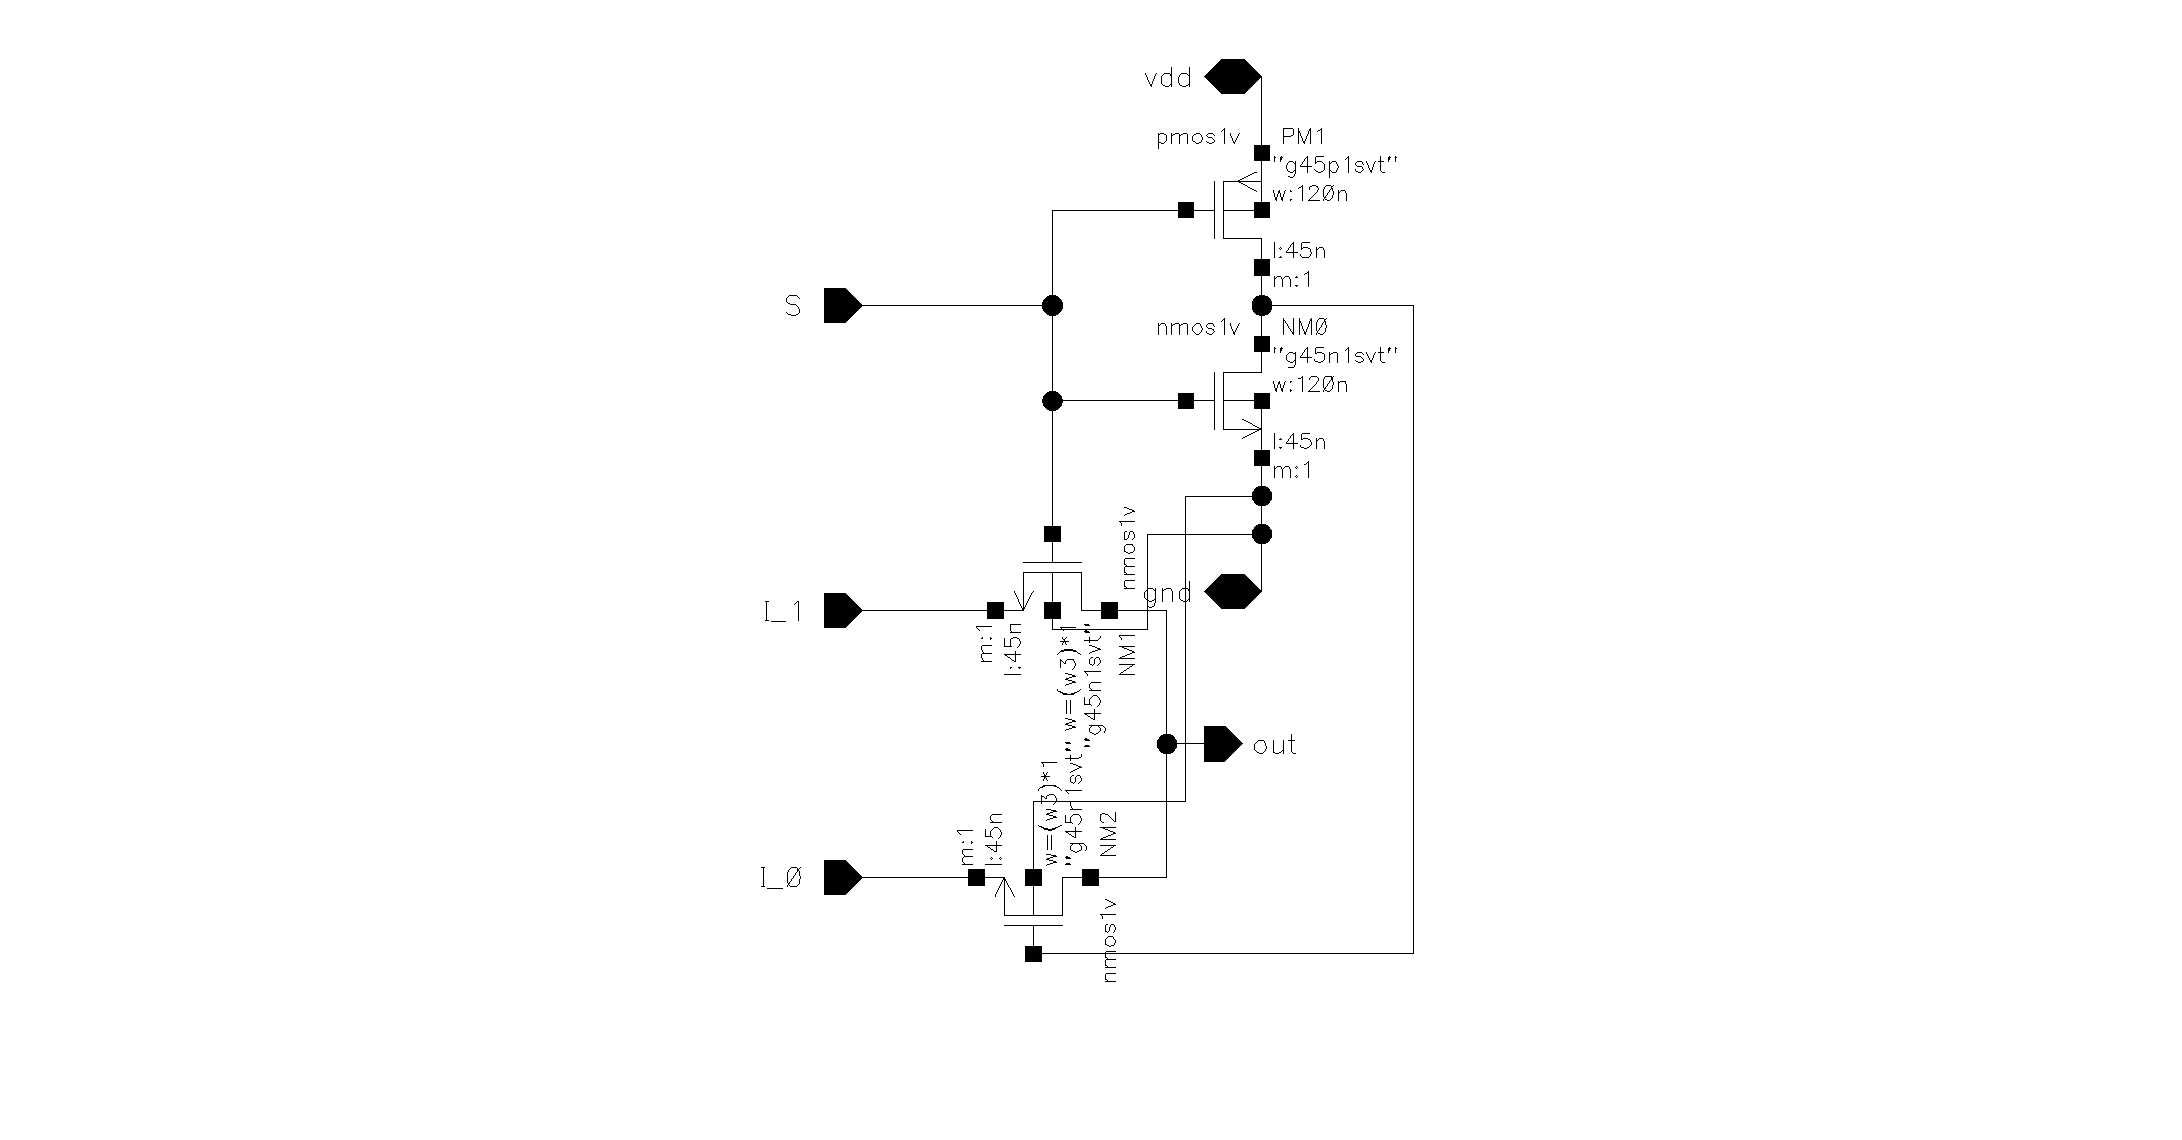
\includegraphics[width=\textwidth]{writeup/figures/mux_w3_opt.png}
        \caption{}
        \label{fig:mux_w3_opt}
    \end{subfigure}
    \hfill
    % Subfigure B
    \begin{subfigure}[b]{0.48\textwidth}
        \centering
        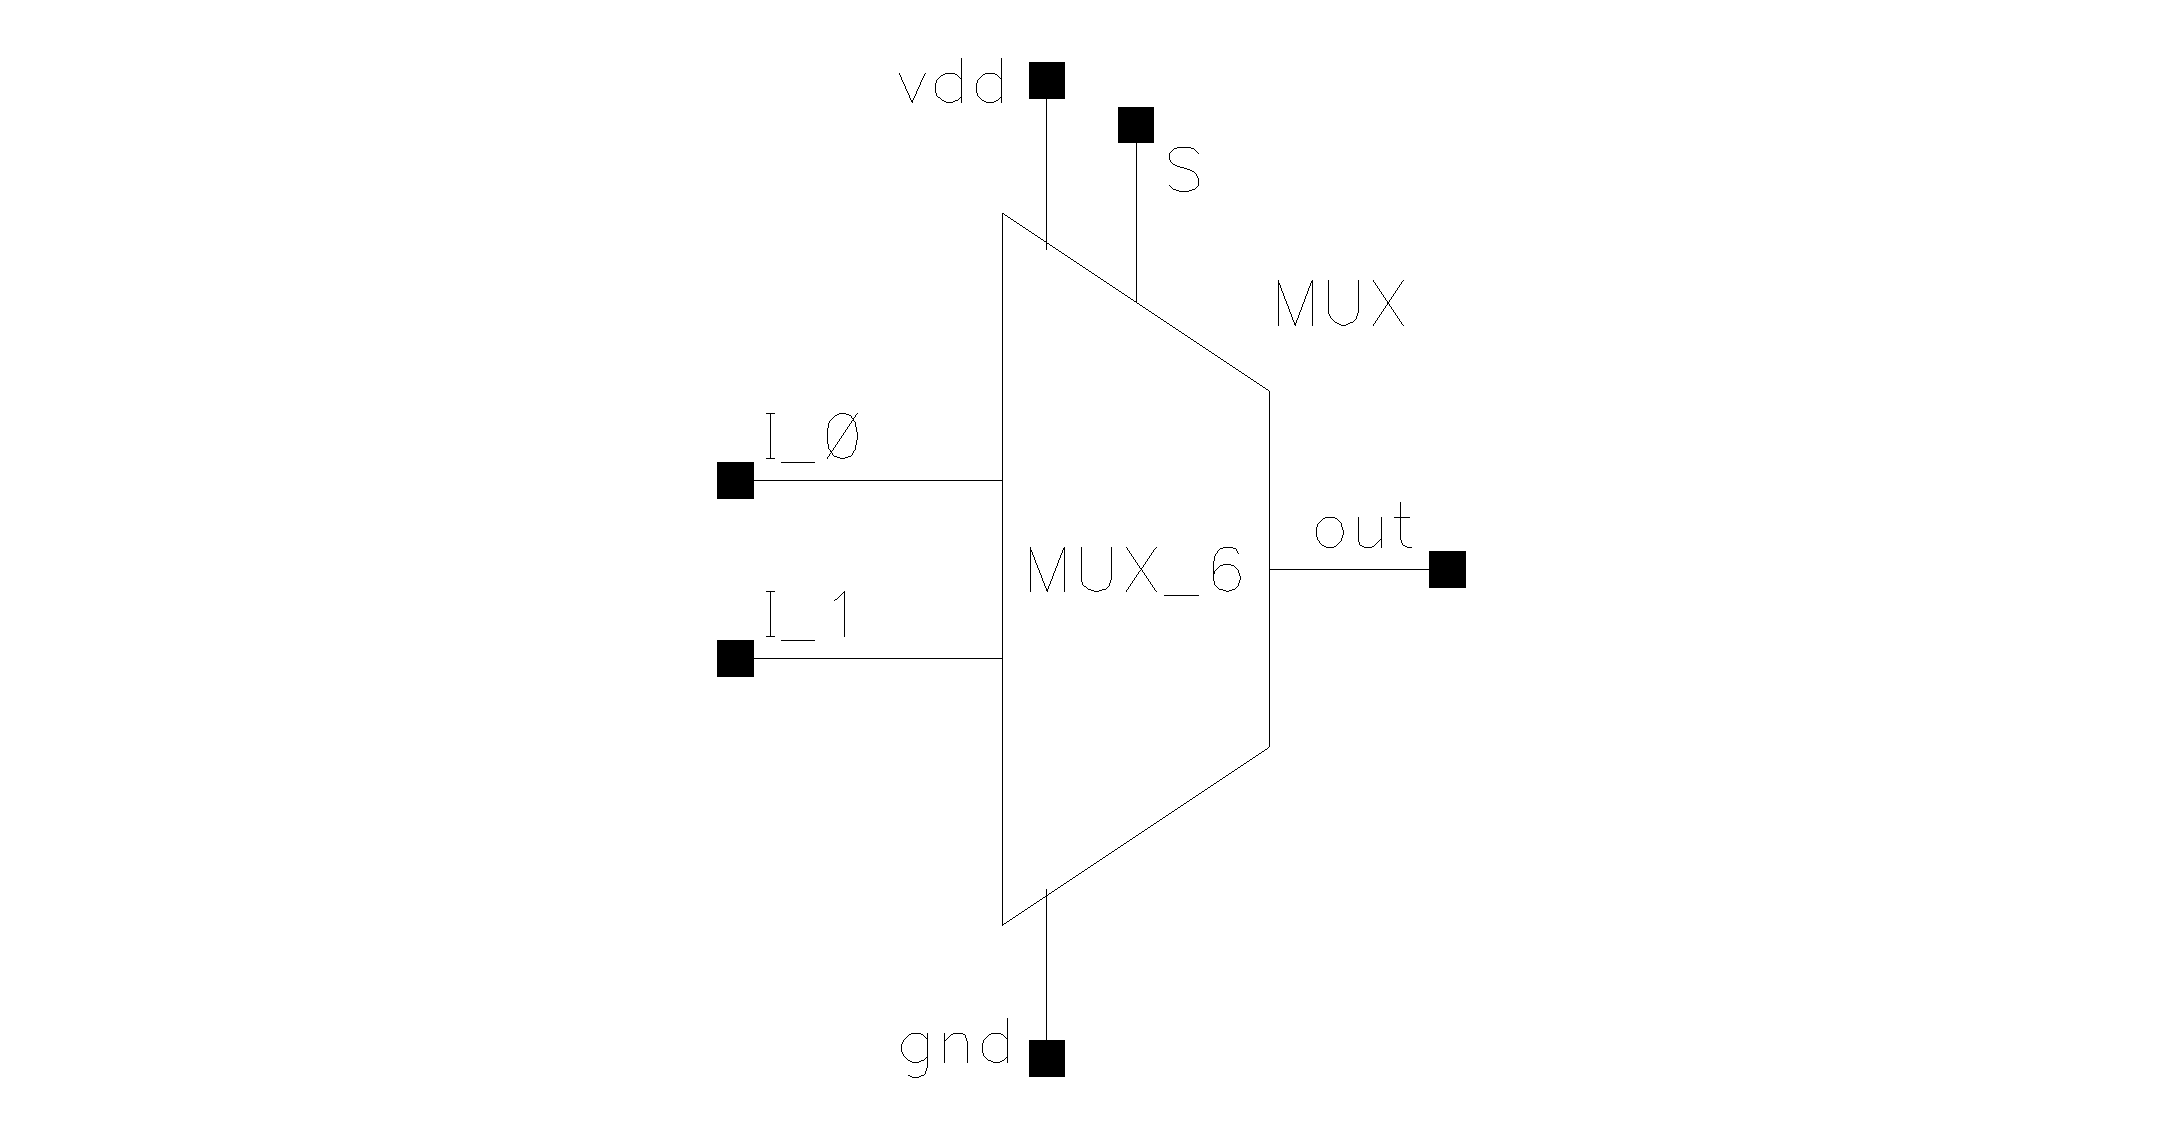
\includegraphics[width=\textwidth]{writeup/figures/mux_w3_opt_sym.png}
        \caption{}
        \label{fig:mux_w3_opt_sym}
    \end{subfigure}
    \caption{Optimized MUX for last stage: schematic and its corresponding symbol}
    \label{fig:mux3_opt_comparison}
\end{figure}

\begin{figure}[H]
    \centering
    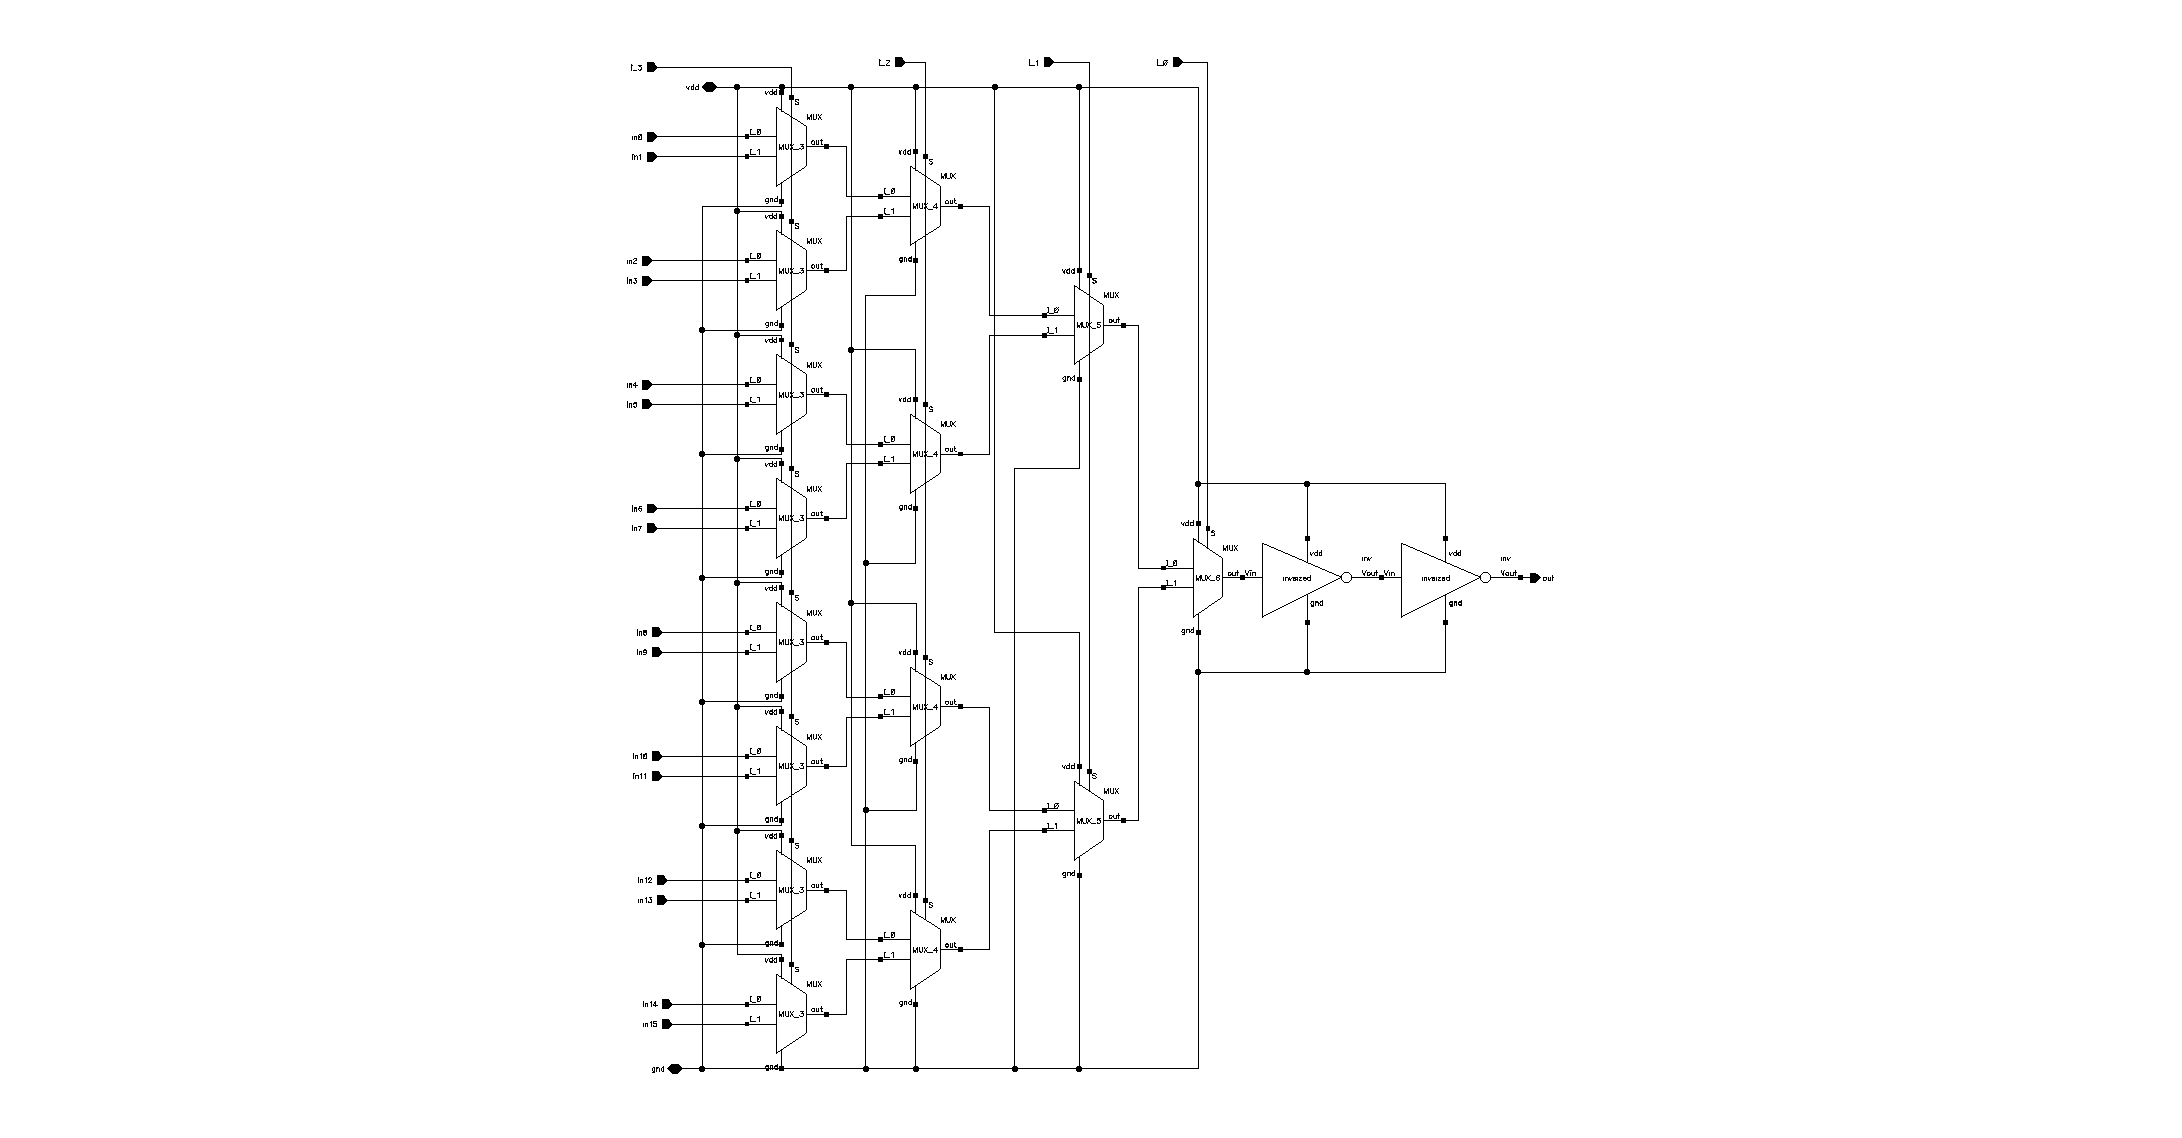
\includegraphics[width=0.8\linewidth]{writeup//figures/updated_delay_opt_LUTschem.png}
    \caption{}
\end{figure}

\begin{figure}[H]
    \centering
    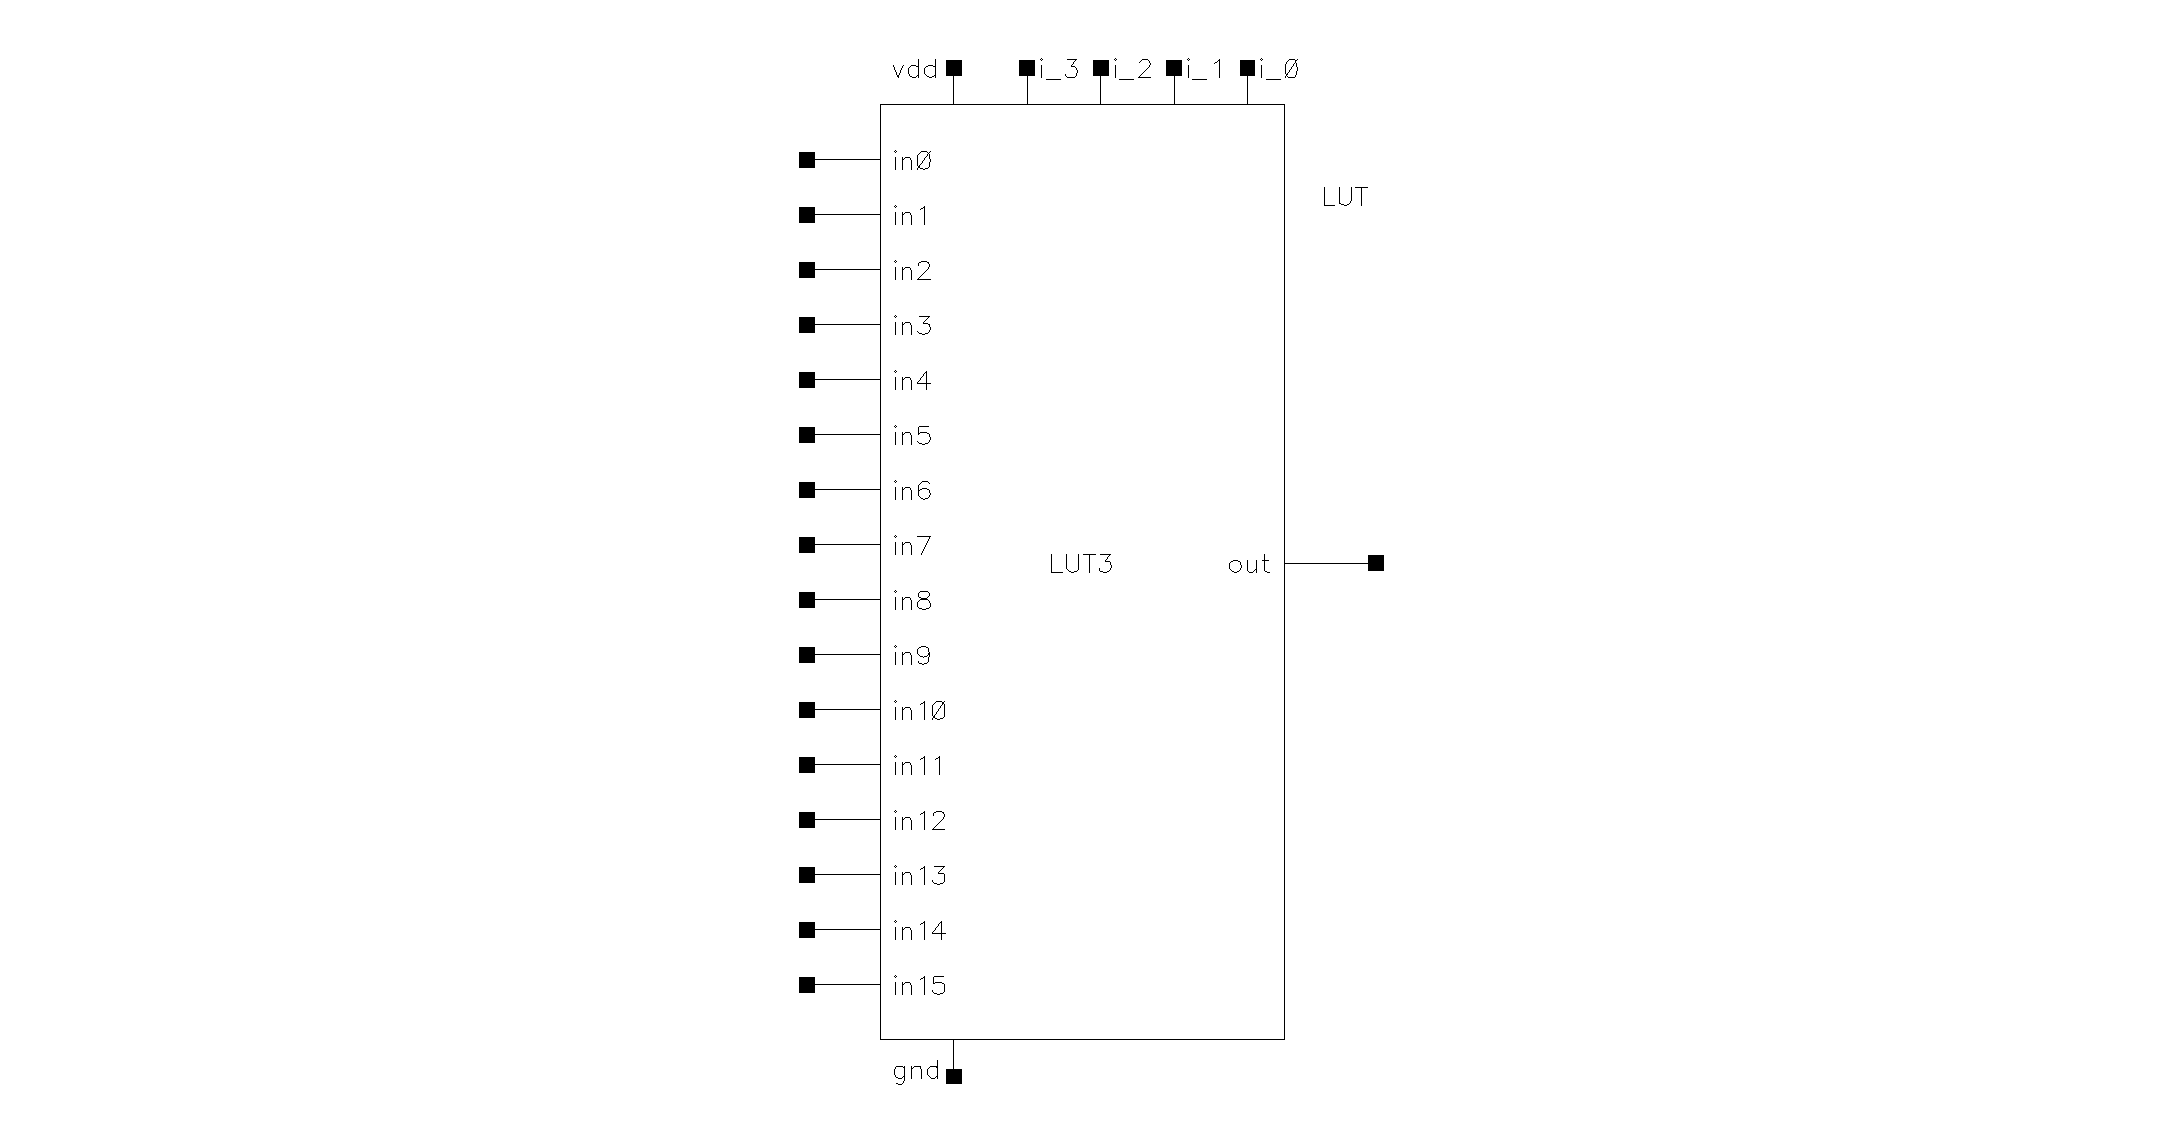
\includegraphics[width=0.8\linewidth]{writeup//figures/updated_delay_opt_LUTsym.png}
    \caption{}
\end{figure}

\newpage

\subsection{Optimization Process}

To minimize the propagation delay of the 16:1 LUT, a systematic multi-stage optimization approach was employed. The transistor widths in the 2:1 MUX structures were parameterized as $w_{\text{mux}}$, and those in the output restoring buffer were parameterized as $w_{\text{buf}}$. The optimization began by performing a parametric sweep of $w_{\text{mux}}$ while holding $w_{\text{buf}}$ constant at its minimum size. For each sweep, the delay was extracted as the time difference between the $0.6~\text{V}$ crossing points of the input and output waveforms, and the optimal $w_{\text{mux}}$ was identified as the width corresponding to the minimum of the delay curve.  

After obtaining the optimal $w_{\text{mux}}$, a similar sweep was conducted for $w_{\text{buf}}$, this time keeping $w_{\text{mux}}$ fixed at its previously determined value. This alternating optimization process was iteratively repeated—first sweeping $w_{\text{mux}}$ while fixing $w_{\text{buf}}$, then sweeping $w_{\text{buf}}$ while fixing $w_{\text{mux}}$—until both parameters converged to stable values. The iterative analysis converged to an optimal configuration of $w_{\text{mux}} = 208~\text{nm}$ and $w_{\text{buf}} = 120~\text{nm}$, corresponding to the minimum feature size allowed in the process.  

Following the global optimization, a more granular, stage-dependent optimization was explored to further reduce overall delay. Since the 16:1 LUT is composed of multiple hierarchical stages of 2:1 MUXes, each stage experiences progressively lighter capacitive loading toward the final output. Therefore, using the same transistor sizing for all stages is suboptimal—early stages drive larger effective capacitances and thus benefit from wider devices, while later stages can remain narrower without impacting speed. To exploit this behavior, different $w_{\text{mux}}$ values were assigned to each stage, and a comprehensive parametric sweep was performed across all valid combinations to identify the configuration yielding the shortest propagation delay.  

In this refined analysis, the buffer width was fixed at the previously optimized $w_{\text{buf}} = 120~\text{nm}$. The resulting optimized transistor widths were applied to each stage of the LUT’s MUX network, producing a fully optimized design that balances drive strength and parasitic loading across the hierarchy.  

The figures that follow illustrate the parametric sweeps and delay trends that guided the selection of these optimal transistor dimensions.

\subsubsection*{Optimization of 2 Variables: $w_{\text{buf}}$ \& $w_{\text{mux}}$}

\begin{figure}[H]
    \centering
    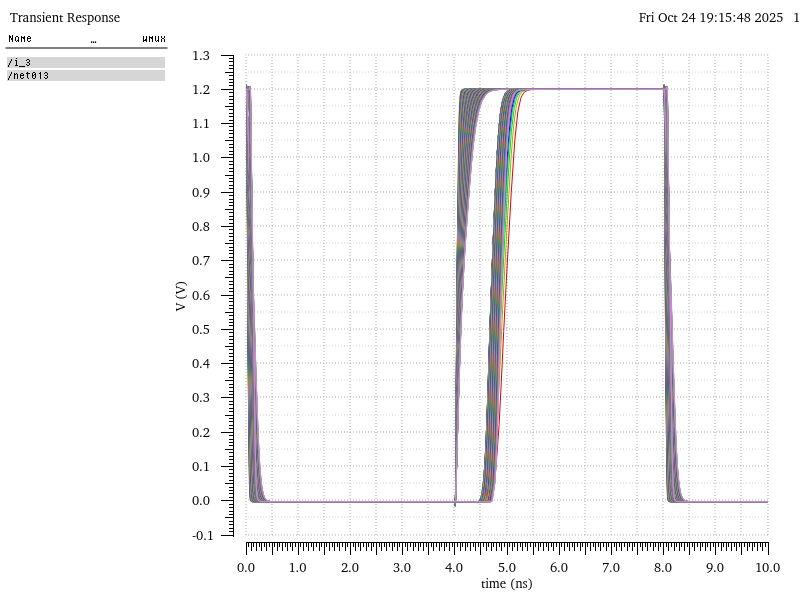
\includegraphics[width=0.5\linewidth]{writeup//figures/wmux_parametric_sweep2.png}
    \caption{1st parametric sweep of wmux with wbuf held constant}
\end{figure}

\begin{figure}[H]
    \centering
    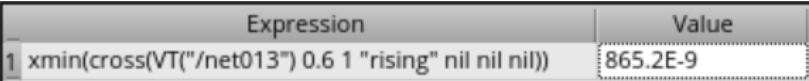
\includegraphics[width=0.5\linewidth]{writeup//figures/wmux2.png}
    \caption{Value obtained from 1st parametric sweep of wmux with wbuf held constant}
\end{figure}

\begin{figure}[H]
    \centering
    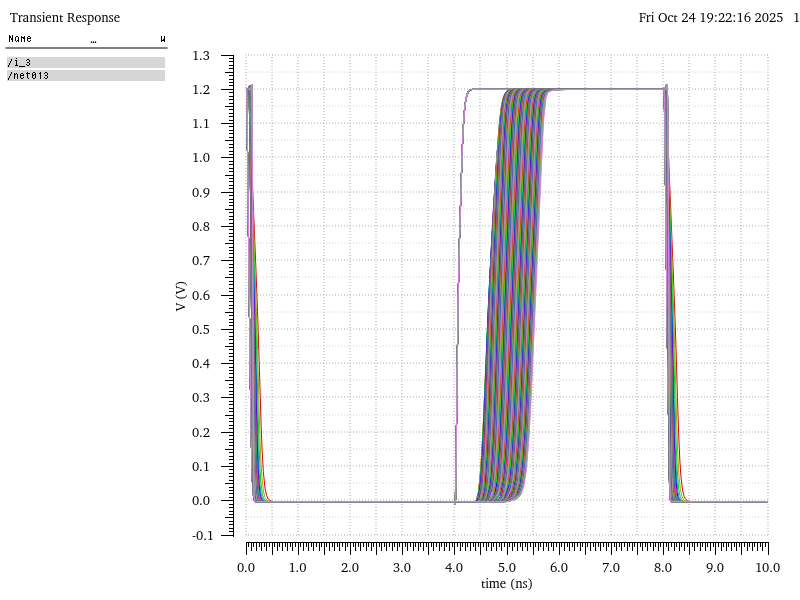
\includegraphics[width=0.5\linewidth]{writeup//figures/wbuf_parametric_sweep2.png}
    \caption{1st parametric sweep of wbuf with wmux held constant at value found in previous sweep}
\end{figure}

\begin{figure}[H]
    \centering
    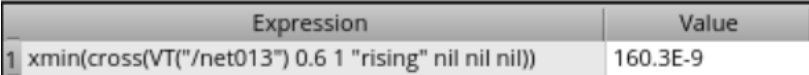
\includegraphics[width=0.5\linewidth]{writeup//figures/wbuf2.png}
    \caption{Value obtained from 1st parametric sweep of wbuf with wmux held constant at value found in previous sweep}
\end{figure}

\begin{figure}[H]
    \centering
    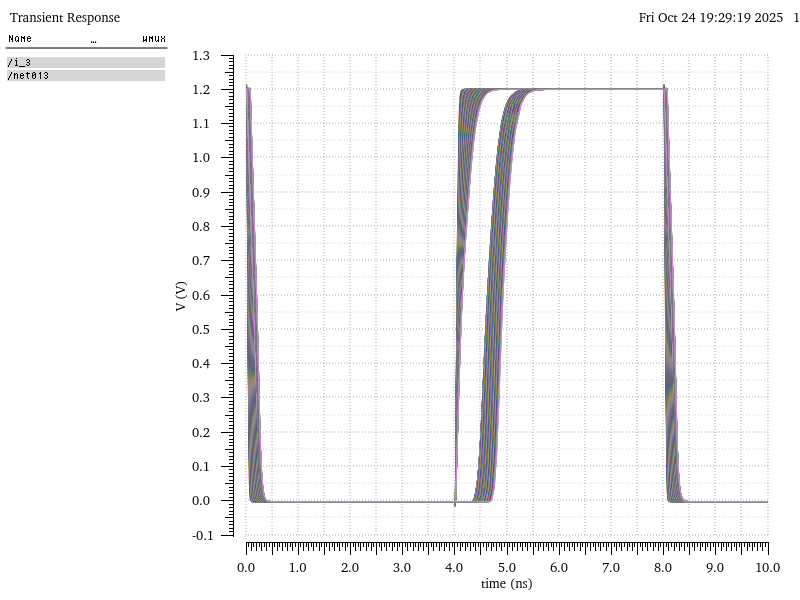
\includegraphics[width=0.5\linewidth]{writeup//figures/wmux_parametric_sweep3.png}
    \caption{2nd parametric sweep of wmux with wbuf held constant}
\end{figure}

\begin{figure}[H]
    \centering
    
\includegraphics[width=0.5\linewidth]{writeup//figures/wmux3.png}
    \caption{Value obtained from 2nd parametric sweep of wmux with wbuf held constant}
\end{figure}

\begin{figure}[H]
    \centering
    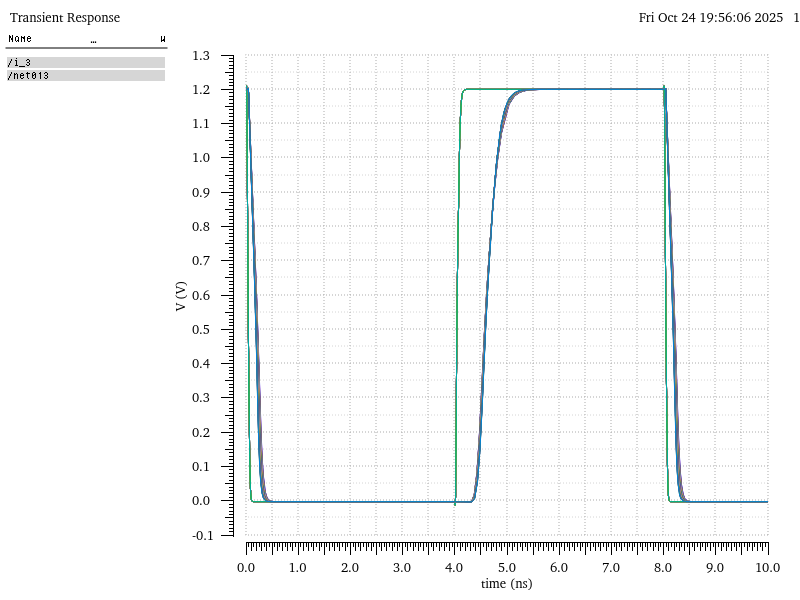
\includegraphics[width=0.5\linewidth]{writeup//figures/wbuf_parametric_sweep3.png}
    \caption{2nd parametric sweep of wbuf with wmux held constant at value found in previous sweep}
\end{figure}

\begin{figure}[H]
    \centering
    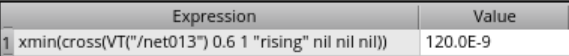
\includegraphics[width=0.5\linewidth]{writeup//figures/wbuf3.png}
    \caption{Value obtained from 2nd parametric sweep of wbuf with wmux held constant at value found in previous sweep}
\end{figure}

\begin{figure}[H]
    \centering
    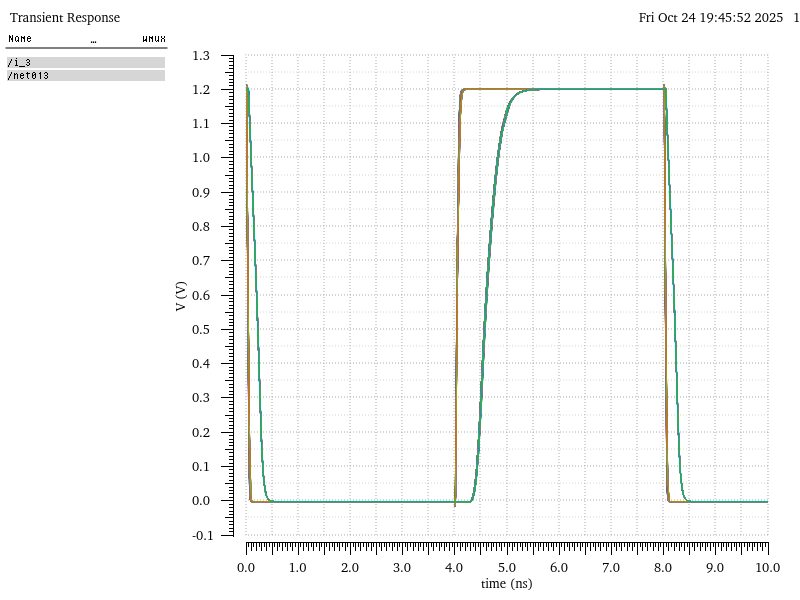
\includegraphics[width=0.5\linewidth]{writeup//figures/wmux_parametric_sweep4.png}
    \caption{3rd parametric sweep of wmux with wbuf held constant}
\end{figure}

\begin{figure}[H]
    \centering
    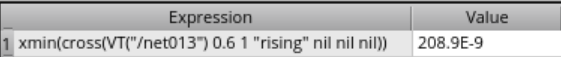
\includegraphics[width=0.5\linewidth]{writeup//figures/wmux4.png}
    \caption{Value obtained from 3rd parametric sweep of wmux with wbuf held constant}
\end{figure}

\begin{figure}[H]
    \centering
    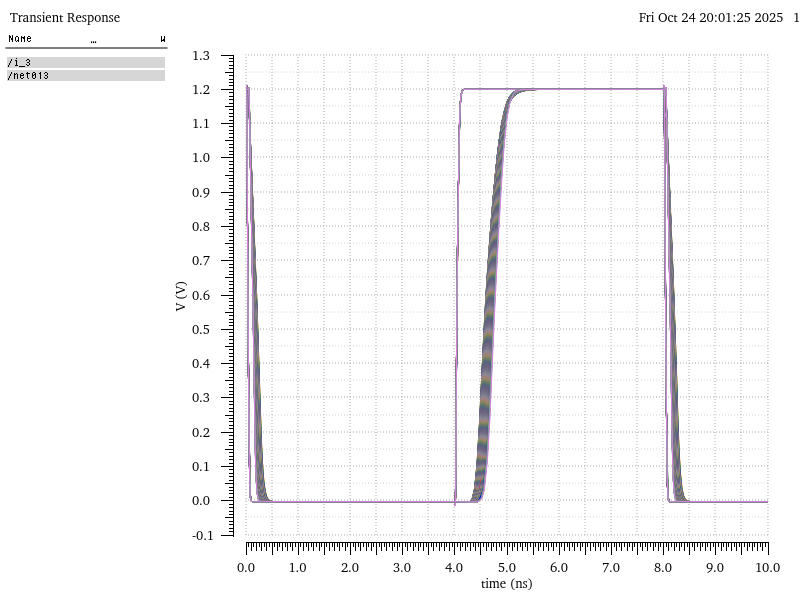
\includegraphics[width=0.5\linewidth]{writeup//figures/wbuf_parametric_sweep4.png}
    \caption{3rd parametric sweep of wbuf with wmux held constant at value found in previous sweep}
\end{figure}

\begin{figure}[H]
    \centering
    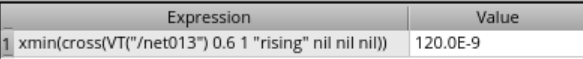
\includegraphics[width=0.5\linewidth]{writeup//figures/wbuf4.png}
    \caption{Value obtained from 3rd parametric sweep of wbuf with wmux held constant at value found in previous sweep}
\end{figure}

\subsubsection*{Optimization of 4 Variables: $w_0$, $w_1$, $w_2$ \& $w_3$}

\begin{figure}[H]
    \centering
    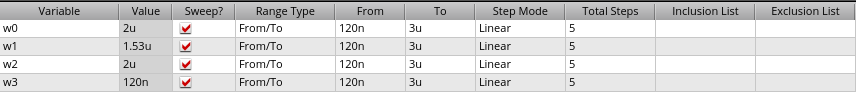
\includegraphics[width=0.5\linewidth]{writeup//figures/wmux_all_parametric_sweep_setup.png}
    \caption{Setup for parametric analysis of all combinations for individual widths of the pass transistors across all 4 stages of the MUXs}
\end{figure}

\begin{figure}[H]
    \centering
    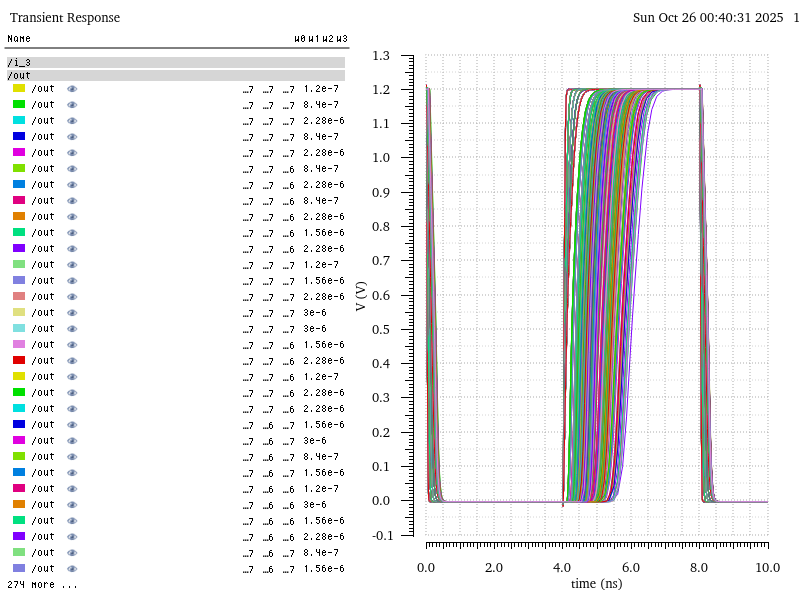
\includegraphics[width=0.5\linewidth]{writeup//figures/wmux_all_parametric_sweep.png}
    \caption{Transient response of the parametric analysis for all combinations for individual widths of the pass transistors across all 4 stages of the MUXs}
\end{figure}

\begin{figure}[H]
    \centering
    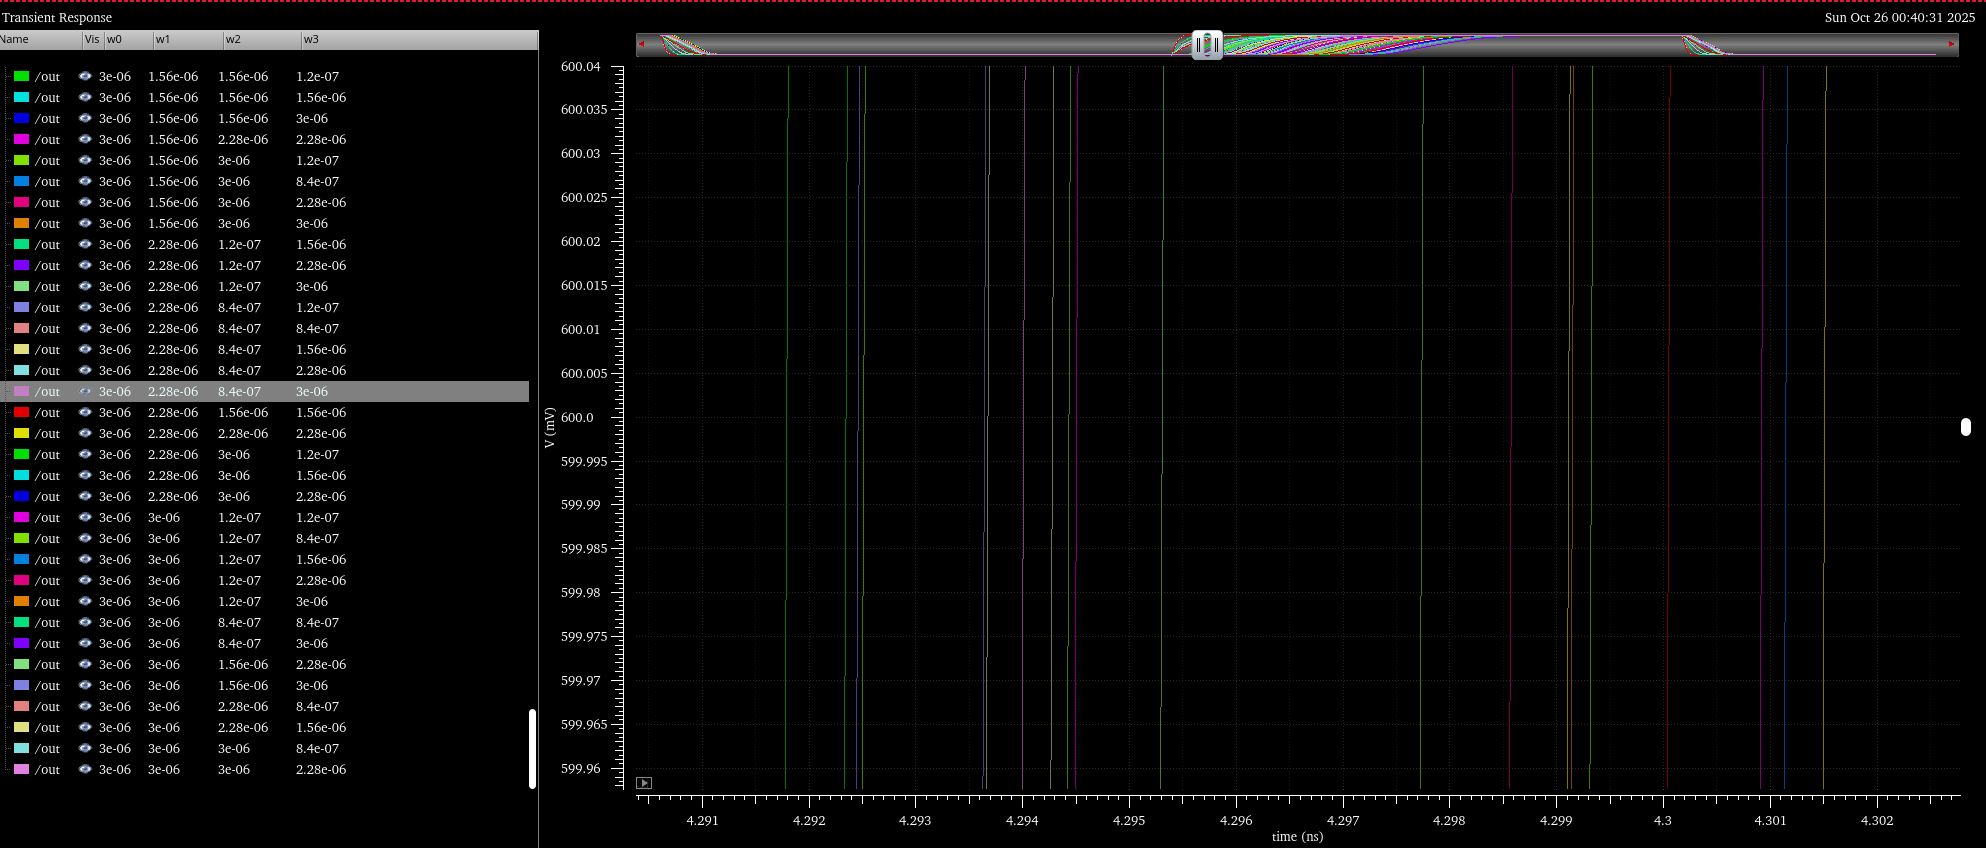
\includegraphics[width=\linewidth]{writeup//figures/wmux_all_zoomed_parametrics_weep2.png}
    \caption{Setup for parametric analysis of all combinations for individual widths of the pass transistors across the 4 stages of the MUXs. $w_1$ found as \textbf{2.28u}}
\end{figure}

\begin{figure}[H]
    \centering
    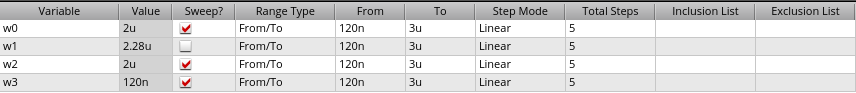
\includegraphics[width=0.5\linewidth]{writeup//figures/wmux_3_parametric_sweep_setup.png}
    \caption{Setup for parametric analysis of all combinations for individual widths of the pass transistors across all 4 stages of the MUXs}
\end{figure}

\begin{figure}[H]
    \centering
    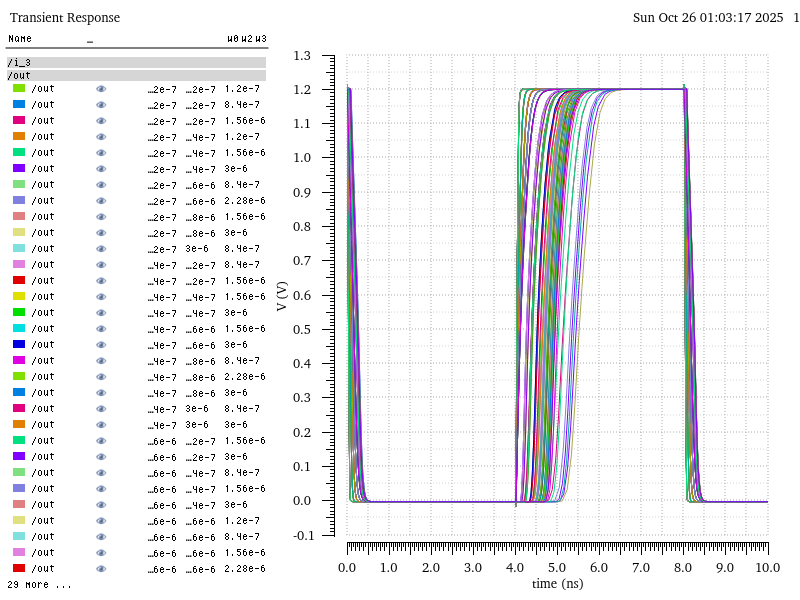
\includegraphics[width=0.5\linewidth]{writeup//figures/wmux_3_parametric_sweep.png}
    \caption{Transient response of the parametric analysis for all combinations for individual widths of the pass transistors across all 4 stages of the MUXs}
\end{figure}

\begin{figure}[H]
    \centering
    \includegraphics[width=0.8\linewidth]{writeup//figures/wmux_3_parametrics_weep.png}
    \caption{Setup for parametric analysis of all combinations for individual widths of the pass transistors across the 4 stages of the MUXs. $w_0$ also found as \textbf{2.28u}}
\end{figure}

\begin{figure}[H]
    \centering
    \includegraphics[width=0.5\linewidth]{writeup//figures/wmux_2_parametric_sweep_setup.png}
    \caption{Setup for parametric analysis of all combinations for individual widths of the pass transistors across all 4 stages of the MUXs}
\end{figure}

\begin{figure}[H]
    \centering
    \includegraphics[width=0.5\linewidth]{writeup//figures/wmux_2_parametric_sweep.png}
    \caption{Transient response of the parametric analysis for all combinations for individual widths of the pass transistors across all 4 stages of the MUXs}
\end{figure}

\begin{figure}[H]
    \centering
    \includegraphics[width=\linewidth]{writeup//figures/wmux_2_parametrics_weep.png}
    \caption{Setup for parametric analysis of all combinations for individual widths of the pass transistors across the 4 stages of the MUXs. $w_3$ found as \textbf{840n}}
\end{figure}

\begin{figure}[H]
    \centering
    \includegraphics[width=0.5\linewidth]{writeup//figures/wmux_1_parametric_sweep_setup.png}
    \caption{Setup for parametric analysis of all combinations for individual widths of the pass transistors across all 4 stages of the MUXs}
\end{figure}

\begin{figure}[H]
    \centering
    \includegraphics[width=0.5\linewidth]{writeup//figures/wmux_1_parametric_sweep.png}
    \caption{Transient response of the parametric analysis for all combinations for individual widths of the pass transistors across all 4 stages of the MUXs}
\end{figure}

\begin{figure}[H]
    \centering
    \includegraphics[width=0.8\linewidth]{writeup//figures/wmux_1_parametrics_weep.png}
    \caption{Setup for parametric analysis of all combinations for individual widths of the pass transistors across the 4 stages of the MUXs. $w_1$ found as a value greater than the maximum value of 10u, so set at the upper limit of \textbf{10u}.}
\end{figure}

\newpage

\subsubsection*{Summary Table}

\begin{table}[H]
\centering

\begin{tabular}{|c|c|c|}
\hline
\textbf{Parameter} & \textbf{Description} & \textbf{Optimized Width} \\ \hline
$w_{\text{buf}}$ & Output buffer transistor width & 120~nm \\ \hline
$w_{0}$ & Pass transistor width for Stage~0 (closest to output) & 2.28~$\mu$m \\ \hline
$w_{1}$ & Pass transistor width for Stage~1 & 10.0~$\mu$m \\ \hline
$w_{2}$ & Pass transistor width for Stage~2 & 2.28~$\mu$m \\ \hline
$w_{3}$ & Pass transistor width for Stage~3 (input stage) & 840~nm \\ \hline
\end{tabular}
\label{tab:optimized_widths}
\caption{Summary of Optimized Transistor Widths for LUT Design}
\end{table}

\newpage

\subsubsection*{RC Model and Elmore Delay}

We also attemtped to analytically understand although our parametric analysis yielded much more significant improvements. Nonetheless, our calculations are shwon below.

\begin{figure}[H]
    \centering
    \includegraphics[width=\linewidth]{writeup//figures/elmore.jpeg}
    \caption{}
\end{figure}

\newpage

% ------------------ SECTION 7 ------------------
\section{Optimized Design Validation and Logical Test}
\subsection{Test Schematic and Case}
The muxes were designed the same way as the baseline design, but different variables were set for the widths of muxes in each stage. 

\begin{figure}[H]
    \centering
    \includegraphics[width=\linewidth]{writeup//figures/optimized_LUT_validation_testschem.png}
    \caption{Used the same schematic as baseline for validation, ubdating the LUT used to the one with optimized widths.}
\end{figure}



\newpage

\subsection{Simulation Results}
\subsubsection*{2:1 MUX Subcircuit Validation}
\begin{figure}[H]
    \centering
    \includegraphics[width=\linewidth]{writeup//figures/muxsubval.png}
    \caption{}
\end{figure}

The same subcircuit was used as the baseline. Widths were varied according to the stage, for optimization. In the subcircuit test, the select input \( S \) is toggled while \( I_0 \) and \( I_1 \) run as independent square waves. 
Whenever \( S \) is high, the output waveform overlays \( I_1 \) with only a small propagation delay; whenever \( S \) is low, the output overlays \( I_0 \). 
Each handoff can be observed at the transitions of \( S \): during every \( S=1 \) interval the output \( V_{\text{out}} \) matches \( I_1 \), and during every \( S=0 \) interval it matches \( I_0 \). 
This behavior corresponds to the expected logic equation 
\[
V_{\text{out}} = S \cdot I_1 + \overline{S} \cdot I_0
\]
for a 2:1 pass-gate multiplexer. 
The simulation therefore verifies that the subcircuit operates correctly.

\subsubsection*{16:1 LUT Validation}
\begin{figure}[H]
    \centering
    \includegraphics[width=\linewidth]{writeup//figures/lut_opt_validation_sim_updated.png}
    \caption{}
\end{figure}
The overall test schematic was the same for optimized compared to baseline, except the widths changed for each stage, based on a parametric sweep. After inputting the widths found from the sweep (see optimized delay measurement section), the following validation results were obtained.  For the full 16:1 LUT, all sixteen input combinations (\(2^4\)) were simulated by varying the four address lines from \(0000\) through \(1111\). 
In each address state, the output \(V_{\text{out}}\) aligns with exactly one corresponding data input. 
Specifically, when the address equals \(0000\), \(\text{IN}_0\) propagates to the output; as the address increments, \(\text{IN}_1, \text{IN}_2, \ldots, \text{IN}_{15}\) sequentially drive the output. 
Rising and falling edges on \(V_{\text{out}}\) coincide precisely with the selected input, while nonselected inputs show no coupling. 
Because all address combinations were verified and the output correctly reflected the selected data input each time, the 16:1 LUT simulation confirms correct functionality.

\newpage
% ------------------ SECTION 8 ------------------
\section{Optimized Delay Measurement}
\subsubsection{Test Schematic}
\begin{figure}[H]
    \centering
    \includegraphics[width=\linewidth]{writeup//figures/updated_delay_opt_testschem.png}
    \caption{}
\end{figure}

\newpage
\subsubsection*{Test Case}

To evaluate the worst-case propagation delay of the delay-optimized 16:1 LUT, the same input configuration and excitation scheme used in the baseline delay measurement were retained to ensure consistency in comparison. Data inputs \texttt{IN0} through \texttt{IN7} were tied to ground (0~V), while \texttt{IN8} through \texttt{IN15} were connected to $V_{DD}$. Separate ground and $V_{DD}$ connections were again provided for \texttt{IN0} and \texttt{IN15}, representing the boundary input conditions corresponding to the output transitions of interest.

The four address lines ($I_0, I_1, I_2, I_3$) were driven by \texttt{Vpulse} sources transitioning from low to high, generating the binary address sequence from 0000 to 1111. This ensured that the optimized LUT traversed every possible input state, activating the same critical switching path identified in the baseline test. Because $I_3$ served as the least significant bit (LSB), the signal path corresponding to $I_3$ still produced the longest propagation delay through the internal MUX hierarchy, allowing direct comparison with the baseline measurement. However, in this optimized configuration, the LUT instance was replaced with the version featuring stage-dependent transistor sizing, where each MUX stage was independently sized to balance drive strength and reduce overall path delay.

At the output node, the same capacitive loading condition was applied to replicate the baseline’s high fan-out scenario. Three NMOS transistors with widths of 10~µm, 10~µm, and 4~µm were connected in parallel to achieve an equivalent capacitive loading of approximately 200$C_G$, corresponding to a total effective width of 24~µm. This loading ensured realistic delay measurement under identical conditions, isolating the impact of the transistor width optimization within the LUT on the observed propagation delay.

\newpage

\subsection{Simulation Results and Metric Value}

\begin{figure}[H]
    \centering
    \includegraphics[width=0.8\linewidth]{writeup//figures/optimized_delay_ADEL_setup.png}
    \caption{}
\end{figure}

\begin{figure}[H]
    \centering
    \includegraphics[width=\linewidth]{writeup//figures/updated_delay_opt.png}
    \caption{}
\end{figure}
From the transient response, the measured $50\%$ crossing times are
\[
t_{\text{in},50\%\downarrow} = 4.119~\text{ns}, \quad
t_{\text{out},50\%\uparrow} = 4.272~\text{ns}, \quad
t_{\text{in},50\%\uparrow} = 8.115~\text{ns}, \quad
t_{\text{out},50\%\downarrow} = 8.196~\text{ns}.
\]
The propagation delays are therefore
\[
t_{PLH} = t_{\text{out},50\%\uparrow} - t_{\text{in},50\%\downarrow}
        = 4.272~\text{ns} - 4.119~\text{ns}
        = \boxed{0.153~\text{ns}},
\]
\[
t_{PHL} = t_{\text{out},50\%\downarrow} - t_{\text{in},50\%\uparrow}
        = 8.196~\text{ns} - 8.115~\text{ns}
        = \boxed{0.081~\text{ns}}.
\]
The average propagation delay is
\[
t_P = \frac{t_{PLH} + t_{PHL}}{2}
     = \frac{0.153 + 0.081}{2}
     = \boxed{0.117~\text{ns}}.
\]
The percentage deviation of each transition from the average is
\[
\frac{t_{PLH} - t_P}{t_P} \times 100 = \boxed{+30.8\%}, 
\qquad
\frac{t_{PHL} - t_P}{t_P} \times 100 = \boxed{-30.8\%}.
\]
Comparing against the baseline LUT delay of $t_{P,\text{baseline}} = 0.8275~\text{ns}$, the delay-optimized LUT exhibits a significant improvement:
\[
\text{Speedup} 
= \frac{t_{P,\text{baseline}} - t_P}{t_{P,\text{baseline}}} \times 100
= \frac{0.8275 - 0.117}{0.8275} \times 100
= \boxed{85.9\%~\text{faster}}.
\]

The worst-case delay is the longer of the two:
\[
t_{pd,worst} = \max(t_{PLH}, t_{PHL}) = 0.153\,\text{ns}
\]

Hence, the optimized LUT demonstrates nearly an order of magnitude reduction in propagation delay, indicating a substantial timing enhancement while maintaining consistent rise–fall symmetry.





\newpage

% ------------------ SECTION 9 ------------------
\section{Optimized Frequency Measurement}
\subsection{Test Schematic}
\begin{figure}[H]
    \centering
    \includegraphics[width=\linewidth]{writeup//figures/updated_delay_opt_testschem.png}
    \caption{}
\end{figure}
The test configuration used for the delay-optimized LUT follows the same structure as the schematic employed in the delay measurement setup, with the only modification being the introduction of a variable input frequency parameter $f$ for the frequency sweep. The first eight data inputs of the 16:1 LUT (\texttt{data<7:0>}) are tied to ground, while the remaining eight inputs (\texttt{data<15:8>}) are tied to $V_{DD}$, replicating the same logical data pattern used in the baseline analysis to maintain consistency across measurement conditions.

In this configuration, the LUT under test was replaced with the optimized version featuring non-uniform transistor sizing across the 2:1 MUX hierarchy. Each stage in the MUX tree was sized independently according to its position, with larger transistors assigned to deeper levels to minimize propagation delay and maintain balanced drive strength. The address inputs (\texttt{addr<3:0>}) were driven by pulse sources through a minimum-sized inverter chain to model realistic input loading conditions, while the input frequency was swept parametrically over a wide range of values. This setup enabled accurate extraction of the frequency limit at which the delay-optimized LUT continues to produce valid logic levels before signal degradation or timing violations occur due to insufficient propagation through the resized MUX network.

\newpage

\subsection{Simulation Results and Metric Value}

\begin{figure}[H]
    \centering
    \includegraphics[width=\linewidth]{writeup//figures/frequency_response_param_20_40_optimized.png}
    \caption{Frequency response at output of the buffer stage for optimized design}
\end{figure}
The steady-state response of the optimized LUT under a parametric input-frequency sweep is shown. After a short transient period, both the input and output exhibit periodic behavior, enabling accurate assessment of the post-optimization frequency performance. Each colored trace corresponds to a distinct excitation frequency in the sweep, and the preservation of clean, full-swing transitions across a broader frequency range demonstrates the success of the delay optimization.


\begin{figure}[H]
    \centering
    \includegraphics[width=\linewidth]{writeup//figures/max_frequencies_optimized.png}
    \caption{Extracting frequency value that allows for 85\% of VDD after buffer stage}
\end{figure}
From the steady-state frequency response of the optimized LUT, the peak output voltage at the buffer stage was recorded for each simulated input frequency. These maximum voltage values were then plotted as shown in in the figure, to determine the point at which the output amplitude drops below the acceptable logic-high threshold. As with the baseline analysis, the cutoff criterion was defined as 85\% of $V_{DD}$ (i.e., 1.02~V for $V_{DD}=1.2$~V), corresponding to the minimum voltage level required to ensure valid logic-high operation.

Based on this criterion, the maximum operating frequency of the delay-optimized LUT was extracted to be approximately \textbf{914~MHz}. Beyond this frequency, the output amplitude begins to degrade rapidly due to limited charge and discharge time within the MUX hierarchy and output buffer. Compared to the baseline cutoff frequency of 577~MHz, this represents an improvement of roughly \textbf{1.6$\times$}, confirming that the optimized sizing and hierarchical balancing successfully reduced propagation delay and extended the LUT’s high-frequency operational limit.


\newpage

% ------------------ SECTION 10 ------------------
\section{Optimized Energy Measurement}
\subsection{Test Schematic}

\begin{figure}[H]
    \centering
    \includegraphics[width=\linewidth]{writeup//figures/updated_energy_opt_testchem.png}
    \caption{}
\end{figure}

Individual \texttt{Vpulse} sources were again used to drive the address-line inverters in order to provide consistent input excitation across all test cases. The same measurement configuration as in the baseline setup was employed to ensure a direct comparison of active energy consumption. Specifically, the LUT and its output buffer were powered by separate supply sources, allowing for independent monitoring of the current drawn by the internal MUX hierarchy and the buffer stage.

In this optimized configuration, the LUT instance was replaced with the delay-optimized version featuring non-uniform transistor sizing across the 2:1 MUX stages. The transistor widths were strategically varied according to their stage position within the MUX hierarchy to minimize overall propagation delay while maintaining logical correctness. The instantaneous current through the LUT’s dedicated $V_{DD}$ source was recorded to capture the dynamic switching energy of the resized devices, while the output current was simultaneously measured to account for energy dissipated through the final buffer. The total energy consumption was then obtained by integrating these current waveforms over one complete address transition cycle, enabling direct comparison with the baseline LUT to assess the efficiency impact of the delay optimization.

\newpage

\subsection{Test Case}
The same address-cycling test case used for the baseline energy measurement was applied to the delay-optimized LUT to ensure a direct and fair comparison. The four address inputs i0–i3 were configured to toggle sequentially through all $2^4 = 16$ possible address states exactly once per simulation period, with \texttt{i3} serving as the least significant bit (LSB) and \texttt{i0} as the most significant bit (MSB). As before, the MSB was driven with a period of $16T$ and the LSB with a period of $2T$.

However, in this optimized configuration, the base period $T$ was updated to correspond to the new maximum operating frequency of the delay-optimized LUT determined from the frequency sweep, given by 
\[
T = \frac{1}{914{,}213{,}000}~\text{s}.
\]
This adjustment ensures that the timing relationship between address transitions matches the improved high-frequency capability of the optimized design. Using this updated period allows the LUT to cycle through all address combinations at its enhanced performance limit while maintaining identical logical transition behavior to the baseline test case.


\newpage

\subsection{Simulation Results and Metric Value}

\begin{figure}[H]
    \centering
    \includegraphics[width=0.8\linewidth]{writeup//figures/optimized_energy_currents.png}
    \caption{}
\end{figure}

\begin{figure}[H]
    \centering
    \includegraphics[width=\linewidth]{writeup//figures/optimized_energy_val.png}
    \caption{}
\end{figure}

The transient current waveforms in Fig. 63 show the instantaneous current drawn from the LUT’s dedicated $V_{DD}$ source (bottom) and the output node (top) as the optimized design cycles through all 16 possible address states at the maximum operating frequency. The $V_{DD}$ current waveform exhibits sharp periodic spikes corresponding to the dynamic charging of the internal pass-transistor network and the output buffer, while the output current waveform captures transient discharging events through the pass-transistor paths of the MUX hierarchy.

To determine the total active energy, both current waveforms were integrated over one complete address cycle and multiplied by $V_{DD} = 1.2~\text{V}$. The resulting total dynamic energy consumption for the optimized LUT design was found to be $\boxed{E_{\text{optimized}} = 332.2~\text{fJ}}$.

This energy value represents a significant reduction relative to the baseline design (\(E_{\text{baseline}} = 622.1~\text{fJ}\)), confirming that the sizing optimization effectively reduced parasitic charging and discharging losses. The improvement arises primarily from the hierarchical transistor width distribution, which minimizes capacitive loading in early MUX stages while preserving sufficient drive strength near the output buffer.

\newpage

% ------------------ SECTION 11 ------------------
\section{Comparison Table}

\begin{table}[H]
\centering
\begin{tabular}{|c|c|c|c|c|c|}
\hline
\textbf{Design} & \textbf{$t_{\text{PLH}}$ (ns)} & \textbf{$t_{\text{PHL}}$ (ns)} & \textbf{$t_{P}$ (ns)} & \textbf{Max Frequency (MHz)} & \textbf{Energy (fJ)} \\ \hline
Baseline & 0.58197 & 0.16704 & 0.3745 & 577.01 & 622.1  \\ \hline
Delay-Optimized & 0.153 & 0.081 & 0.117 & 914.213 & 332.2  \\ \hline
\end{tabular}
\label{tab:comparison}
\caption{Comparison of Baseline and Delay-Optimized 16:1 LUT Designs}
\end{table}

\noindent
The comparison summarized in Table 2 demonstrates the significant performance improvements achieved through the delay optimization of the LUT. The average propagation delay decreased from $t_P = 0.3745~\text{ns}$ in the baseline design to $0.117~\text{ns}$ in the optimized version, corresponding to a $68.8\%$ reduction and an effective speedup of approximately $3.2\times$. The worst-case delay, taken as the longer of the two transitions, decreased from $t_{PLH,\text{baseline}} = 0.58197~\text{ns}$ to $t_{PLH,\text{opt}} = 0.153~\text{ns}$, representing a $73.7\%$ improvement. This substantial reduction stems from stage-dependent transistor sizing within the hierarchical 2:1 MUX network, which mitigates cumulative RC delay and improves drive balance between successive stages.

Correspondingly, the maximum reliable operating frequency increased from $577.01~\text{MHz}$ to $914.213~\text{MHz}$, reflecting a $58.4\%$ enhancement in timing capability. In addition to the delay improvements, the total active energy per switching event decreased from $622.1~\text{fJ}$ to $332.2~\text{fJ}$, a $46.6\%$ reduction. Together, these results confirm that the optimized LUT achieves both higher speed and lower energy consumption. The largest proportional improvement occurs in the rising-edge path ($t_{PLH}$), verifying that the sizing optimization effectively targeted the dominant delay-limiting transition within the MUX hierarchy.



\end{document}